
\title{Report on the ITER Clite Shutdown Doserate Calculations}
\author{
  Andrew Davis \\
  Department of Engineering Physics\\
  College of Engineering \\
  The University of Wisconsin-Madison\\
  Madison, Wisconsin, 53706, \underline{USA}
  \and
  Mohamed Sawan \\
  Department of Engineering Physics\\
  College of Engineering \\
  The University of Wisconsin-Madison\\
  Madison, Wisconsin, 53706, \underline{USA}
  \and
  Paul P. H. Wilson \\
  Department of Engineering Physics\\
  College of Engineering \\
  The University of Wisconsin-Madison\\
  Madison, Wisconsin, 53706, \underline{USA}
  \and
  Elliott Biondo \\
  Department of Engineering Physics\\
  College of Engineering \\
  The University of Wisconsin-Madison\\
  Madison, Wisconsin, 53706, \underline{USA}
  \and
  Ahmed Ibrahim \\
  Radiation Transport Group\\
  Oak Ridge National Laboratory \\
  P.O. Box 2008 \\
  Oak Ridge, Tennessee 37831, \underline{USA}
  \and
  Patrick Shriwise \\
  Department of Engineering Physics\\
  College of Engineering \\
  The University of Wisconsin-Madison\\
  Madison, Wisconsin, 53706, \underline{USA}
}

\date{\today}

\documentclass[12pt]{article}
%\usepackage[printwatermark]{xwatermark}
%\usepackage{mathptmx}
%\usepackage{fouriernc}
\usepackage{times}
\usepackage{graphicx}
\usepackage{longtable}
\usepackage[acronym]{glossaries}
\usepackage[a4paper, portrait, margin=0.5in]{geometry}
\usepackage[table]{xcolor}
\usepackage[nottoc,numbib]{tocbibind}
\usepackage{subcaption}
\usepackage{multirow}
\usepackage{draftwatermark}
\SetWatermarkText{DRAFT}
\SetWatermarkScale{1}

%% define this page left blank
\newcommand*{\blankpage}{%
\vspace*{\fill}
\begin{center}
 \centering \textbf{This page intentionally left blank}
\end{center}
\vspace{\fill}}

%% to get lof in toc
\renewcommand{\listoffigures}{\begingroup
\tocsection
\tocfile{\listfigurename}{lof}
\endgroup}

%% to get lot in toc
\renewcommand{\listoftables}{\begingroup
\tocsection
\tocfile{\listtablename}{lot}
\endgroup}

%%\makenoidxglossaries
\makeglossaries
%% abreviations
\newacronym{aci}{ACI}{Advanced Computing Initiative}
\newacronym{advantg}{ADVANTG}{AutomateD VAriaNce reducTion Generator}
\newacronym{alara_c}{ALARA - [Code]}{Analytic and Laplacian Adaptive Radioactivity Analysis}
\newacronym{alara_p}{ALARA - [Principle]}{As Low As Reasonably Achievable}
\newacronym{cad}{CAD}{Computer Aided Design}
\newacronym{cadis}{CADIS}{Consistent Adjoint Driven Importance Sampling}
\newacronym{chtc}{CHTC}{Centre for High Throughput Computing}
\newacronym{d1s}{D1S}{ Direct One (1) Step}
\newacronym{dag}{DAG}{ Direct Accelerated Geometry}
\newacronym{dagmc}{DAGMC}{ Direct Accelerated Geometry Monte Carlo}
\newacronym{dd}{DD}{ Diagnostics Division}
\newacronym{endf}{ENDF}{Evaluated Nuclear Data File}
\newacronym{ep}{EP}{Equatorial Port}
\newacronym{epp}{EPP}{Equatorial Port Plug}
\newacronym{epi}{EPI}{Equatorial Port Interspace}
\newacronym{fendl}{FENDL}{Fusion Evaluated Nuclear Data Library}
\newacronym{fwcadis}{FW-CADIS}{Forward Weighted - Consistent Adjoint Driven Importance Sampling}
\newacronym{gepp}{GEPP}{Generic Equatorial Port Plug}
\newacronym{icrp}{ICRP}{International Commission on Radiation Protection}
\newacronym{io}{IO}{ITER Organisation}
\newacronym{lp}{LP}{Lower Port}
\newacronym{lpp}{LPP}{Lower Pumping Port}
\newacronym{mcnp}{MCNP}{Monte Carlo N Particle}
\newacronym{moab}{MOAB}{Mesh Oriented datABase}
\newacronym{ornl}{ORNL}{Oak Ridge National Laboratory}
\newacronym{pi}{PI}{Port Interspace}
\newacronym{pyne}{PyNE}{Python for Nuclear Engineering}
\newacronym{r2s}{R2S}{Rigorous Two [2] Step}
\newacronym{sdr}{SDR}{Shutdown Dose Rate}
\newacronym{ta}{TA}{Task Agreement}
\newacronym{up}{UP}{Upper Port}
\newacronym{upp}{UPP}{Upper Port Plug}
\newacronym{upi}{UPI}{Upper Port Interspace}
\newacronym{uw}{UW}{The University of Wisconsin}
\begin{document}
\maketitle
\newpage
\tableofcontents
\newpage
\listoffigures
\newpage
\listoftables
\newpage
\section*{Acronyms}
 \gls{aci} \\ 
 \gls{advantg} \\ \gls{alara_c} \\
 \gls{alara_p} \\ \gls{cad} \\
 \gls{cadis} \\  \gls{chtc} \\
 \gls{d1s} \\
 \gls{dag} \\
 \gls{dagmc} \\ \gls{dd} \\
 \gls{endf} \\ \gls{ep} \\
 \gls{epp} \\ \gls{epi} \\
 \gls{fendl} \\ \gls{fwcadis} \\
 \gls{gepp} \\ \gls{icrp} \\
 \gls{io} \\ \gls{lp} \\
 \gls{lpp} \\ \gls{mcnp} \\
 \gls{moab} \\ \gls{ornl} \\
 \gls{pi} \\ \gls{pyne} \\
 \gls{r2s} \\ \gls{sdr} \\
 \gls{ta} \\ \gls{up} \\
 \gls{upp} \\ \gls{upi}

% \printnoidxglossaries[type=\acronymtype]
%\printglossary
%\printglossary[type=\acronymtype]
% none of these work, but should

\newpage
\section*{Executive Summary}
The results contained within this report show the results of complex 3D neutron
\& photon transport simulations to determine the shutdown photon dose rate
resulting from the neutron activation of structural materials within a
representative model of the ITER device. There are several ongoing questions
regarding the correct level of \gls{sdr} photon dose in the equatorial and upper port
regions of ITER.
\\
\\
The neutron results showed....
\\
\\
The activation results showed ....
\\
\\
The photon results showed ....
\\
\\
This analysis focused on only shutdown photon sources, and therefore does not
contain prompt photon doses.
\newpage
\blankpage
\newpage
\section*{Abstract}
This report provides the methology, input data, assumptions and results for a
full analysis of neutron, neutron induced activation and the subsequent
transport of residual decay photons in a reference ITER \gls{cad} model. The purpose
of the analysis was to (1) establish a baseline result for the shutdown photon
doserate around the ITER device and (2) determine the effect upon the \gls{sdr} of a
thin B$_4$C layer added to the plasma-side of the bioshield. A differentiating
factor in this analysis relative to others is the level of detail present in
the ports. The \gls{up} contained a detailed diagnostic model along side detailed \gls{pi}
equipment upto the bioshield plug. Similarly, the \gls{ep} contained the \gls{dd} model of
an \gls{epp} with diagnostic drawers and significant quantities of internal B$_4$C
shielding, the \gls{ep} interspace contained detailed models of rails, racks and
support frames out to the bioshield. The \gls{lpp} contained a detailed model of the
cryopump. 
\newpage
\section{Purpose}
\subsection{Problem Statement}
The shutdown doserate in an around the equatorial and upper ports determine the
type and duration of maintenance that can be performed by person access. Thus,
minimization of the dose rate is desirable and indeed encouraged by the \gls{alara_p}
principles used at ITER. It was recently suggested in the Neutronics Task Force
that lining the plasma side of the concrete bioshield with a thin ($\sim$ mm
thickness) layer of boron carbide (B$_4$C). The purpose of the layer is to
absorb much of the thermal flux which would otherwise lead to neutron induced
activation, typically (n,$\gamma$) capture reactions. Simple scoping
calculations have suggested that the thermal neutron flux should be depressed
significantly and lead to signficantly lower shutdown photon doserates, close
to an order of magnitude. The main goal of this report was therefore to examine
if the use of the B$_4$C liner does indeed lead to lower doserates, this would
be achived by modelling a detailed 40$^{\circ}$ sector of the ITER device once
with the layer included and once without and then examing the detailed effect
this layer has upon neutron transport, the subsequent neutron induced activation
and the resultant photon transport.
\subsection{Initiating Documents}
The ITER Task Agreement which this work was initiated and performed is TA XXXX
Several documents provided the basis of the materials for components, and
several \gls{cad} models were provided by numerous \gls{io} groups.
\\
\\
This report fulfills deliverable 6 of the task agreement.
\newpage
\section{Solution Methodology}
\subsection{Background}
\subsubsection{FW-CADIS Method}
The \gls{fwcadis} method of generating weight windows is ideal for a global
\gls{sdr} photon problem such as this. Two calculations are performed, a
neutron adjoint problem and a forward neutron problem, the combination of these
calculations result in mathematically perfect space and enegy dependent biasing
parameters for the problem simulated. 
\subsubsection{Rigorous Two Step (R2S) Method}
The \gls{r2s} method \cite{r2s} is the primary method of generating shutdown
photon doserates and fluxes for fusion devices. The method has been improved
upon with the addition of mesh based flux determination methods
\cite{mcr2s,r2smesh,r2suned,pyne_r2s} which allow more fine neutron flux
gradients to be represented in resultant activation source. The method consists
of 3 main steps; 1) neutron transport, 2) inventory calculation for the problem,
3) transport of photons resulting from the inventory calculation. Since the
\gls{r2s} method is tied to a nuclear inventory code, it is capable of handling
the non-linear variations of nuclide density induced by (n,xn) reactions, which
\gls{d1s} methods traditionally struggle with.
\subsection{Input Description}
\subsubsection{The Model Geometry}
The \gls{cad} model was generated from several sources, ITER Clite \gls{cad}
which was used as input to generate the ITER Clite V1 \gls{mcnp} model, ITER
Diagnostics Division \gls{cad} models of Upper and Equatorial ports, and
previous \gls{mcnp} analysis which were detailed in \cite{cad_origination}. The
model represents several ITER systems in high levels of detail, with all detail
retained in the \gls{epi}, the  \gls{upi}, and the Lower Port Cryopump. Some of
these models were previsouly used to generate \gls{mcnp} input decks so have
undergone some degree of simplification.
\\
\\
The overall \gls{cad} model in shown in Figure \ref{fig:cad_iter_global}, the
broad details of the model can be seen. 
\begin{figure}[ht!]
  \centering
  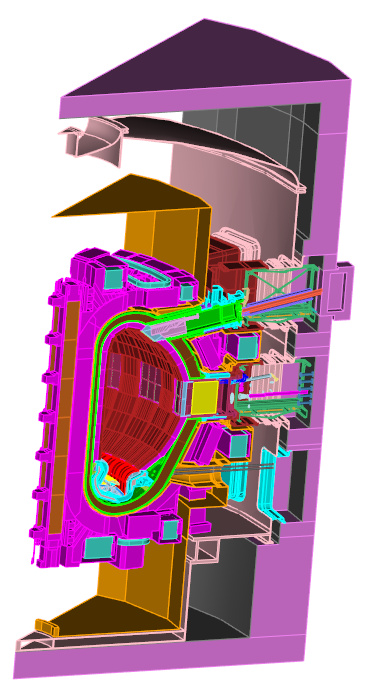
\includegraphics[scale=0.8]{../plots/cad/global.png}
  \caption{Section showing the overall model}
  \label{fig:cad_iter_global}
\end{figure}

\begin{figure}[p]
  \centering
  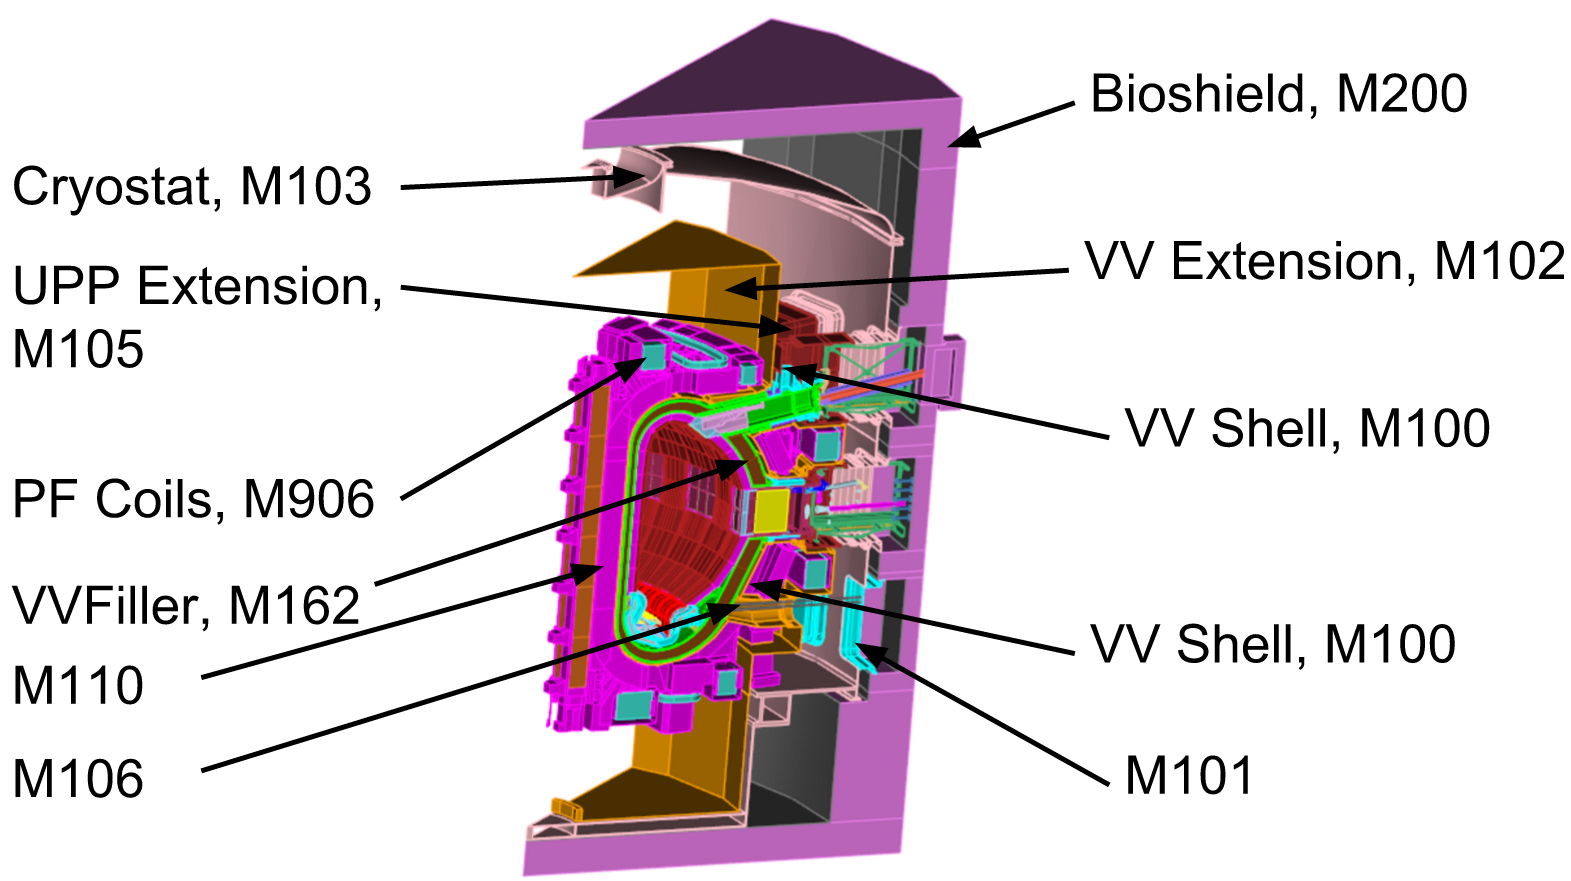
\includegraphics[scale=0.32]{../plots/cad/mats/label_1.png}
  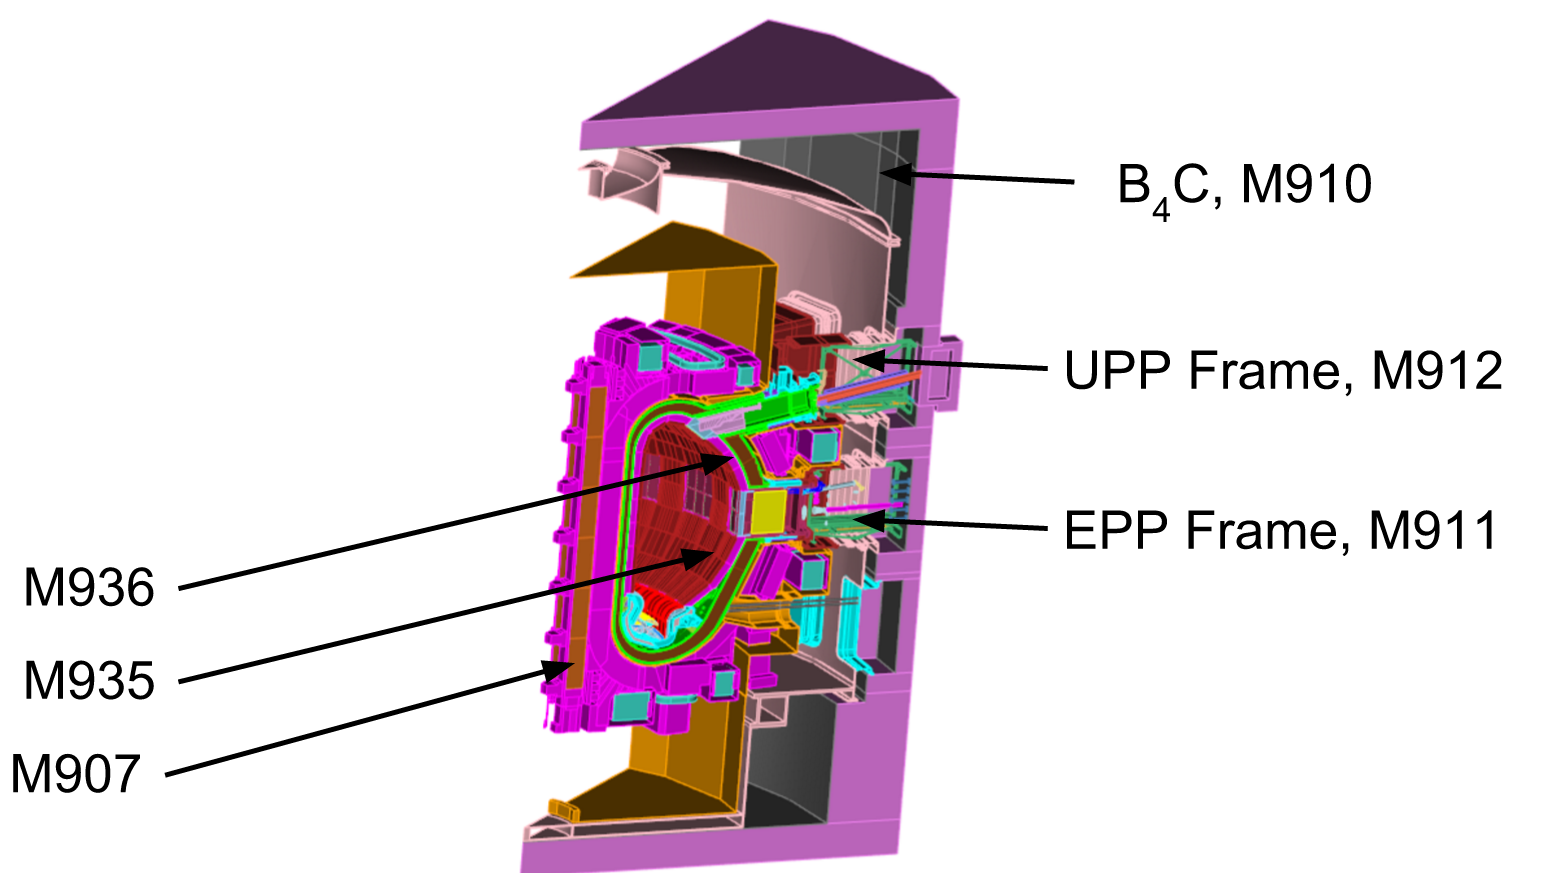
\includegraphics[scale=0.32]{../plots/cad/mats/label_2.png}
  \caption{Section some of the major tokamak materials}
  \label{fig:material_assign_1}
\end{figure}

\begin{figure}[p]
  \centering
  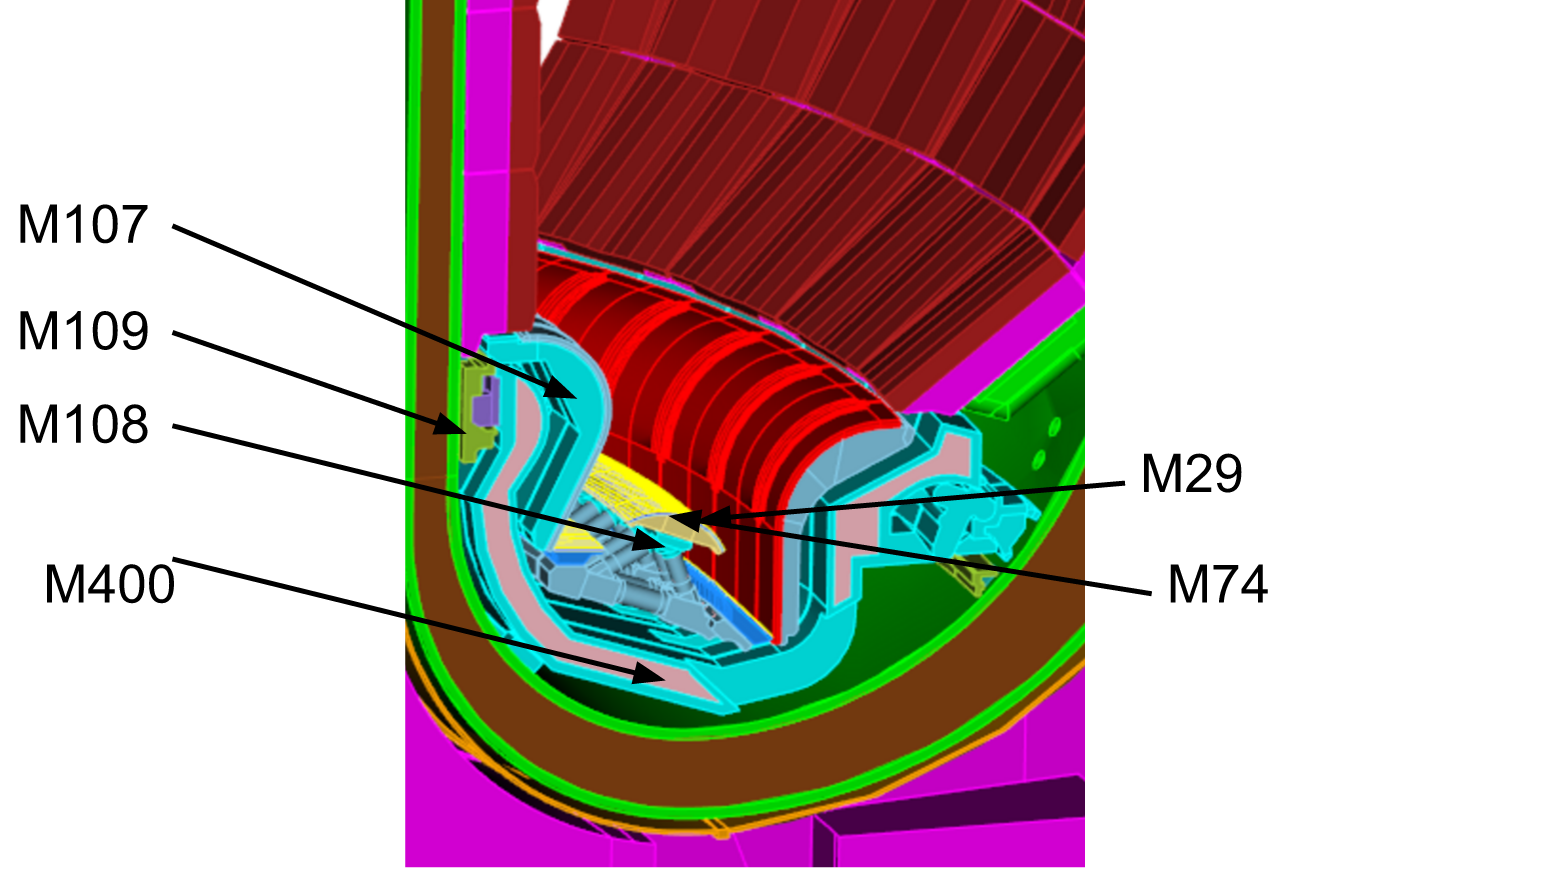
\includegraphics[scale=0.32]{../plots/cad/mats/label_3.png}
  \caption{Section some of the major tokamak materials}
  \label{fig:material_assign_2}
\end{figure}

\newpage
\clearpage
\subsubsection{Materials}
All materials in the problem originate from the Clite \gls{mcnp} model -
CLITE\textunderscore V1\textunderscore REV131031\textunderscore MOD, with the
exception of the \gls{upp}, the \gls{epp}, the
Cryopump, the blanket modules and the contents of the \gls{upi} and \gls{epi}.
The default cross section set used was \gls{fendl}-2.1, with the exception of XX
which was expanded into an isoptopic defintion and used the \gls{endf}-VIIR1
evaluation. The \gls{epp} material definitions were taken from the \gls{gepp}
\gls{mcnp} model\cite{epp_materials}. The \gls{upp} material definitions were
provided by \cite{bertalot_communication}. The Cryopump materials assignments
came from \cite{cryopump_communication}. The blanket module material
compositions were taken from the Bl-lite \gls{cad}model since the blankets were
homogenized identically in this model. The full evaluated material definitions
can be found in the Appendix.
\newpage
\subsection{Software Programs \& Validation Status}
\subsubsection{DAGMC}
The \gls{dagmc} is a toolkit developed at the \gls{uw}
designed specifically for ray tracing efficiently on complex \gls{cad} based
geometries. The \gls{dagmc} toolkit is distributed as part of \gls{moab} and
is completely open source. Input to \gls{dagmc} is a \gls{moab} mesh file
which contains the faceted representation of the \gls{cad} geometry, this
is loaded and Oriented Bounding Box (OBB) acceleration structures are built
to speed each ray fire query.
\subsubsection{DAG-MCNP5}
DAG-MCNP5 \cite{dagmc} is a version of \gls{mcnp} \cite{mcnp} where the core ray
queries (point in volume, ray fire, next volume, etc) have their \gls{mcnp}
versions replaced with the \gls{dagmc} equivlents. DAG-MCNP5 has been validated
\cite{dagmc_validation} and tested in several ITER analysis in the past.
\subsubsection{PyNE}
The \gls{pyne} \cite{Scopatz2012b} project aims to
make C++ wrapped Python-accessible library of well validated and tested
functions and capabilities available to nuclear engineers across the world.
For this project we used the following capabilities of \gls{pyne}.
\begin{itemize}
  \item{the \texttt{pyne.mesh} class to combine meshes, with an appropriate
        combined statistical error}
  \item{the \texttt{pyne.r2s} class to produce \gls{r2s} inputs and outputs}
  \item{the \texttt{pyne.alara} class to produce alara inputs}
  \item{the \texttt{pyne.mcnp} class to read \gls{mcnp} meshtal files}
\end{itemize}
\subsubsection{ALARA}
\gls{alara_c} \cite{alara} is a nuclear inventory code developed at the \gls{uw}
The unique feature of \gls{alara_c} is the way it handles the
pathways of the reactions, all of the potential pathways are accounted for and
duplicate links linearised. \gls{alara_c} is used in this analysis as the method of
producing gamma ray sources for \gls{r2s} shutdown photon calculations.
\newpage
\subsection{Solution Methodology}
\subsubsection{Neutron Transport}
The neutron transport calculations were performed using version 1.0 of DAG-MCNP5
using the source from version 1.60 of MCNP5, from the develop branch with git
checkout \texttt{e12e2a3}. The two batches of calculations were performed, one
case with the B$_4$C liner and one without.
\\
\\
The level of detail present in the faceted geometry files impacts the amount of
memory required to run the calculation, this combined with the large and
detailed weight window file and the need for 175 energy group neutron spectra
in each voxel means that the calculation requires significant memory resources,
in excess of 12 Gb per CPU. It was therefore determined that in order to perform
the neutron transport in a timely fashion given the memory requirements, this
set of simulations would be considered a good case to run using a high
throughput methodology with domain replication.
\\
\\
In this method the spatial domain of the problem is duplicated and a given
meshtally superimposed onto the geometry. Several single core simulations are
launched for that specific meshtally but the random number seed is strided in
such a way that no CPU will share the same seed with another job, this is
performed using the \texttt{rand hist=n} command in \gls{mcnp}.
\begin{figure}[ht!]
  \centering
  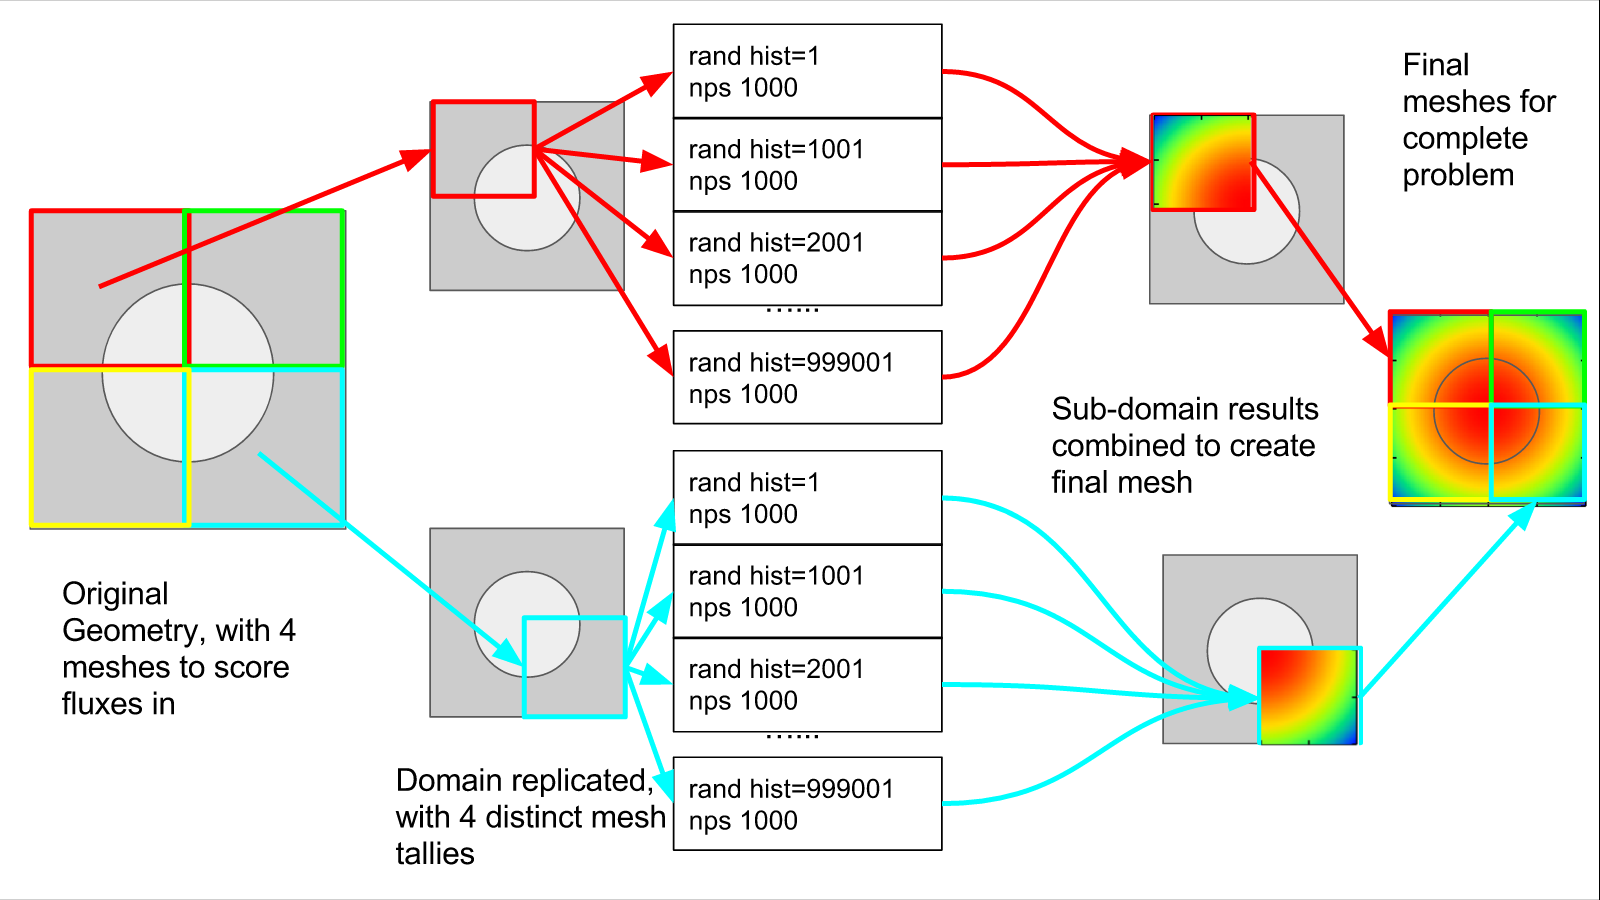
\includegraphics[scale=0.3]{../plots/method/neutron_method.png}
  \caption{The high throughput methodology, splitting a given MCNP calculation
           into smaller calculations spanning a contigious random number seed
           space}
  \label{fig:mesh_spliting}
\end{figure}
The key feature of this method is that the combined sub results are identically
equal to single MCNP calculation covering the whole original range of particles
simulated.
\begin{figure}[ht!]
  \centering
  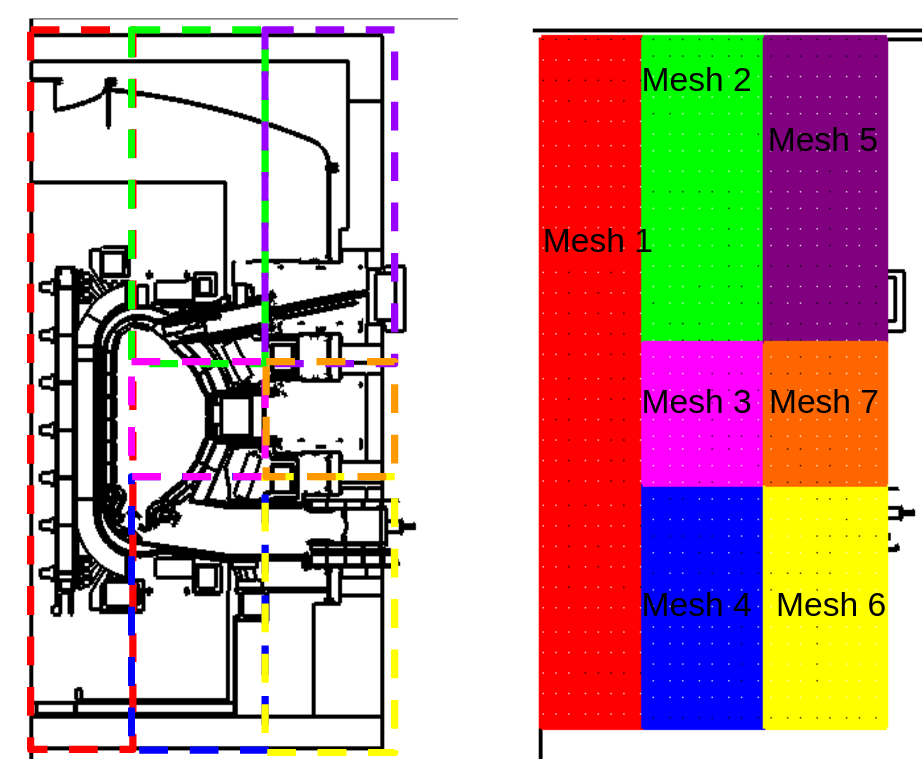
\includegraphics[scale=0.4]{../plots/transport/job_splits.png}
  \caption{The seven different mesh domains, (left) shown with some transparency
           to indicate where the major boundaries end and (right) showing the
           absolute scale of the mesh elements}
  \label{fig:mesh_domains}
\end{figure}

The calculation was split into seven calculation domains, shown in Figure
\ref{fig:mesh_domains}, which bound the regions of the problem requiring
activation. The physical size and boundaries that were used in the calculation
can be found in Table \ref{table:mesh_sizes}. With \gls{r2s} calculations there is a
subtle interplay between the size of the mesh elements and the number of mesh
elements; the larger the mesh elements the lower the statistical errors will be
for a given fixed number of particles but the mesh will conform poorly to the
geometry, and vice versa. In this calculation the maximum number of mesh
elements in a given mesh is dictated by the size that the given mesh will
occupy in memory when transferred to an \gls{alara_c}geometry. 

\begin{centering}
 \begin{table}[ht!]
  \begin{tabular}{c | c | c | c | c}
  \hline 
  Mesh & Dimension & Start position (cm) & End position (cm) & Number of bins\\
  \hline 
  \multirow{3}{*}{Mesh 1} & X & 0.0 & 500.0 & 25 \\ & Y & -250.0 & -250.0 & 25 \\
  & Z & -1500.0 & 1900.0 & 170 \\
  \hline
  \multirow{3}{*}{Mesh 2} & X & 500.0 & 1100.0 & 30 \\ & Y & -500.0 & 500.0 & 50\\
  & Z & 400.0 & 1900.0 & 75 \\
  \hline
  \multirow{3}{*}{Mesh 3} & X & 500.0 & 1100.0 & 30 \\ & Y & -500.0 & 500.0 & 50 \\
  & Z & -1500.0 & -300.0 & 60 \\
  \hline
  \multirow{3}{*}{Mesh 4} & X & 500.0 & 1100.0 & 30 \\ & Y & -500.0 & 500.0 & 50 \\
  & Z & -300.0 & 400.0 & 35 \\
  \hline
  \multirow{3}{*}{Mesh 5} & X & 1100.0 & 1700.0 & 30 \\ & Y & -600.0 & 600.0 & 60 \\
  & Z & -1500.0 & -300.0 & 60 \\
  \hline
  \multirow{3}{*}{Mesh 6} & X & 1100.0 & 1700.0 & 60 \\ & Y & -600.0 & 600.0 & 60 \\
  & Z & 400.0 & 1900.0 & 75\\
  \hline
  \multirow{3}{*}{Mesh 7} & X & 1100.0 & 1700.0 & 30 \\ & Y & -600.0 & 600.0 & 60 \\
  & Z & -300.0 & 400.0 & 36 
  \end{tabular}
 \caption{The meshes used in the problem, their start and end coordinate and
          number of divisions}
 \label{table:mesh_sizes}
 \end{table}
\end{centering}
\subsubsection{Activation}
The activation calculations are performed using the spatially dependent neutron
spectra determined in the previous step. The activation calculations proceed as
a set of standard mesh based \gls{r2s} calculations typically proceed since the 
meshes do not overlap, this is shown scematically in Figure
\ref{fig:activation_method}
\begin{figure}[ht!]
  \centering
  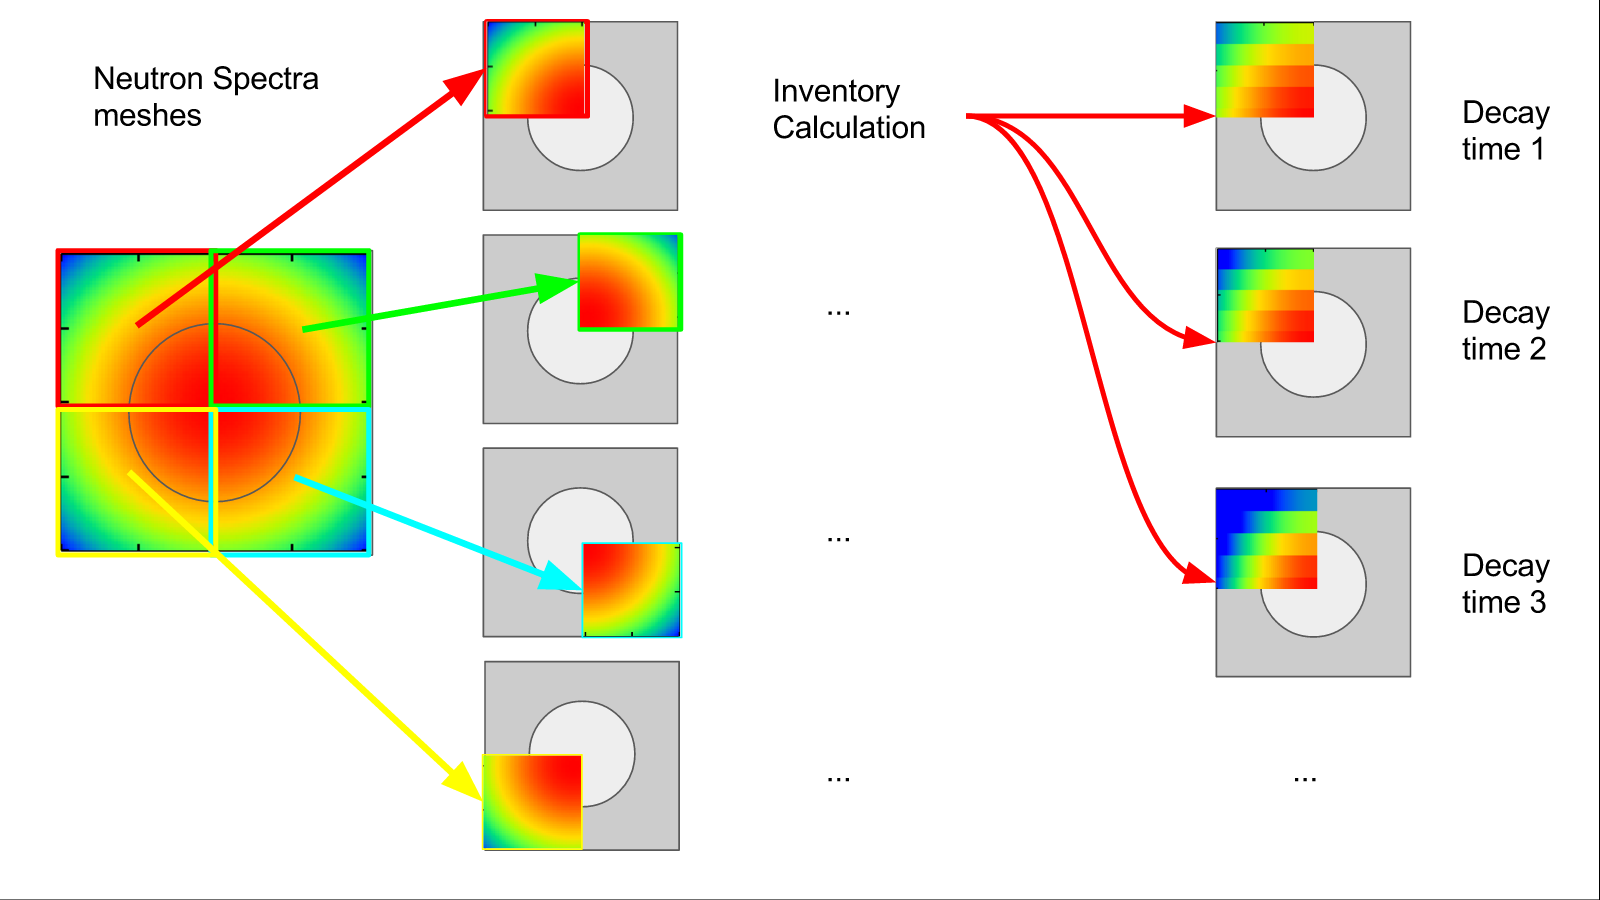
\includegraphics[scale=0.3]{../plots/method/activation_method.png}
  \caption{The methodology of having several activation meshes distributed
           across a given problem to generate several spatially discrete
           decay sources}
  \label{fig:activation_method}
\end{figure}
The geometery under each voxel in the mesh is queried to 
determine the average material composition by volume fraction, a material 
description is developed and recorded for running in an inventory code. In the 
case of \texttt{pyne.r2s} a full \gls{alara_c} input deck is produced which can
then be executed and the final shutdown photon sources produced. From a single
inventory calculation the decay photon sources for all the subsequent decay
times can be generated.  
\subsubsection{Photon Transport}
The photon transport proceeds using the same computational model as in the 
neutron calculation, with the exception the photon source and appropriate 
normalisation is determined using the activation step. The calculation is then
performed, but each photon transport will use a common result mesh for each 
calculation, and therefore, since each photon source is determined for a 
specific non overlapping region of the geometry the final result is the 
summation of each mesh, with the statistical error propagated appropriately.
\subsection{Software Risk Assesment}
\clearpage
\newpage
\section{Assumptions and Engineering Judgements}
\subsection{Neutron Source}
As used in typical ITER analysis the reference ITER neutron source with
reflecting boundary conditions is assumed to adequately represent the
true 360$^{\circ}$ neutron source. The ITER supplied MCNP SDEF was used
completely unmodified. The onload neutron data is used un-normalised
in the \gls{r2s} calculation since the neutron source normalisation is scaled
depending on average power for the pulse being modelled. However for reference,
the highest power used in the activation calculation was 500 MW, which is
equivlent to 1.98$\times$10$^{18}$ neutrons per second in the 40$^{\circ}$
sector. Given that this is the IO approved neutron source description, it is
assumed to be adequate for this simulation.
\subsection{Irradiation Scenario}
The irradiation scenario used in this work was the MDRG-2, shown in Table
\ref{tab:irrad_scenario} scenario as opposed to the typical SA-2 scenario.
The MDRG-2 scenario is more aggressive in overall fluence than the SA-2
scenario, representing a full ITER lifetime as opposed to 2 operation
cycles of the SA-2 scenario.
\begin{table}[ht!]
   \begin{tabular}{| l | c |}
      \hline 
      Irradiation Period & Fractional Strength \\
      \hline
      5 Years & 0.0095 \\
      1 Year  & 0.0127 \\
      1 Year  & 0.0190 \\
      1 Year  & 0.0317 \\
      1 Year  & 0.0380 \\
      1 Year  & 0.0380 \\
      6 Days  & 0.1929 \\
      1 Year  & 0.0380 \\
      \cellcolor{blue!25} 400 Seconds & 1.0000 \\
      \cellcolor{blue!25}1673.6 Seconds & 0.0000 \\
      400 Seconds & 1.0000 \\
      \hline
\end{tabular}
\caption{The table shows the MDRG-2 scenario for irradiation, note the
         cells in \textcolor{blue!25}{blue} are repeated 249 times}
\label{tab:irrad_scenario}
\end{table}
It is assumed that the longer fluence operation will lead to greater accumulated
radionuclides, which should provide a conservative estimate of shutdown photon
doserate.
\\
\\
In this report time periods following machine shutdown are of interest,
1.0$\times$10$^5$ s, 1.0$\times$10$^6$ s and 1.0$\times$10$^6$ s, approximately
corresponding to 27 hours, 14 days, and 116 days post shutdown.
\subsection{Geometry}
The geometry used in this simulation was collected from a number of sources,
some models were generated directly from CAD drawings supplied by the
drawing office of US ITER and the IO, some were intermediate CAD files produced
as part of other simulations, and some were generated by \gls{uw} to meet a
percieved deficiency in the file. Irrespective of this, the \gls{dagmc} method
allows the exact respresentation of the underlying CAD to be used without
approximation.
\\
\\
The geometry is defined starting at the centre column (x = 0.0 cm) and ends
beyond the bioshield (x = 1800 cm), truncation of details realtive to the full
ITER device CAD model begins on the port cell side of the bioshield plugs,
results beyond the bioshield should therefore be not be used for any
analysis purposes. 
\subsection{Variance Reduction}
The weight window parameters were generated using the \gls{ornl} code
\gls{advantg}, specifically using DAG-\gls{advantg}, which allows a
\gls{dagmc} geometry to be read and the geometry and material data handed off to
Denovo. The weight windows used for the problem are shown below in Figure
\ref{fig:wwinp}. The weight windows were produced using the \gls{fwcadis},
which attempts to produce a weight window map which tries to get particles
everywhere int the model, as opposed to \gls{cadis} for example, which
attempts to get results to a small number of specific regions.
\begin{figure}[ht!]
  \centering
  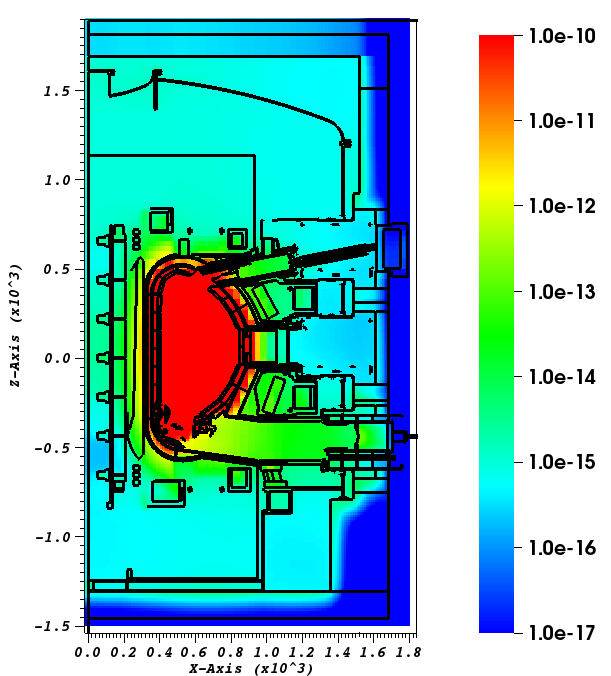
\includegraphics[scale=0.4]{../plots/wwinp/wwinp_y0.png}
  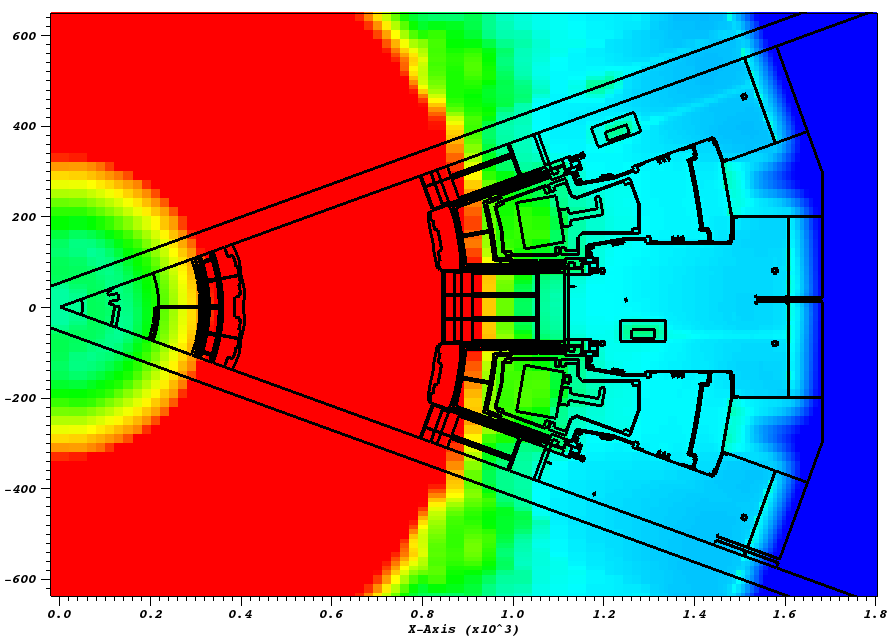
\includegraphics[scale=0.3]{../plots/wwinp/wwinp_z0.png}
  \caption{Slices through the \gls{advantg} produced weight window through y =
  0.0 cm and through z = 0.0 cm}
  \label{fig:wwinp}
\end{figure}
Several artifacts are worthy of note, despite being a deterministic code Denovo
has handled the streaming of neutrons along the divertor duct well as shown in
left hand image of Figure \ref{fig:wwinp}. The overall span of the weight window
is seven orders of magnitude, which is largely proportional to the neutron
attenuation from the plasma to the port interspace, previous calculations put
the attenuation in the range of 6 to 8 orders of magnitude. There is some
evidence of ray effects in the weight window solution in the right hand image
of Figure \ref{fig:wwinp} due to the neutron attenuation of some \gls{epi}
shielding around the diagnostic equipment, but this is small deviation in an
otherwise reasonable solution.
\\
\\
It should be noted that \gls{ornl} specifically developed the 360$^{\circ}$
rotation feature for DAG-\gls{advantg} that allows rotationally symmetric
bodies, which is the reason for the weight window values beyond the
40$^{\circ}$ sector.
\subsection{Materials and Nuclear Data}
\subsubsection{Materials}
The full description of material contents can be found in the Appendix. The 
origin of each material is desribed in Table \ref{tab:material_origin}. 

\begin{centering}
 \begin{longtable}[ht!]{ p{0.2\textwidth} | p{0.3\textwidth} | p{0.3\textwidth} }
  \hline 
  Material Number & Description & Origin \\
  \hline
  M29  & &  CLITE V1 \\
  M74  & &  CLITE V1 \\
  M100  & &  CLITE V1 \\
  M101  & &  CLITE V1 \\
  M102  & &  CLITE V1 \\
  M103  & &  CLITE V1 \\
  M104  & &  CLITE V1 \\
  M105  & &  CLITE V1 \\
  M106  & &  CLITE V1 \\
  M107  & &  CLITE V1 \\
  M108  & &  CLITE V1 \\
  M109  & &  CLITE V1 \\
  M110  & &  CLITE V1 \\
  M111  & &  CLITE V1 \\
  M162  & &  CLITE V1 \\
  M170  & &  CLITE V1 \\
  M200  & &  CLITE V1 \\
  M303  & &  CLITE V1 \\
  M400  & &  CLITE V1 \\
  M601  & &  CLITE V1 \\
  M602  & &  CLITE V1 \\
  M603  & &  CLITE V1 \\
  M611  & &  CLITE V1 \\
  M613  & &  CLITE V1 \\
  M621  & &  CLITE V1 \\
  M622  & &  CLITE V1 \\
  M623  & &  CLITE V1 \\
  M631  & &  CLITE V1 \\
  M906  & &  CLITE V1 \\
  M907  & &  CLITE V1 \\
  M908  & &  CLITE V1 \\
  M910 & B$_4$C & Bespoke  \\
  M911 & Al T6061 & Bespoke  \\
  M912 & Al T6061 & Bespoke  \\
  M913 & Copy M100 & CLITE V1\\
  M914 & Copy M100 & CLITE V1\\
  M915 & Copy M910 & Bespoke \\
  M916 & Copy M100 & CLITE V1\\
  M917 & Cryopipes & \cite{neutr anal materials}\\
  M918 & Copy M100 & CLITE V1 \\
  M920 & Copy M100 & CLITE V1 \\
  M921 & Copy M100 & CLITE V1 \\
  M922 & Copy M100 & CLITE V1 \\
  M923 & Copy M100 & CLITE V1 \\
  M924 & Copy M100 & CLITE V1 \\
  M925 & Copy M100 & CLITE V1 \\
  M926 & Copy M100 - Frame Wheels & \cite{neutr_anal_materials}\\
  M927 & Copy M100 - Frame Wheels Drive & \cite{neutr_anal_materials}\\
  M928 & Copy M100 - Port Plug Frame & \cite{neutr_anal_materials}\\
  M929 & Copy M100 - Port Plug Pipes & \cite{neutr_anal_materials}\\
  M930 & Copy M100 & \cite{neutr_anal_materials}\\
  M931 & M100:0.7 M400:0.3 & \cite{neutr_anal_materials}\\
  M932 & M100:0.9 M400:0.1 & \cite{neutr_anal_materials}\\
  M933 & M100:0.9 M400:0.1 & \cite{neutr_anal_materials}\\
  M934 & M100:0.97 M400:0.03 & \cite{neutr_anal_materials}\\
  M937 & Copy M100 & \cite{neutr_anal_materials}\\
  M938 & Copy M100 & \cite{neutr_anal_materials}\\
  M939 & Copy M100 & \cite{neutr_anal_materials}\\
  M935 & First Wall & BL-lite \\
  M936 & First Wall & BL-lite \\
  M940 & Copy M100 & Diagnostics MCNP Model \\
  M941 & Copy M100 & Diagnostics MCNP Model \\
  M942 & Copy M100 & Diagnostics MCNP Model \\
  M943 & Copy M100 & Diagnostics MCNP Model \\
  M944 & EPP Drawers & Diagnostics MCNP Model \\
  M945 & EPP Contents & Diagnostics MCNP Model \\
  M946 & EPP Chunks & Diagnostics MCNP Model \\
 \caption{Table showing the origin of the material descriptions used}
 \label{tab:material_origin}
 \end{longtable}
\end{centering}

\subsubsection*{Nuclear Data}
Neutron Data - The neutron transport data used was \gls{fendl}-2.1/MC, as 
recommended by \gls{io} for ITER analysis. 
\\
\\
Activation Data - The activation data used was \gls{fendl}-3.0/A.
\\
\\
Photon Data - The standard photon data supplied with \gls{mcnp}5 mcplib04 was 
used. This data ultimately falls back onto \gls{endf}/B-VI release 8 photoatomic
data.
\subsection{Transport Software}
\gls{mcnp}
\subsection{Activation Software}
\gls{alara_c}
\newpage
\clearpage
\section{Neutron Transport Results and Conclusions}
Using the methodology shown in Section \ref{section:method}, the neutron meshes
were split into 7 calculations. These jobs were submited to the \gls{uw}
\gls{chtc} system in batches of 200
for each mesh, with seven meshes used to determine the neutron flux, making a
total of 2800 individual \gls{mcnp} simulations. These results were then
combined using \gls{pyne} to result in the statistically averaged final results.
Intially calculations were batched into groups of $5\times10^7$ particles per
batch, however these calculations did not finish in a timely enough manner and
were instead reduced to groups of $5\times10^6$ particles per batch. With the
smaller batching system calculations did finish, however, only 10\% of all
calculations for each mesh finished, but this represents $5\times10^7$ total
source histories for each mesh.
\\
\\
\subsection{Without the B4C Liner}
The baseline results represent a standard C-lite model since there is no B$_4$C
liner present, however relative to the standard C-lite native \gls{mcnp} model
there is much more equipment present in the \gls{upi} \& \gls{epi}, and
the divertor pumping port is unplugged. The open pumping port specifically
leads to higher neutron fluxes beyond the vacuum vessel.
\begin{figure}[ht!]
  \centering
  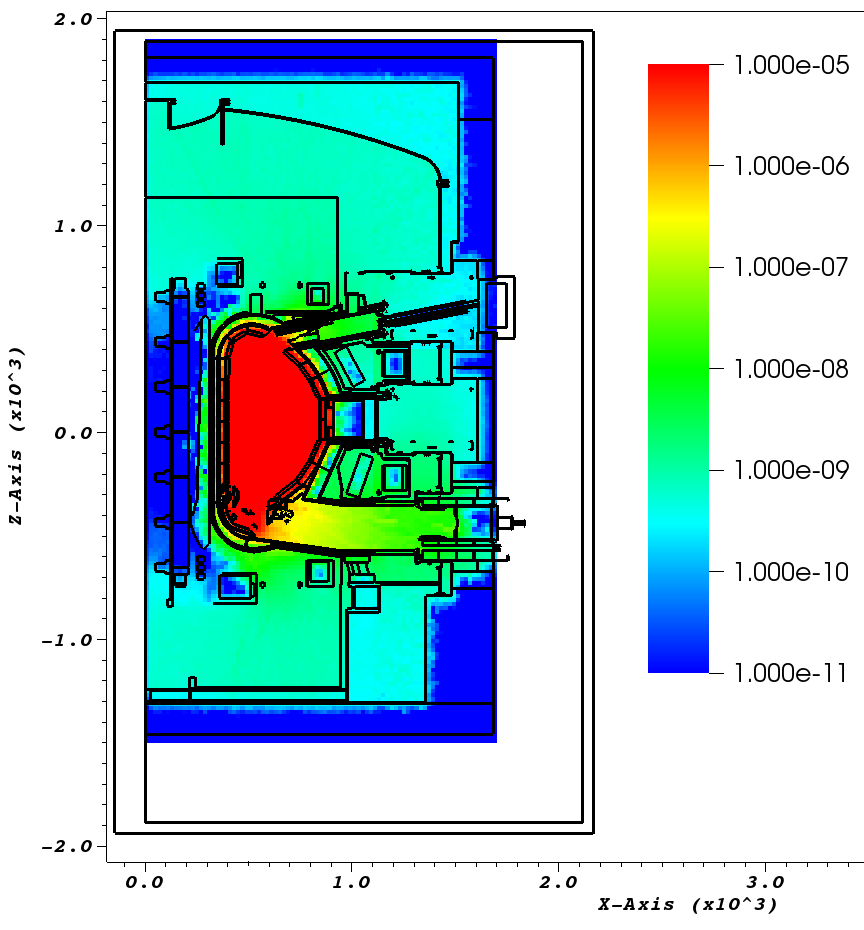
\includegraphics[scale=0.35]{../plots/neutron/nob4c/y_0.png}
  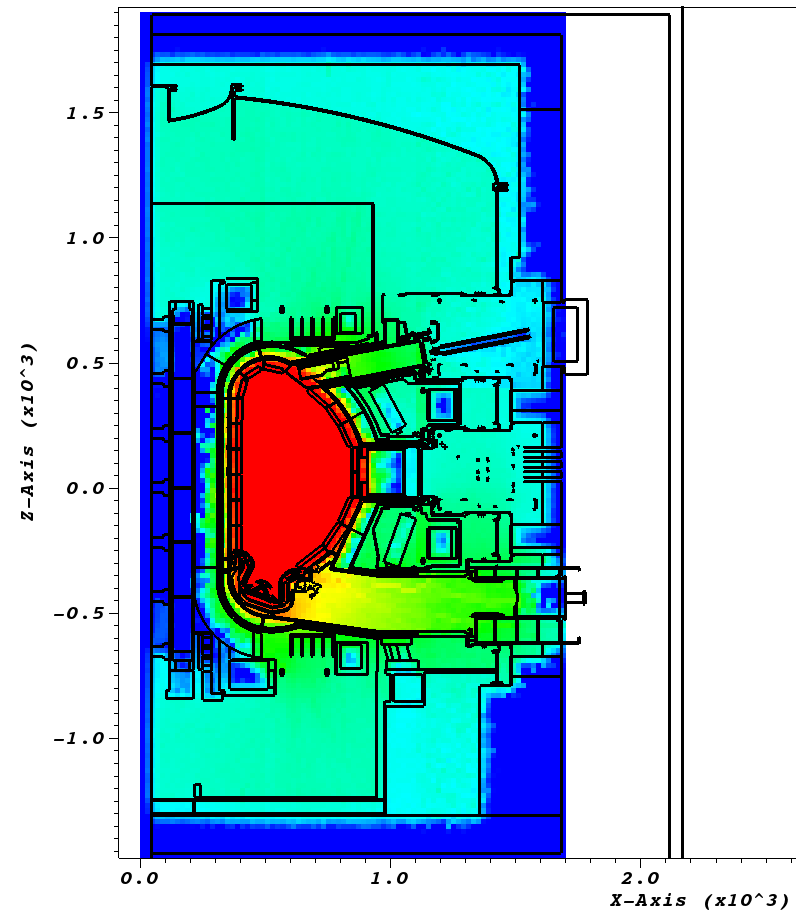
\includegraphics[scale=0.35]{../plots/neutron/nob4c/y_-17.png}
  \caption{Slices through the total neutron flux (n cm$^{-2}$ src$^{-1}$)
  y = -17.0 cm and through z = 0.0 cm}
  \label{fig:wwinp}
\end{figure}
\begin{figure}[ht!]
  \centering
  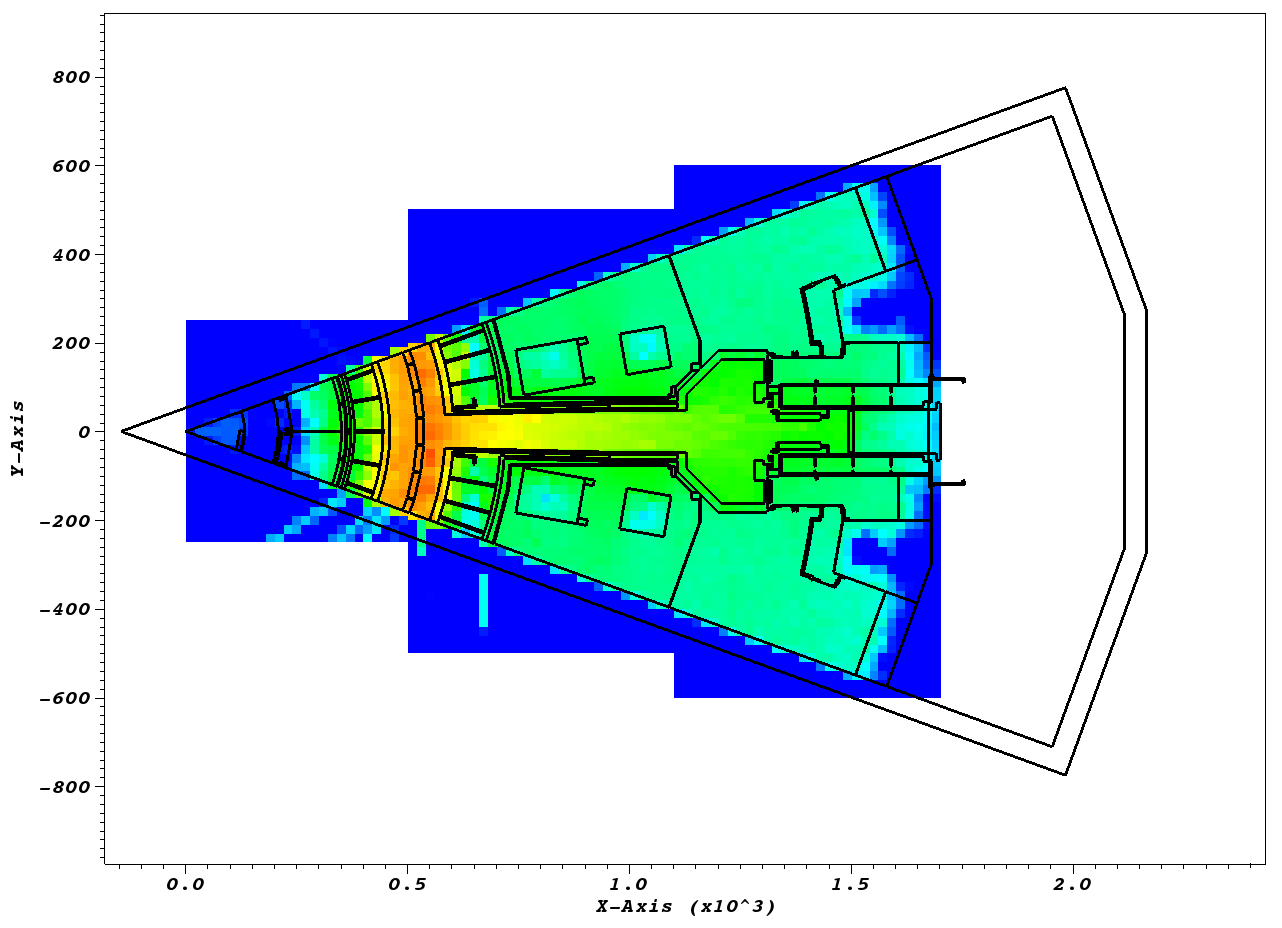
\includegraphics[scale=0.27]{../plots/neutron/nob4c/z_-500.png}
  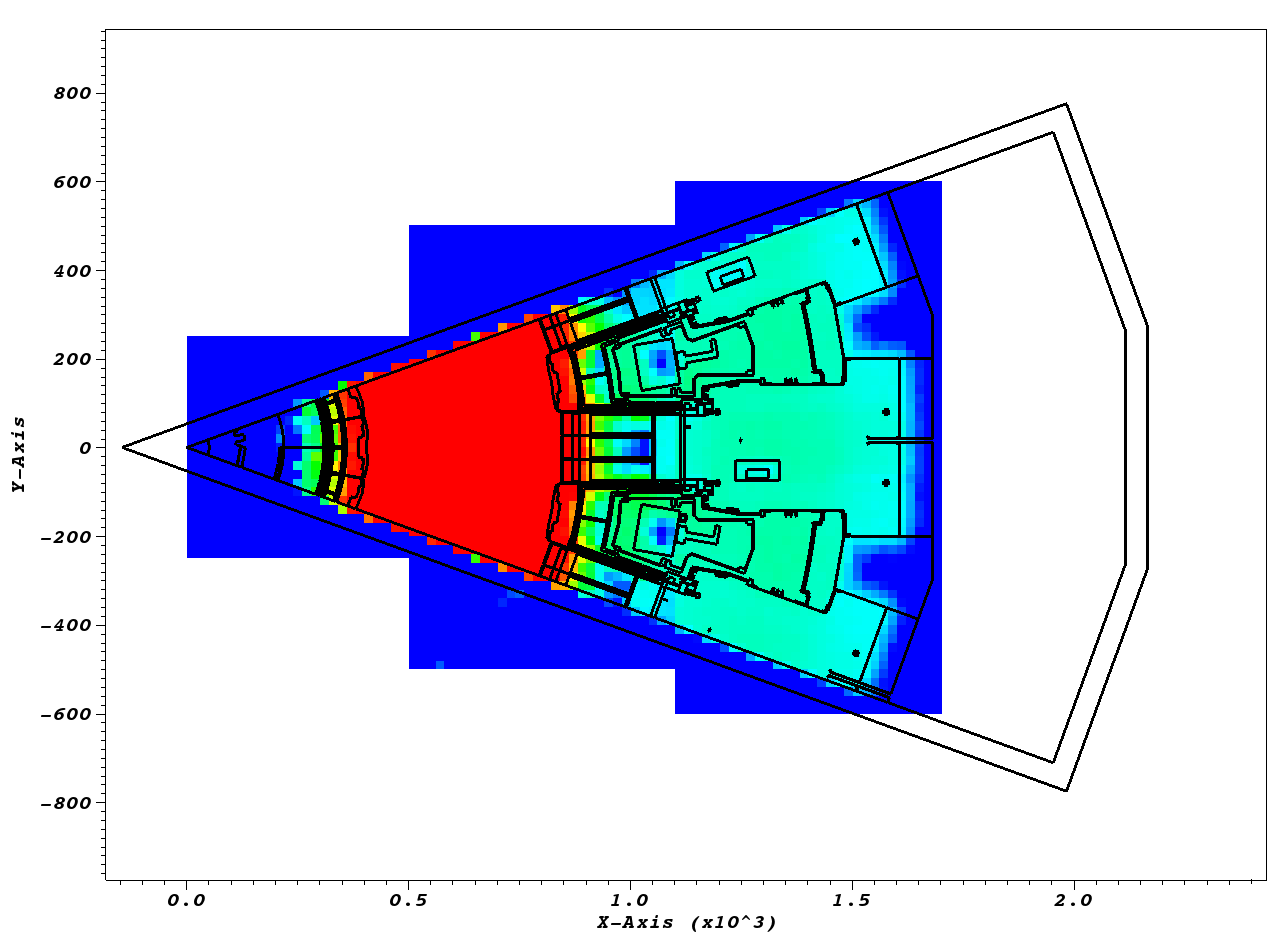
\includegraphics[scale=0.27]{../plots/neutron/nob4c/z_0.png}       
  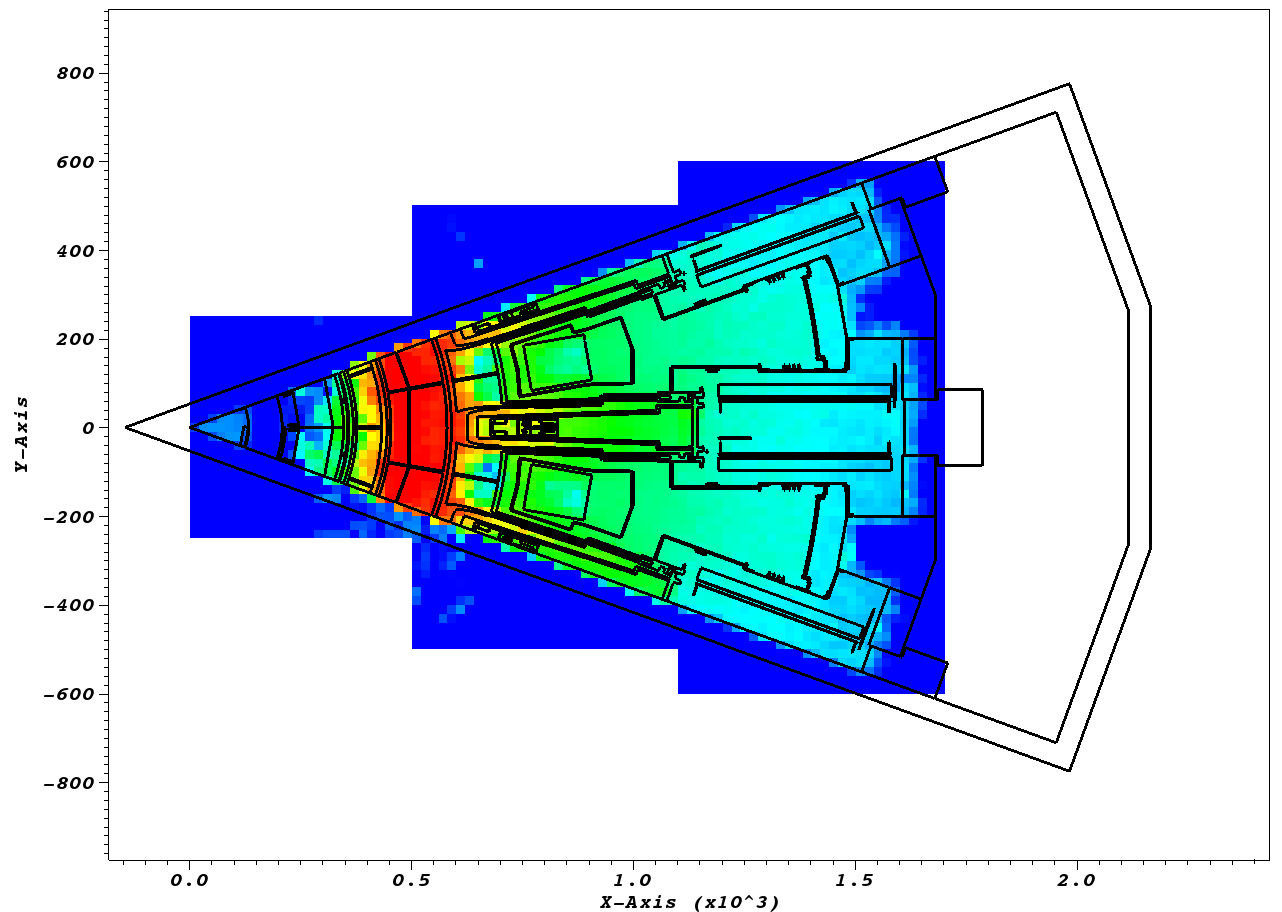
\includegraphics[scale=0.27]{../plots/neutron/nob4c/z_500.png}
  \caption{Slices through the total neutron flux (n cm$^{-2}$ src$^{-1}$)
  z = -500.0 cm and through z = 500.0 cm}
  \label{fig:wwinp}
\end{figure}
\newpage
\clearpage
\subsection{Including the B4C Liner}
These results represent a standard C-lite model with improved B$_4$C liner,
however relative to the standard C-lite native \gls{mcnp} model there is much more
equipment present in the port inspaces (both upper and lower), and the divertor
pumping port is unplugged. 
\begin{figure}[ht!]
  \centering
  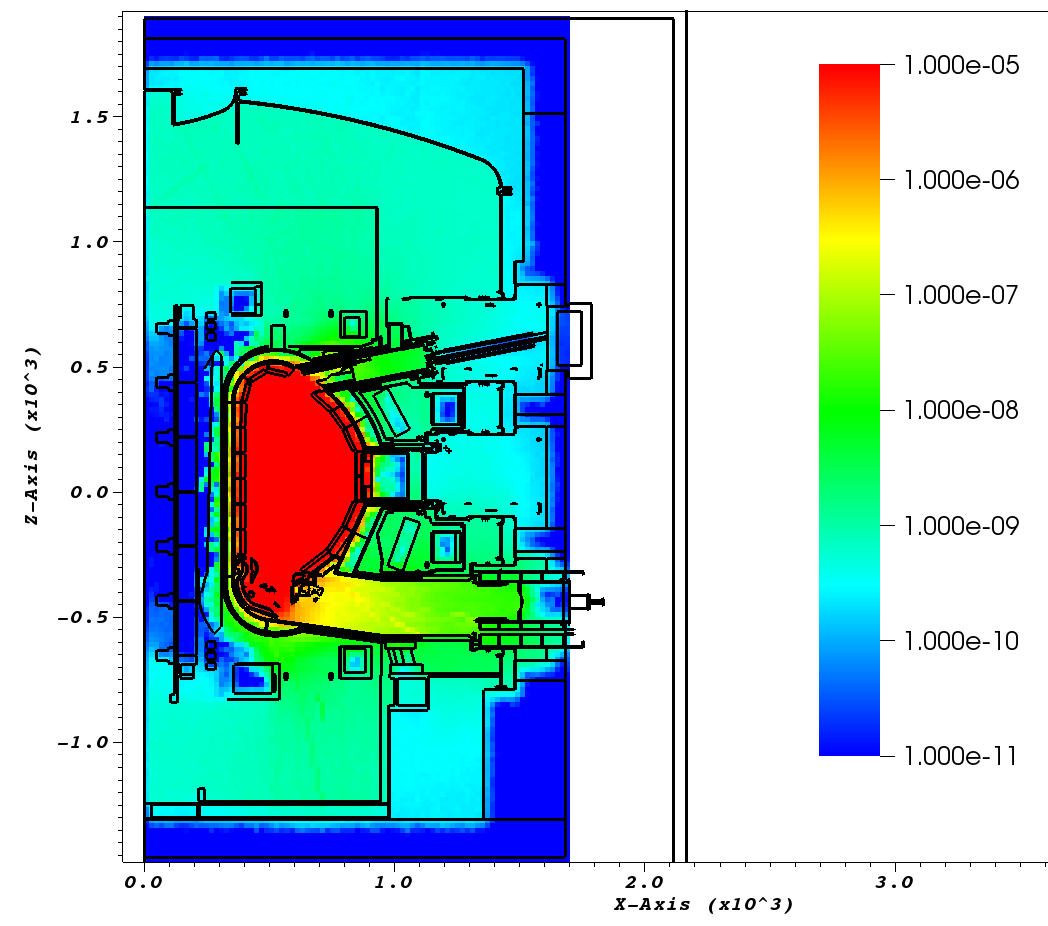
\includegraphics[scale=0.35]{../plots/neutron/b4c/flux_y0.png}     
  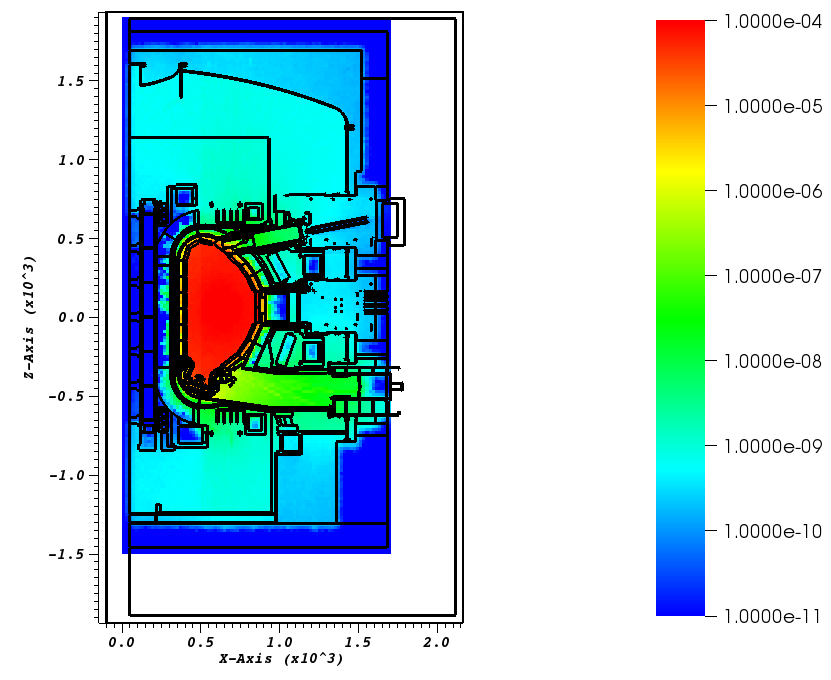
\includegraphics[scale=0.35]{../plots/neutron/b4c/flux_y-17.png}
  \caption{Slices through the total neutron flux (n cm$^{-2}$ src$^{-1}$)
           y = -17.0 cm and through z = 0.0 cm}
  \label{fig:wwinp}
\end{figure}
\begin{figure}[ht!]
  \centering
  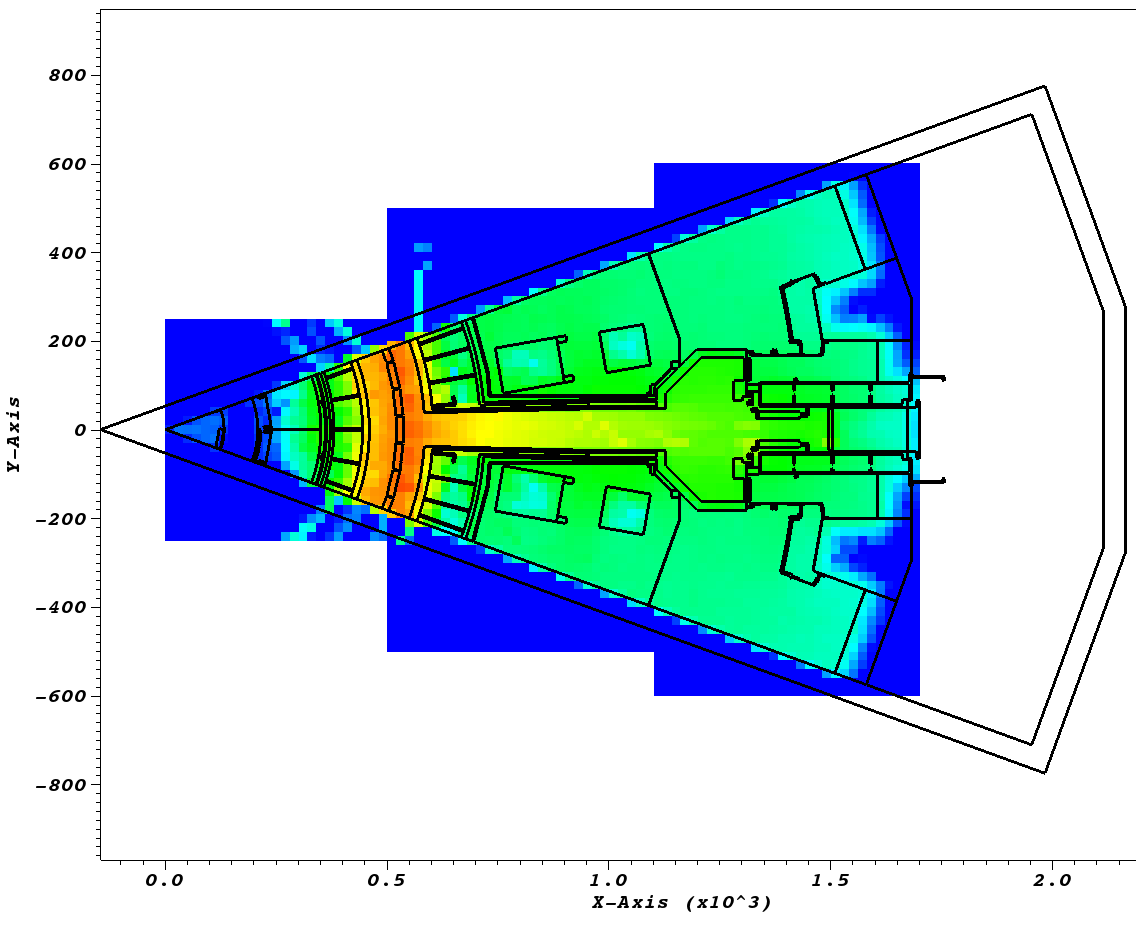
\includegraphics[scale=0.27]{../plots/neutron/b4c/flux_z-500.png}
  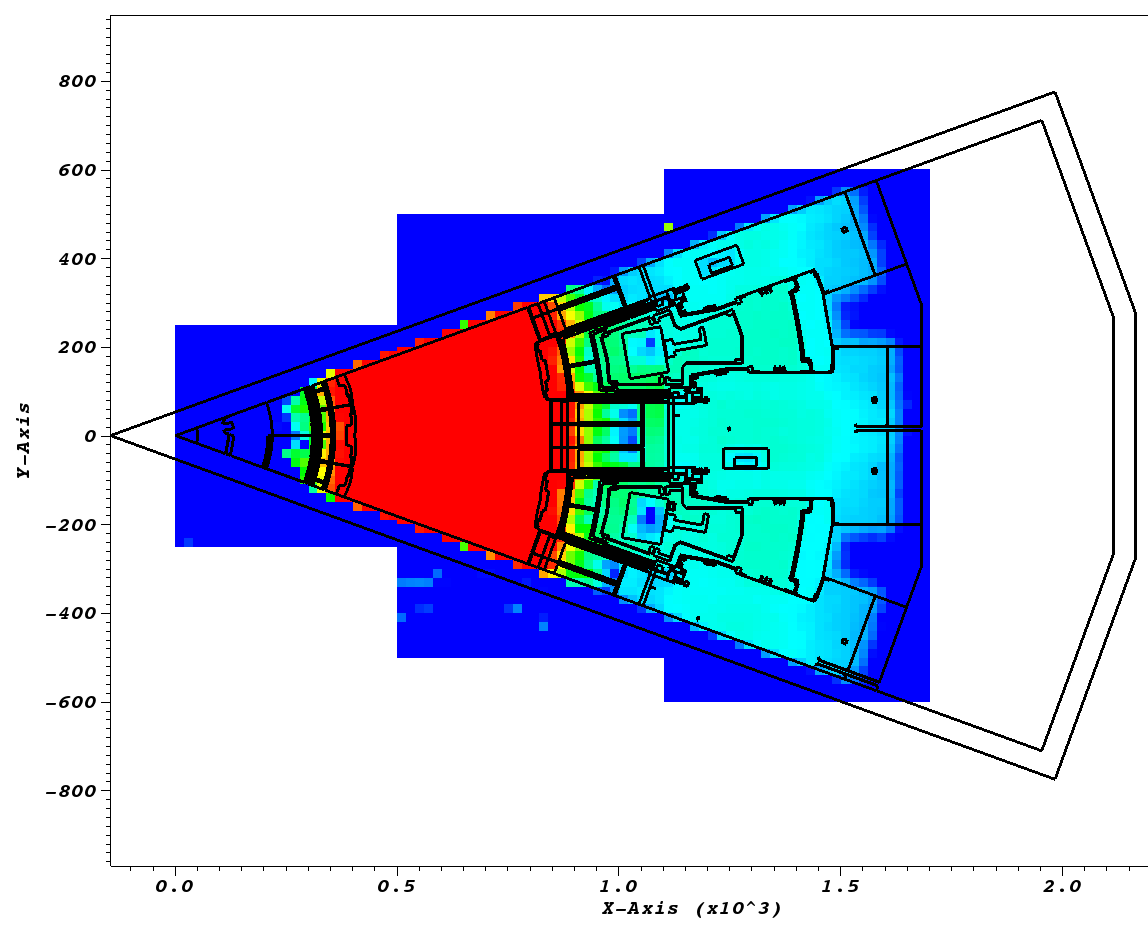
\includegraphics[scale=0.27]{../plots/neutron/b4c/flux_z0.png}       
  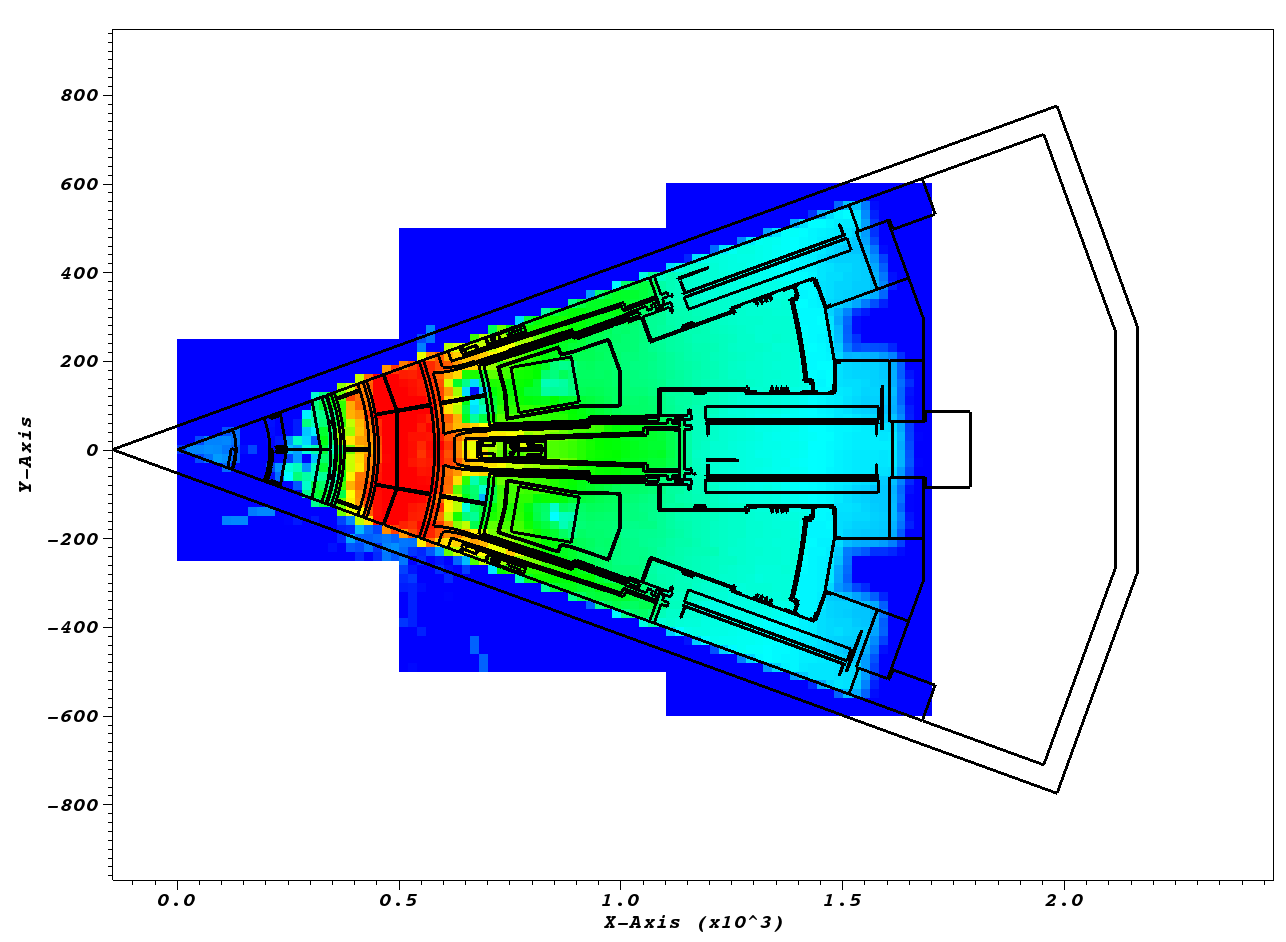
\includegraphics[scale=0.27]{../plots/neutron/b4c/flux_z500.png}
  \caption{Slices through the total neutron flux (n cm$^{-2}$ src$^{-1}$)
           z = -500.0 cm and through z = 500.0 cm}
  \label{fig:wwinp}
\end{figure}
\subsection{Conclusion}
The final calulcations represent only around 10\% of the overall requested
runtime, this is mostly due to calculations not completing with the 3 day
allotted runtime on CHTC, the reason being that is seems the requested VR
parameters were too extreme resulting in severe oversplitting of particles.
This has been noticed to occur in several previous challenging attenuating
geometries and has been attributed to so called long histories. The long history
problem requires an ultimate solution beyond the scope of this report, but
perhaps solutions like that already underway at UW-Madison \& \gls{ornl}; GT-CADIS
\& MS-CADIS respectively.
\newpage
\clearpage

\section{Neutron Activation Results and Conclusions}
The \gls{r2s} shutdown dose rate calculations were performed using the pyne.r2s
methods found \gls{pyne}. The setup scripts produce \gls{alara_c} inputs and the neutron
activation calculations were performed using \gls{alara_c} 2.9.1RC which used the
\gls{fendl}-3.0/A activation cross sections. 
\subsection{Including the B4C Liner}
\subsection{Without the B4C Liner}
\subsection{Conclusion}
\newpage
\section{Shutdown Photon Doserates Results and Conclusions}
The shutdown photon sources were developed in several seperate meshes and
therefore any individual mesh does not represent the entire problem. The
results of the previous \gls{alara_c} calculations are then processed further to make
shutdown sources to be read into a sampling subroutine (also distributed with
\gls{pyne}) Each source is run independently, and the photon dose is recorded on a
mesh common to each photon calculation and then the meshes summed together to
create the final result. The final mesh has a uniform size of side 2 cm striding
from x = {0,1500}, y = {-500,500}, z = {-1900,1500} cm. The meshes used the
\gls{icrp}-74 dose response coeffiecients as a dose multiplier as recommended in
\cite{iter_sdr_coeffs}.
\subsection{Decay time 1 - 1.$\times$10$^5$ s}
\subsection{Decay time 2 - 1.$\times$10$^6$ s}
\subsection{Decay time 3 - 1.$\times$10$^7$ s}
\subsection{Conclusion}
It is clear from Figures XXX that the shutdown photon doserate in the port
interspaces is affected by the addition of boron carbide to the plasma side
surface of the bioshield. The reason for the this is significantly degraded
thermal flux which impacts the inportance of (n,$\gamma$) reactions and also
the transport of neutrons back from the bioshield. The true benefit appears
only to be very close to the B$_4$C layer, where is reduces the activation of
steel componenets near to the bioshield, those components away from the
bioshield appear to have their activation dominated by the neutron tranported
via long paths around other ports, known as cross talk.
\section{Calculation Details}
\subsection{Neutron Transport}
\subsubsection{Baseline}
\subsubsection{With B$_4$C}
\subsection{Activation Calculations}
\subsubsection{Baseline}
\subsubsection{With B$_4$C}
\subsection{Photon Transport}
\subsubsection{Baseline}
\subsubsection{With B$_4$C}

\section{Acceptance Criteria}
\section{Lessons learned and future work}
\section{Acknowledgements}

\bibliographystyle{unsrt}
\bibliography{bibliography}
\newpage
\section{Appendix}
\begin{centering}
\begin{table}[ht!]
\begin{tabular}{l | c}
\hline
Nuclide & Atom Fraction\\
\hline
H1 & 6.997078e-04\\
H2 & 1.608276e-07\\
B10 & 1.831598e-06\\
B11 & 8.106036e-06\\
C12 & 2.946747e-04\\
N14 & 6.928888e-04\\
N15 & 2.769410e-06\\
O16 & 5.539577e-03\\
Si28 & 4.564952e-03\\
Si29 & 2.400762e-04\\
Si30 & 1.637057e-04\\
P31 & 2.484376e-04\\
S & 9.937764e-05\\
Ti46 & 7.870667e-05\\
Ti47 & 7.252245e-05\\
Ti48 & 7.335356e-04\\
Ti49 & 5.497666e-05\\
Ti50 & 5.371156e-05\\
Cr50 & 7.258372e-03\\
Cr52 & 1.455608e-01\\
Cr53 & 1.682310e-02\\
Cr54 & 4.266560e-03\\
Mn55 & 1.788766e-02\\
Fe54 & 3.637981e-02\\
Fe56 & 5.922114e-01\\
Fe57 & 1.392136e-02\\
Fe58 & 1.885133e-03\\
Co59 & 4.968802e-04\\
Ni58 & 8.180318e-02\\
Ni60 & 3.259580e-02\\
Ni61 & 1.440563e-03\\
Ni62 & 4.668329e-03\\
Ni64 & 1.227273e-03\\
Cu63 & 2.042160e-03\\
Cu65 & 9.391214e-04\\
Nb93 & 9.937617e-05\\
Mo92 & 3.532189e-03\\
Mo94 & 2.249541e-03\\
Mo95 & 3.912899e-03\\
Mo96 & 4.142835e-03\\
Mo97 & 2.396706e-03\\
Mo98 & 6.118223e-03\\
Mo100 & 2.491646e-03\\
Ta181 & 9.937573e-05
\end{tabular}
\caption{Table showing the isotopic description of material EPP3L}
\label{table:material_EPP3L}
\end{table}
\clearpage
\begin{table}[ht!]
\begin{tabular}{l | c}
\hline
Nuclide & Mass Fraction\\
\hline
He4 & 3.355146e-03\\
B10 & 1.802792e-04\\
B11 & 7.978553e-04\\
C12 & 1.970612e-04\\
N14 & 9.160305e-04\\
N15 & 3.624343e-06\\
O16 & 1.378506e-02\\
Al27 & 6.199031e-04\\
Si28 & 1.295973e-02\\
Si29 & 6.826361e-04\\
Si30 & 4.652330e-04\\
P31 & 2.955888e-04\\
S & 1.970642e-04\\
K & 7.614452e-05\\
Ti46 & 1.096136e-04\\
Ti47 & 1.010008e-04\\
Ti48 & 1.022010e-03\\
Ti49 & 7.656520e-05\\
Ti50 & 7.480316e-05\\
V & 2.627356e-05\\
Cr50 & 4.743983e-03\\
Cr52 & 9.513602e-02\\
Cr53 & 1.099539e-02\\
Cr54 & 2.788589e-03\\
Mn55 & 1.313740e-02\\
Fe54 & 2.407534e-02\\
Fe56 & 3.919107e-01\\
Fe57 & 9.212806e-03\\
Fe58 & 1.247545e-03\\
Co59 & 3.284351e-04\\
Ni58 & 5.296795e-02\\
Ni60 & 2.110594e-02\\
Ni61 & 9.327718e-04\\
Ni62 & 3.022769e-03\\
Ni64 & 7.946654e-04\\
Cu63 & 1.898430e-01\\
Cu65 & 8.730242e-02\\
Zr & 1.313594e-05\\
Nb93 & 2.401275e-02\\
Mo92 & 2.334761e-03\\
Mo94 & 1.486929e-03\\
Mo95 & 2.586387e-03\\
Mo96 & 2.738387e-03\\
Mo97 & 1.584213e-03\\
Mo98 & 4.044120e-03\\
Mo100 & 1.646961e-03\\
Sn & 7.995497e-03\\
Ta181 & 6.052439e-03\\
W182 & 1.724655e-06\\
W183 & 9.367748e-07\\
W184 & 2.016320e-06\\
W186 & 1.890873e-06\\
Pb206 & 1.276447e-06\\
Pb207 & 1.176209e-06\\
Pb208 & 2.802325e-06\\
Bi209 & 5.254959e-06
\end{tabular}
\caption{Table showing the isotopic description of material M908}
\label{table:material_M908}
\end{table}\clearpage

\begin{table}[ht!]
\begin{tabular}{l | c}
\hline
Nuclide & Mass Fraction\\
\hline
\\
B10 & 3.318107e-06\\
B11 & 1.468481e-05\\
C12 & 2.965728e-04\\
C13 & 3.475851e-06\\
N14 & 1.095890e-03\\
N15 & 4.288673e-06\\
Si28 & 9.188137e-03\\
Si29 & 4.834412e-04\\
Si30 & 3.300419e-04\\
P31 & 3.000486e-04\\
S32 & 1.420960e-04\\
S33 & 1.156998e-06\\
S34 & 6.754457e-06\\
S36 & 1.682823e-08\\
Ti46 & 7.921378e-05\\
Ti47 & 7.298965e-05\\
Ti48 & 7.385702e-04\\
Ti49 & 5.533087e-05\\
Ti50 & 5.405755e-05\\
Cr50 & 8.348725e-03\\
Cr52 & 1.674258e-01\\
Cr53 & 1.935031e-02\\
Cr54 & 4.907523e-03\\
Mn55 & 2.000324e-02\\
Fe54 & 3.613009e-02\\
Fe56 & 5.881456e-01\\
Fe57 & 1.382579e-02\\
Fe58 & 1.872207e-03\\
Co59 & 1.000162e-03\\
Ni58 & 8.065044e-02\\
Ni60 & 3.213624e-02\\
Ni61 & 1.420261e-03\\
Ni62 & 4.602659e-03\\
Ni64 & 1.209846e-03\\
Nb93 & 1.000162e-03\\
Mo92 & 6.959281e-04\\
Mo94 & 4.477765e-04\\
Mo95 & 7.834282e-04\\
Mo96 & 8.331563e-04\\
Mo97 & 4.848117e-04\\
Mo98 & 1.244427e-03\\
Mo100 & 5.112820e-04\\
Ta180 & 1.194554e-08\\
Ta181 & 1.000043e-04
\end{tabular}
\caption{Table showing the isotopic description of material CryoPipes}
\label{table:material_CryoPipes}
\end{table}\clearpage

\begin{table}[ht!]
\begin{tabular}{l | c}
\hline
Nuclide & Mass Fraction\\
\hline
H1 & 5.004784e-06\\
H2 & 1.150349e-09\\
C12 & 2.968774e-05\\
N14 & 9.972407e-06\\
N15 & 3.985867e-08\\
O16 & 2.995422e-05\\
Na23 & 1.001186e-05\\
Mg & 5.005930e-06\\
Al27 & 1.501778e-05\\
Si28 & 1.839627e-05\\
Si29 & 9.674816e-07\\
Si30 & 6.597175e-07\\
P31 & 5.005883e-05\\
S & 5.006025e-06\\
K & 1.001096e-05\\
Ca & 1.001235e-05\\
Ti46 & 7.929504e-07\\
Ti47 & 7.306453e-07\\
Ti48 & 7.390152e-06\\
Ti49 & 5.538772e-07\\
Ti50 & 5.411284e-07\\
Cr50 & 4.178642e-07\\
Cr52 & 8.379937e-06\\
Cr53 & 9.685066e-07\\
Cr54 & 2.456255e-07\\
Mn55 & 5.005959e-06\\
Fe54 & 1.695680e-06\\
Fe56 & 2.760323e-05\\
Fe57 & 6.488791e-07\\
Fe58 & 8.786698e-08\\
Co59 & 1.001190e-05\\
Ni58 & 1.345544e-05\\
Ni60 & 5.361537e-06\\
Ni61 & 2.369519e-07\\
Ni62 & 7.678737e-07\\
Ni64 & 2.018687e-07\\
Cu63 & 6.858056e-06\\
Cu65 & 3.153799e-06\\
Zr & 1.001074e-05\\
Nb93 & 1.001189e-05\\
Mo92 & 1.423431e-05\\
Mo94 & 9.065397e-06\\
Mo95 & 1.576854e-05\\
Mo96 & 1.669515e-05\\
Mo97 & 9.658474e-06\\
Mo98 & 2.465584e-05\\
Mo100 & 1.004101e-05\\
Ta181 & 1.001185e-05\\
W182 & 2.624604e-01\\
W183 & 1.425122e-01\\
W184 & 3.068133e-01\\
W186 & 2.877791e-01\\
Pb206 & 2.398459e-06\\
Pb207 & 2.210035e-06\\
Pb208 & 5.265464e-06
\end{tabular}
\caption{Table showing the isotopic description of material M74}
\label{table:material_M74}
\end{table}\clearpage

\begin{table}[ht!]
\begin{tabular}{l | c}
\hline
Nuclide & Mass Fraction\\
\hline
\\
B10 & 1.843098e-06\\
B11 & 8.156930e-06\\
C12 & 2.965249e-04\\
N14 & 6.972393e-04\\
N15 & 2.786798e-06\\
Si28 & 4.593614e-03\\
Si29 & 2.415835e-04\\
Si30 & 1.647335e-04\\
P31 & 2.499975e-04\\
S & 1.000016e-04\\
Ti46 & 7.920085e-05\\
Ti47 & 7.297781e-05\\
Ti48 & 7.381413e-04\\
Ti49 & 5.532184e-05\\
Ti50 & 5.404879e-05\\
Cr50 & 7.303946e-03\\
Cr52 & 1.464747e-01\\
Cr53 & 1.692872e-02\\
Cr54 & 4.293349e-03\\
Mn55 & 1.799997e-02\\
Fe54 & 3.660823e-02\\
Fe56 & 5.959297e-01\\
Fe57 & 1.400876e-02\\
Fe58 & 1.896969e-03\\
Co59 & 4.999999e-04\\
Ni58 & 8.231680e-02\\
Ni60 & 3.280046e-02\\
Ni61 & 1.449607e-03\\
Ni62 & 4.697640e-03\\
Ni64 & 1.234979e-03\\
Cu63 & 2.054981e-03\\
Cu65 & 9.450179e-04\\
Nb93 & 1.000001e-04\\
Mo92 & 3.554367e-03\\
Mo94 & 2.263664e-03\\
Mo95 & 3.937466e-03\\
Mo96 & 4.168845e-03\\
Mo97 & 2.411755e-03\\
Mo98 & 6.156638e-03\\
Mo100 & 2.507290e-03\\
Ta181 & 9.999969e-05
\end{tabular}
\caption{Table showing the isotopic description of material EppDucts}
\label{table:material_EppDucts}
\end{table}\clearpage

\begin{table}[ht!]
\begin{tabular}{l | c}
\hline
Nuclide & Mass Fraction\\
\hline
H1 & 6.386261e-04\\
He4 & 3.220044e-03\\
B10 & 1.154247e-06\\
B11 & 5.108293e-06\\
C12 & 6.839086e-03\\
N14 & 1.718415e-03\\
N15 & 3.455416e-06\\
O16 & 1.269236e-02\\
Mg & 8.473257e-04\\
Al27 & 3.419589e-03\\
Si28 & 1.035880e-02\\
Si29 & 5.471327e-04\\
Si30 & 3.740661e-04\\
P31 & 2.818109e-04\\
S & 6.669566e-04\\
K & 3.130979e-06\\
Ti46 & 9.536886e-04\\
Ti47 & 8.787528e-04\\
Ti48 & 8.891961e-03\\
Ti49 & 6.661519e-04\\
Ti50 & 6.508222e-04\\
V & 2.504891e-05\\
Cr50 & 4.443454e-03\\
Cr52 & 8.910932e-02\\
Cr53 & 1.029885e-02\\
Cr54 & 2.611948e-03\\
Mn55 & 1.252507e-02\\
Fe54 & 2.295321e-02\\
Fe56 & 3.736446e-01\\
Fe57 & 8.783409e-03\\
Fe58 & 1.189398e-03\\
Co59 & 3.131276e-04\\
Ni58 & 5.317565e-02\\
Ni60 & 2.119099e-02\\
Ni61 & 9.412247e-04\\
Ni62 & 3.036404e-03\\
Ni64 & 8.081852e-04\\
Cu63 & 2.102419e-01\\
Cu65 & 9.700064e-02\\
Zr & 1.252369e-05\\
Nb93 & 1.828886e-02\\
Mo92 & 2.225932e-03\\
Mo94 & 1.417623e-03\\
Mo95 & 2.465848e-03\\
Mo96 & 2.610754e-03\\
Mo97 & 1.510374e-03\\
Mo98 & 3.855621e-03\\
Mo100 & 1.570197e-03\\
Sn & 1.252512e-05\\
Ta181 & 6.262504e-05\\
W182 & 1.644269e-06\\
W183 & 8.931100e-07\\
W184 & 1.922345e-06\\
W186 & 1.802741e-06\\
Pb206 & 1.216953e-06\\
Pb207 & 1.121388e-06\\
Pb208 & 2.671709e-06\\
Bi209 & 5.010036e-06
\end{tabular}
\caption{Table showing the isotopic description of material M906}
\label{table:material_M906}
\end{table}\clearpage

\begin{table}[ht!]
\begin{tabular}{l | c}
\hline
Nuclide & Mass Fraction\\
\hline
\\
He4 & 3.098619e-03\\
B10 & 1.699068e-04\\
B11 & 7.519497e-04\\
C12 & 2.047632e-04\\
N14 & 9.518301e-04\\
N15 & 3.765986e-06\\
O16 & 1.298416e-02\\
Al27 & 6.157792e-04\\
Si28 & 1.264583e-02\\
Si29 & 6.661027e-04\\
Si30 & 4.539647e-04\\
P31 & 3.071415e-04\\
S & 2.047662e-04\\
K & 7.203318e-05\\
Ti46 & 1.102498e-04\\
Ti47 & 1.015870e-04\\
Ti48 & 1.027943e-03\\
Ti49 & 7.700943e-05\\
Ti50 & 7.523736e-05\\
V & 2.730040e-05\\
Cr50 & 4.919782e-03\\
Cr52 & 9.866164e-02\\
Cr53 & 1.140286e-02\\
Cr54 & 2.891929e-03\\
Mn55 & 1.365088e-02\\
Fe54 & 2.501631e-02\\
Fe56 & 4.072277e-01\\
Fe57 & 9.572885e-03\\
Fe58 & 1.296304e-03\\
Co59 & 3.412721e-04\\
Ni58 & 5.503822e-02\\
Ni60 & 2.193083e-02\\
Ni61 & 9.692286e-04\\
Ni62 & 3.140908e-03\\
Ni64 & 8.257244e-04\\
Cu63 & 1.755623e-01\\
Cu65 & 8.073510e-02\\
Zr & 1.364937e-05\\
Nb93 & 2.218681e-02\\
Mo92 & 2.426000e-03\\
Mo94 & 1.545044e-03\\
Mo95 & 2.687481e-03\\
Mo96 & 2.845421e-03\\
Mo97 & 1.646130e-03\\
Mo98 & 4.202163e-03\\
Mo100 & 1.711333e-03\\
Sn & 7.386505e-03\\
Ta181 & 5.597890e-03\\
W182 & 1.792061e-06\\
W183 & 9.733890e-07\\
W184 & 2.095129e-06\\
W186 & 1.964781e-06\\
Pb206 & 1.326335e-06\\
Pb207 & 1.222183e-06\\
Pb208 & 2.911851e-06\\
Bi209 & 5.460353e-06
\end{tabular}
\caption{Table showing the isotopic description of material M907}
\label{table:material_M907}
\end{table}\clearpage

\begin{table}[ht!]
\begin{tabular}{l | c}
\hline
Nuclide & Mass Fraction\\
\hline
H1 & 4.122292e-04\\
H2 & 9.475075e-08\\
B10 & 1.836323e-06\\
B11 & 8.126946e-06\\
C12 & 2.954349e-04\\
N14 & 6.946763e-04\\
N15 & 2.776554e-06\\
O16 & 3.263613e-03\\
Si28 & 4.576728e-03\\
Si29 & 2.406955e-04\\
Si30 & 1.641280e-04\\
P31 & 2.490785e-04\\
S & 9.963397e-05\\
Ti46 & 7.890971e-05\\
Ti47 & 7.270954e-05\\
Ti48 & 7.354280e-04\\
Ti49 & 5.511848e-05\\
Ti50 & 5.385011e-05\\
Cr50 & 7.277097e-03\\
Cr52 & 1.459363e-01\\
Cr53 & 1.686649e-02\\
Cr54 & 4.277567e-03\\
Mn55 & 1.793380e-02\\
Fe54 & 3.647366e-02\\
Fe56 & 5.937391e-01\\
Fe57 & 1.395727e-02\\
Fe58 & 1.889996e-03\\
Co59 & 4.981619e-04\\
Ni58 & 8.201421e-02\\
Ni60 & 3.267989e-02\\
Ni61 & 1.444278e-03\\
Ni62 & 4.680372e-03\\
Ni64 & 1.230439e-03\\
Cu63 & 2.047427e-03\\
Cu65 & 9.415441e-04\\
Nb93 & 9.963253e-05\\
Mo92 & 3.541301e-03\\
Mo94 & 2.255343e-03\\
Mo95 & 3.922992e-03\\
Mo96 & 4.153521e-03\\
Mo97 & 2.402889e-03\\
Mo98 & 6.134007e-03\\
Mo100 & 2.498074e-03\\
Ta181 & 9.963210e-05
\end{tabular}
\caption{Table showing the isotopic description of material UPDSM}
\label{table:material_UPDSM}
\end{table}\clearpage

\begin{table}[ht!]
\begin{tabular}{l | c}
\hline
Nuclide & Mass Fraction\\
\hline
\\
B10 & 1.843098e-06\\
B11 & 8.156930e-06\\
C12 & 2.965249e-04\\
N14 & 6.972393e-04\\
N15 & 2.786798e-06\\
Si28 & 4.593614e-03\\
Si29 & 2.415835e-04\\
Si30 & 1.647335e-04\\
P31 & 2.499975e-04\\
S & 1.000016e-04\\
Ti46 & 7.920085e-05\\
Ti47 & 7.297781e-05\\
Ti48 & 7.381413e-04\\
Ti49 & 5.532184e-05\\
Ti50 & 5.404879e-05\\
Cr50 & 7.303946e-03\\
Cr52 & 1.464747e-01\\
Cr53 & 1.692872e-02\\
Cr54 & 4.293349e-03\\
Mn55 & 1.799997e-02\\
Fe54 & 3.660823e-02\\
Fe56 & 5.959297e-01\\
Fe57 & 1.400876e-02\\
Fe58 & 1.896969e-03\\
Co59 & 4.999999e-04\\
Ni58 & 8.231680e-02\\
Ni60 & 3.280046e-02\\
Ni61 & 1.449607e-03\\
Ni62 & 4.697640e-03\\
Ni64 & 1.234979e-03\\
Cu63 & 2.054981e-03\\
Cu65 & 9.450179e-04\\
Nb93 & 1.000001e-04\\
Mo92 & 3.554367e-03\\
Mo94 & 2.263664e-03\\
Mo95 & 3.937466e-03\\
Mo96 & 4.168845e-03\\
Mo97 & 2.411755e-03\\
Mo98 & 6.156638e-03\\
Mo100 & 2.507290e-03\\
Ta181 & 9.999969e-05
\end{tabular}
\caption{Table showing the isotopic description of material EPTRAP}
\label{table:material_EPTRAP}
\end{table}\clearpage

\begin{table}[ht!]
\begin{tabular}{l | c}
\hline
Nuclide & Mass Fraction\\
\hline
\\
B10 & 1.843098e-06\\
B11 & 8.156930e-06\\
C12 & 2.965249e-04\\
N14 & 6.972393e-04\\
N15 & 2.786798e-06\\
Si28 & 4.593614e-03\\
Si29 & 2.415835e-04\\
Si30 & 1.647335e-04\\
P31 & 2.499975e-04\\
S & 1.000016e-04\\
Ti46 & 7.920085e-05\\
Ti47 & 7.297781e-05\\
Ti48 & 7.381413e-04\\
Ti49 & 5.532184e-05\\
Ti50 & 5.404879e-05\\
Cr50 & 7.303946e-03\\
Cr52 & 1.464747e-01\\
Cr53 & 1.692872e-02\\
Cr54 & 4.293349e-03\\
Mn55 & 1.799997e-02\\
Fe54 & 3.660823e-02\\
Fe56 & 5.959297e-01\\
Fe57 & 1.400876e-02\\
Fe58 & 1.896969e-03\\
Co59 & 4.999999e-04\\
Ni58 & 8.231680e-02\\
Ni60 & 3.280046e-02\\
Ni61 & 1.449607e-03\\
Ni62 & 4.697640e-03\\
Ni64 & 1.234979e-03\\
Cu63 & 2.054981e-03\\
Cu65 & 9.450179e-04\\
Nb93 & 1.000001e-04\\
Mo92 & 3.554367e-03\\
Mo94 & 2.263664e-03\\
Mo95 & 3.937466e-03\\
Mo96 & 4.168845e-03\\
Mo97 & 2.411755e-03\\
Mo98 & 6.156638e-03\\
Mo100 & 2.507290e-03\\
Ta181 & 9.999969e-05
\end{tabular}
\caption{Table showing the isotopic description of material PPWater}
\label{table:material_PPWater}
\end{table}\clearpage

\begin{table}[ht!]
\begin{tabular}{l | c}
\hline
Nuclide & Mass Fraction\\
\hline
\\
Al27 & 9.749971e-02\\
Si28 & 1.837444e-03\\
Si29 & 9.663327e-05\\
Si30 & 6.589366e-05\\
Mn55 & 9.999996e-03\\
Fe54 & 2.258229e-03\\
Fe56 & 3.676065e-02\\
Fe57 & 8.641477e-04\\
Fe58 & 1.170170e-04\\
Co59 & 5.000005e-04\\
Ni58 & 3.359869e-02\\
Ni60 & 1.338796e-02\\
Ni61 & 5.916763e-04\\
Ni62 & 1.917401e-03\\
Ni64 & 5.040734e-04\\
Cu63 & 5.461480e-01\\
Cu65 & 2.511552e-01\\
Nb93 & 9.999996e-04\\
Sn & 1.000003e-03\\
Ta181 & 4.999996e-04\\
Pb206 & 4.791233e-05\\
Pb207 & 4.414810e-05\\
Pb208 & 1.051841e-04
\end{tabular}
\caption{Table showing the isotopic description of material M303}
\label{table:material_M303}
\end{table}\clearpage

\begin{table}[ht!]
\begin{tabular}{l | c}
\hline
Nuclide & Mass Fraction\\
\hline
\\
B10 & 1.843112e-05\\
B11 & 8.156993e-05\\
C12 & 7.907392e-04\\
Al27 & 3.500018e-03\\
Si28 & 9.187303e-03\\
Si29 & 4.831706e-04\\
Si30 & 3.294700e-04\\
P31 & 3.999987e-04\\
S & 3.000072e-04\\
Ti46 & 1.683034e-03\\
Ti47 & 1.550790e-03\\
Ti48 & 1.568564e-02\\
Ti49 & 1.175600e-03\\
Ti50 & 1.148546e-03\\
V & 2.999879e-03\\
Cr50 & 6.156236e-03\\
Cr52 & 1.234582e-01\\
Cr53 & 1.426861e-02\\
Cr54 & 3.618704e-03\\
Mn55 & 2.000011e-02\\
Fe54 & 2.947910e-02\\
Fe56 & 4.798757e-01\\
Fe57 & 1.128065e-02\\
Fe58 & 1.527545e-03\\
Co59 & 2.000021e-03\\
Ni58 & 1.713547e-01\\
Ni60 & 6.827897e-02\\
Ni61 & 3.017577e-03\\
Ni62 & 9.778832e-03\\
Ni64 & 2.570789e-03\\
Nb93 & 1.000009e-03\\
Mo92 & 1.777191e-03\\
Mo94 & 1.131836e-03\\
Mo95 & 1.968744e-03\\
Mo96 & 2.084445e-03\\
Mo97 & 1.205889e-03\\
Mo98 & 3.078348e-03\\
Mo100 & 1.253653e-03\\
Ta181 & 5.000035e-04
\end{tabular}
\caption{Table showing the isotopic description of material EPPCH}
\label{table:material_EPPCH}
\end{table}\clearpage

\begin{table}[ht!]
\begin{tabular}{l | c}
\hline
Nuclide & Mass Fraction\\
\hline
\\
B10 & 1.442461e-01\\
B11 & 6.383841e-01\\
C12 & 2.148517e-01\\
C13 & 2.518076e-03
\end{tabular}
\caption{Table showing the isotopic description of material B4C}
\label{table:material_B4C}
\end{table}\clearpage

\begin{table}[ht!]
\begin{tabular}{l | c}
\hline
Nuclide & Mass Fraction\\
\hline
H1 & 1.847040e-03\\
H2 & 5.536889e-07\\
B10 & 2.078773e-06\\
B11 & 8.447382e-06\\
C12 & 2.246913e-04\\
N14 & 6.589756e-04\\
N15 & 2.459362e-06\\
O16 & 1.468420e-02\\
Al27 & 5.622494e-04\\
Si28 & 4.416591e-03\\
Si29 & 2.247218e-04\\
Si30 & 1.481326e-04\\
P31 & 2.389155e-04\\
S & 7.355948e-05\\
K & 4.723997e-06\\
Ti46 & 1.297295e-04\\
Ti47 & 1.172395e-04\\
Ti48 & 1.163744e-03\\
Ti49 & 8.562027e-05\\
Ti50 & 8.214717e-05\\
V & 3.778995e-05\\
Cr50 & 7.333487e-03\\
Cr52 & 1.415351e-01\\
Cr53 & 1.605524e-02\\
Cr54 & 3.998101e-03\\
Mn55 & 1.707051e-02\\
Fe54 & 3.604376e-02\\
Fe56 & 5.659124e-01\\
Fe57 & 1.307070e-02\\
Fe58 & 1.739600e-03\\
Co59 & 5.028159e-04\\
Ni58 & 8.513362e-02\\
Ni60 & 3.287757e-02\\
Ni61 & 1.430997e-03\\
Ni62 & 4.568483e-03\\
Ni64 & 1.166425e-03\\
Cu63 & 1.472533e-02\\
Cu65 & 6.762427e-03\\
Zr & 4.164644e-05\\
Nb93 & 1.010637e-03\\
Mo92 & 3.582076e-03\\
Mo94 & 2.233810e-03\\
Mo95 & 3.845468e-03\\
Mo96 & 4.029974e-03\\
Mo97 & 2.307890e-03\\
Mo98 & 5.832650e-03\\
Mo100 & 2.328829e-03\\
Sn & 1.890806e-05\\
Ta181 & 1.034368e-04\\
W182 & 2.505661e-06\\
W183 & 1.331036e-06\\
W184 & 2.915618e-06\\
W186 & 2.705784e-06\\
Pb206 & 1.819663e-06\\
Pb207 & 1.667171e-06\\
Pb208 & 3.944902e-06\\
Bi209 & 7.547778e-06
\end{tabular}
\caption{Table showing the isotopic description of material ShieldBlock}
\label{table:material_ShieldBlock}
\end{table}\clearpage

\begin{table}[ht!]
\begin{tabular}{l | c}
\hline
Nuclide & Mass Fraction\\
\hline
\\
B10 & 1.843098e-06\\
B11 & 8.156930e-06\\
C12 & 2.965249e-04\\
N14 & 6.972393e-04\\
N15 & 2.786798e-06\\
Si28 & 4.593614e-03\\
Si29 & 2.415835e-04\\
Si30 & 1.647335e-04\\
P31 & 2.499975e-04\\
S & 1.000016e-04\\
Ti46 & 7.920085e-05\\
Ti47 & 7.297781e-05\\
Ti48 & 7.381413e-04\\
Ti49 & 5.532184e-05\\
Ti50 & 5.404879e-05\\
Cr50 & 7.303946e-03\\
Cr52 & 1.464747e-01\\
Cr53 & 1.692872e-02\\
Cr54 & 4.293349e-03\\
Mn55 & 1.799997e-02\\
Fe54 & 3.660823e-02\\
Fe56 & 5.959297e-01\\
Fe57 & 1.400876e-02\\
Fe58 & 1.896969e-03\\
Co59 & 4.999999e-04\\
Ni58 & 8.231680e-02\\
Ni60 & 3.280046e-02\\
Ni61 & 1.449607e-03\\
Ni62 & 4.697640e-03\\
Ni64 & 1.234979e-03\\
Cu63 & 2.054981e-03\\
Cu65 & 9.450179e-04\\
Nb93 & 1.000001e-04\\
Mo92 & 3.554367e-03\\
Mo94 & 2.263664e-03\\
Mo95 & 3.937466e-03\\
Mo96 & 4.168845e-03\\
Mo97 & 2.411755e-03\\
Mo98 & 6.156638e-03\\
Mo100 & 2.507290e-03\\
Ta181 & 9.999969e-05
\end{tabular}
\caption{Table showing the isotopic description of material UppDucts}
\label{table:material_UppDucts}
\end{table}\clearpage

\begin{table}[ht!]
\begin{tabular}{l | c}
\hline
Nuclide & Mass Fraction\\
\hline
H1 & 5.556235e-03\\
H2 & 1.277099e-06\\
O16 & 4.968034e-01\\
Na23 & 1.710308e-02\\
Mg & 2.563458e-03\\
Al27 & 4.697334e-02\\
Si28 & 2.895215e-01\\
Si29 & 1.522632e-02\\
Si30 & 1.038271e-02\\
S & 1.281754e-03\\
K & 1.924422e-02\\
Ca & 8.294590e-02\\
Fe54 & 6.998641e-04\\
Fe56 & 1.139283e-02\\
Fe57 & 2.678156e-04\\
Fe58 & 3.626579e-05
\end{tabular}
\caption{Table showing the isotopic description of material M200}
\label{table:material_M200}
\end{table}\clearpage

\begin{table}[ht!]
\begin{tabular}{l | c}
\hline
Nuclide & Mass Fraction\\
\hline
\\
B10 & 1.843098e-06\\
B11 & 8.156930e-06\\
C12 & 2.965249e-04\\
N14 & 6.972393e-04\\
N15 & 2.786798e-06\\
Si28 & 4.593614e-03\\
Si29 & 2.415835e-04\\
Si30 & 1.647335e-04\\
P31 & 2.499975e-04\\
S & 1.000016e-04\\
Ti46 & 7.920085e-05\\
Ti47 & 7.297781e-05\\
Ti48 & 7.381413e-04\\
Ti49 & 5.532184e-05\\
Ti50 & 5.404879e-05\\
Cr50 & 7.303946e-03\\
Cr52 & 1.464747e-01\\
Cr53 & 1.692872e-02\\
Cr54 & 4.293349e-03\\
Mn55 & 1.799997e-02\\
Fe54 & 3.660823e-02\\
Fe56 & 5.959297e-01\\
Fe57 & 1.400876e-02\\
Fe58 & 1.896969e-03\\
Co59 & 4.999999e-04\\
Ni58 & 8.231680e-02\\
Ni60 & 3.280046e-02\\
Ni61 & 1.449607e-03\\
Ni62 & 4.697640e-03\\
Ni64 & 1.234979e-03\\
Cu63 & 2.054981e-03\\
Cu65 & 9.450179e-04\\
Nb93 & 1.000001e-04\\
Mo92 & 3.554367e-03\\
Mo94 & 2.263664e-03\\
Mo95 & 3.937466e-03\\
Mo96 & 4.168845e-03\\
Mo97 & 2.411755e-03\\
Mo98 & 6.156638e-03\\
Mo100 & 2.507290e-03\\
Ta181 & 9.999969e-05
\end{tabular}
\caption{Table showing the isotopic description of material EppDiagPipes}
\label{table:material_EppDiagPipes}
\end{table}\clearpage

\begin{table}[ht!]
\begin{tabular}{l | c}
\hline
Nuclide & Mass Fraction\\
\hline
\\
B10 & 1.843098e-06\\
B11 & 8.156930e-06\\
C12 & 2.965249e-04\\
N14 & 6.972393e-04\\
N15 & 2.786798e-06\\
Si28 & 4.593614e-03\\
Si29 & 2.415835e-04\\
Si30 & 1.647335e-04\\
P31 & 2.499975e-04\\
S & 1.000016e-04\\
Ti46 & 7.920085e-05\\
Ti47 & 7.297781e-05\\
Ti48 & 7.381413e-04\\
Ti49 & 5.532184e-05\\
Ti50 & 5.404879e-05\\
Cr50 & 7.303946e-03\\
Cr52 & 1.464747e-01\\
Cr53 & 1.692872e-02\\
Cr54 & 4.293349e-03\\
Mn55 & 1.799997e-02\\
Fe54 & 3.660823e-02\\
Fe56 & 5.959297e-01\\
Fe57 & 1.400876e-02\\
Fe58 & 1.896969e-03\\
Co59 & 4.999999e-04\\
Ni58 & 8.231680e-02\\
Ni60 & 3.280046e-02\\
Ni61 & 1.449607e-03\\
Ni62 & 4.697640e-03\\
Ni64 & 1.234979e-03\\
Cu63 & 2.054981e-03\\
Cu65 & 9.450179e-04\\
Nb93 & 1.000001e-04\\
Mo92 & 3.554367e-03\\
Mo94 & 2.263664e-03\\
Mo95 & 3.937466e-03\\
Mo96 & 4.168845e-03\\
Mo97 & 2.411755e-03\\
Mo98 & 6.156638e-03\\
Mo100 & 2.507290e-03\\
Ta181 & 9.999969e-05
\end{tabular}
\caption{Table showing the isotopic description of material EppWaterPipes}
\label{table:material_EppWaterPipes}
\end{table}\clearpage

\begin{table}[ht!]
\begin{tabular}{l | c}
\hline
Nuclide & Mass Fraction\\
\hline
\\
B10 & 1.843098e-06\\
B11 & 8.156930e-06\\
C12 & 2.965249e-04\\
N14 & 6.972393e-04\\
N15 & 2.786798e-06\\
Si28 & 4.593614e-03\\
Si29 & 2.415835e-04\\
Si30 & 1.647335e-04\\
P31 & 2.499975e-04\\
S & 1.000016e-04\\
Ti46 & 7.920085e-05\\
Ti47 & 7.297781e-05\\
Ti48 & 7.381413e-04\\
Ti49 & 5.532184e-05\\
Ti50 & 5.404879e-05\\
Cr50 & 7.303946e-03\\
Cr52 & 1.464747e-01\\
Cr53 & 1.692872e-02\\
Cr54 & 4.293349e-03\\
Mn55 & 1.799997e-02\\
Fe54 & 3.660823e-02\\
Fe56 & 5.959297e-01\\
Fe57 & 1.400876e-02\\
Fe58 & 1.896969e-03\\
Co59 & 4.999999e-04\\
Ni58 & 8.231680e-02\\
Ni60 & 3.280046e-02\\
Ni61 & 1.449607e-03\\
Ni62 & 4.697640e-03\\
Ni64 & 1.234979e-03\\
Cu63 & 2.054981e-03\\
Cu65 & 9.450179e-04\\
Nb93 & 1.000001e-04\\
Mo92 & 3.554367e-03\\
Mo94 & 2.263664e-03\\
Mo95 & 3.937466e-03\\
Mo96 & 4.168845e-03\\
Mo97 & 2.411755e-03\\
Mo98 & 6.156638e-03\\
Mo100 & 2.507290e-03\\
Ta181 & 9.999969e-05
\end{tabular}
\caption{Table showing the isotopic description of material EppDIagBox}
\label{table:material_EppDIagBox}
\end{table}\clearpage

\begin{table}[ht!]
\begin{tabular}{l | c}
\hline
Nuclide & Mass Fraction\\
\hline
H1 & 5.454527e-03\\
H2 & 1.253721e-06\\
B10 & 1.753451e-06\\
B11 & 7.760184e-06\\
C12 & 2.821022e-04\\
N14 & 6.633262e-04\\
N15 & 2.651251e-06\\
O16 & 4.318342e-02\\
Si28 & 4.370185e-03\\
Si29 & 2.298331e-04\\
Si30 & 1.567210e-04\\
P31 & 2.378378e-04\\
S & 9.513758e-05\\
Ti46 & 7.534858e-05\\
Ti47 & 6.942822e-05\\
Ti48 & 7.022387e-04\\
Ti49 & 5.263103e-05\\
Ti50 & 5.141990e-05\\
Cr50 & 6.948688e-03\\
Cr52 & 1.393503e-01\\
Cr53 & 1.610532e-02\\
Cr54 & 4.084524e-03\\
Mn55 & 1.712447e-02\\
Fe54 & 3.482764e-02\\
Fe56 & 5.669441e-01\\
Fe57 & 1.332739e-02\\
Fe58 & 1.804702e-03\\
Co59 & 4.756803e-04\\
Ni58 & 7.831298e-02\\
Ni60 & 3.120507e-02\\
Ni61 & 1.379099e-03\\
Ni62 & 4.469151e-03\\
Ni64 & 1.174910e-03\\
Cu63 & 1.955029e-03\\
Cu65 & 8.990530e-04\\
Nb93 & 9.513620e-05\\
Mo92 & 3.381485e-03\\
Mo94 & 2.153561e-03\\
Mo95 & 3.745951e-03\\
Mo96 & 3.966076e-03\\
Mo97 & 2.294449e-03\\
Mo98 & 5.857184e-03\\
Mo100 & 2.385338e-03\\
Ta181 & 9.513578e-05
\end{tabular}
\caption{Table showing the isotopic description of material UPDFW2}
\label{table:material_UPDFW2}
\end{table}\clearpage

\begin{table}[ht!]
\begin{tabular}{l | c}
\hline
Nuclide & Mass Fraction\\
\hline
\\
B10 & 1.843098e-06\\
B11 & 8.156930e-06\\
C12 & 2.965249e-04\\
N14 & 6.972393e-04\\
N15 & 2.786798e-06\\
Si28 & 4.593614e-03\\
Si29 & 2.415835e-04\\
Si30 & 1.647335e-04\\
P31 & 2.499975e-04\\
S & 1.000016e-04\\
Ti46 & 7.920085e-05\\
Ti47 & 7.297781e-05\\
Ti48 & 7.381413e-04\\
Ti49 & 5.532184e-05\\
Ti50 & 5.404879e-05\\
Cr50 & 7.303946e-03\\
Cr52 & 1.464747e-01\\
Cr53 & 1.692872e-02\\
Cr54 & 4.293349e-03\\
Mn55 & 1.799997e-02\\
Fe54 & 3.660823e-02\\
Fe56 & 5.959297e-01\\
Fe57 & 1.400876e-02\\
Fe58 & 1.896969e-03\\
Co59 & 4.999999e-04\\
Ni58 & 8.231680e-02\\
Ni60 & 3.280046e-02\\
Ni61 & 1.449607e-03\\
Ni62 & 4.697640e-03\\
Ni64 & 1.234979e-03\\
Cu63 & 2.054981e-03\\
Cu65 & 9.450179e-04\\
Nb93 & 1.000001e-04\\
Mo92 & 3.554367e-03\\
Mo94 & 2.263664e-03\\
Mo95 & 3.937466e-03\\
Mo96 & 4.168845e-03\\
Mo97 & 2.411755e-03\\
Mo98 & 6.156638e-03\\
Mo100 & 2.507290e-03\\
Ta181 & 9.999969e-05
\end{tabular}
\caption{Table showing the isotopic description of material PPWheelsDrives}
\label{table:material_PPWheelsDrives}
\end{table}\clearpage

\begin{table}[ht!]
\begin{tabular}{l | c}
\hline
Nuclide & Mass Fraction\\
\hline
\\
Mg24 & 1.886648e-01\\
Mg25 & 2.488124e-02\\
Mg26 & 2.848708e-02\\
Al27 & 1.932231e-01\\
Si28 & 1.482315e-01\\
Si29 & 7.799320e-03\\
Si30 & 5.324541e-03\\
Ti46 & 2.396156e-03\\
Ti47 & 2.207881e-03\\
Ti48 & 2.234118e-02\\
Ti49 & 1.673716e-03\\
Ti50 & 1.635200e-03\\
Cr50 & 2.946330e-03\\
Cr52 & 5.908588e-02\\
Cr53 & 6.828873e-03\\
Cr54 & 1.731903e-03\\
Mn55 & 3.025413e-02\\
Fe54 & 7.970736e-03\\
Fe56 & 1.297521e-01\\
Fe57 & 3.050137e-03\\
Fe58 & 4.130316e-04\\
Cu63 & 5.524743e-02\\
Cu65 & 2.543026e-02\\
Zn64 & 2.424389e-02\\
Zn66 & 1.409971e-02\\
Zn67 & 2.085388e-03\\
Zn68 & 9.665589e-03\\
Zn70 & 3.289786e-04
\end{tabular}
\caption{Table showing the isotopic description of material UppExFrames}
\label{table:material_UppExFrames}
\end{table}\clearpage

\begin{table}[ht!]
\begin{tabular}{l | c}
\hline
Nuclide & Mass Fraction\\
\hline
\\
B10 & 1.843098e-06\\
B11 & 8.156930e-06\\
C12 & 2.965249e-04\\
N14 & 6.972393e-04\\
N15 & 2.786798e-06\\
Si28 & 4.593614e-03\\
Si29 & 2.415835e-04\\
Si30 & 1.647335e-04\\
P31 & 2.499975e-04\\
S & 1.000016e-04\\
Ti46 & 7.920085e-05\\
Ti47 & 7.297781e-05\\
Ti48 & 7.381413e-04\\
Ti49 & 5.532184e-05\\
Ti50 & 5.404879e-05\\
Cr50 & 7.303946e-03\\
Cr52 & 1.464747e-01\\
Cr53 & 1.692872e-02\\
Cr54 & 4.293349e-03\\
Mn55 & 1.799997e-02\\
Fe54 & 3.660823e-02\\
Fe56 & 5.959297e-01\\
Fe57 & 1.400876e-02\\
Fe58 & 1.896969e-03\\
Co59 & 4.999999e-04\\
Ni58 & 8.231680e-02\\
Ni60 & 3.280046e-02\\
Ni61 & 1.449607e-03\\
Ni62 & 4.697640e-03\\
Ni64 & 1.234979e-03\\
Cu63 & 2.054981e-03\\
Cu65 & 9.450179e-04\\
Nb93 & 1.000001e-04\\
Mo92 & 3.554367e-03\\
Mo94 & 2.263664e-03\\
Mo95 & 3.937466e-03\\
Mo96 & 4.168845e-03\\
Mo97 & 2.411755e-03\\
Mo98 & 6.156638e-03\\
Mo100 & 2.507290e-03\\
Ta181 & 9.999969e-05
\end{tabular}
\caption{Table showing the isotopic description of material PPF}
\label{table:material_PPF}
\end{table}\clearpage

\begin{table}[ht!]
\begin{tabular}{l | c}
\hline
Nuclide & Mass Fraction\\
\hline
\\
B10 & 1.843098e-06\\
B11 & 8.156930e-06\\
C12 & 2.965249e-04\\
N14 & 6.972393e-04\\
N15 & 2.786798e-06\\
Si28 & 4.593614e-03\\
Si29 & 2.415835e-04\\
Si30 & 1.647335e-04\\
P31 & 2.499975e-04\\
S & 1.000016e-04\\
Ti46 & 7.920085e-05\\
Ti47 & 7.297781e-05\\
Ti48 & 7.381413e-04\\
Ti49 & 5.532184e-05\\
Ti50 & 5.404879e-05\\
Cr50 & 7.303946e-03\\
Cr52 & 1.464747e-01\\
Cr53 & 1.692872e-02\\
Cr54 & 4.293349e-03\\
Mn55 & 1.799997e-02\\
Fe54 & 3.660823e-02\\
Fe56 & 5.959297e-01\\
Fe57 & 1.400876e-02\\
Fe58 & 1.896969e-03\\
Co59 & 4.999999e-04\\
Ni58 & 8.231680e-02\\
Ni60 & 3.280046e-02\\
Ni61 & 1.449607e-03\\
Ni62 & 4.697640e-03\\
Ni64 & 1.234979e-03\\
Cu63 & 2.054981e-03\\
Cu65 & 9.450179e-04\\
Nb93 & 1.000001e-04\\
Mo92 & 3.554367e-03\\
Mo94 & 2.263664e-03\\
Mo95 & 3.937466e-03\\
Mo96 & 4.168845e-03\\
Mo97 & 2.411755e-03\\
Mo98 & 6.156638e-03\\
Mo100 & 2.507290e-03\\
Ta181 & 9.999969e-05
\end{tabular}
\caption{Table showing the isotopic description of material UPPFW}
\label{table:material_UPPFW}
\end{table}\clearpage

\begin{table}[ht!]
\begin{tabular}{l | c}
\hline
Nuclide & Mass Fraction\\
\hline
H1 & 1.195209e-02\\
H2 & 2.747184e-06\\
B10 & 1.646661e-06\\
B11 & 7.287539e-06\\
C12 & 2.649211e-04\\
N14 & 6.229271e-04\\
N15 & 2.489779e-06\\
O16 & 9.462485e-02\\
Si28 & 4.104019e-03\\
Si29 & 2.158360e-04\\
Si30 & 1.471767e-04\\
P31 & 2.233526e-04\\
S & 8.934346e-05\\
Ti46 & 7.075966e-05\\
Ti47 & 6.519978e-05\\
Ti48 & 6.594697e-04\\
Ti49 & 4.942570e-05\\
Ti50 & 4.828815e-05\\
Cr50 & 6.525487e-03\\
Cr52 & 1.308633e-01\\
Cr53 & 1.512446e-02\\
Cr54 & 3.835761e-03\\
Mn55 & 1.608154e-02\\
Fe54 & 3.270650e-02\\
Fe56 & 5.324162e-01\\
Fe57 & 1.251572e-02\\
Fe58 & 1.694793e-03\\
Co59 & 4.467107e-04\\
Ni58 & 7.354343e-02\\
Ni60 & 2.930445e-02\\
Ni61 & 1.295109e-03\\
Ni62 & 4.196951e-03\\
Ni64 & 1.103354e-03\\
Cu63 & 1.835962e-03\\
Cu65 & 8.442973e-04\\
Nb93 & 8.934187e-05\\
Mo92 & 3.175533e-03\\
Mo94 & 2.022394e-03\\
Mo95 & 3.517801e-03\\
Mo96 & 3.724509e-03\\
Mo97 & 2.154712e-03\\
Mo98 & 5.500460e-03\\
Mo100 & 2.240058e-03\\
Ta181 & 8.934166e-05
\end{tabular}
\caption{Table showing the isotopic description of material M170}
\label{table:material_M170}
\end{table}\clearpage

\begin{table}[ht!]
\begin{tabular}{l | c}
\hline
Nuclide & Mass Fraction\\
\hline
\\
B10 & 5.529302e-05\\
B11 & 2.447075e-04\\
C12 & 2.965248e-04\\
N14 & 9.960573e-04\\
N15 & 3.981142e-06\\
Si28 & 9.187247e-03\\
Si29 & 4.831668e-04\\
Si30 & 3.294675e-04\\
P31 & 2.999971e-04\\
S & 2.000030e-04\\
Cr50 & 7.199606e-03\\
Cr52 & 1.443820e-01\\
Cr53 & 1.668693e-02\\
Cr54 & 4.232016e-03\\
Mn55 & 2.000005e-02\\
Fe54 & 3.663419e-02\\
Fe56 & 5.963522e-01\\
Fe57 & 1.401877e-02\\
Fe58 & 1.898314e-03\\
Co59 & 1.000000e-03\\
Ni58 & 8.063689e-02\\
Ni60 & 3.213105e-02\\
Ni61 & 1.420018e-03\\
Ni62 & 4.601767e-03\\
Ni64 & 1.209775e-03\\
Nb93 & 4.999994e-04\\
Mo92 & 3.554365e-03\\
Mo94 & 2.263663e-03\\
Mo95 & 3.937464e-03\\
Mo96 & 4.168843e-03\\
Mo97 & 2.411753e-03\\
Mo98 & 6.156635e-03\\
Mo100 & 2.507289e-03
\end{tabular}
\caption{Table showing the isotopic description of material M111}
\label{table:material_M111}
\end{table}\clearpage

\begin{table}[ht!]
\begin{tabular}{l | c}
\hline
Nuclide & Mass Fraction\\
\hline
\\
B10 & 5.529303e-05\\
B11 & 2.447076e-04\\
C12 & 2.965248e-04\\
N14 & 1.593692e-03\\
N15 & 6.369823e-06\\
Si28 & 9.187249e-03\\
Si29 & 4.831669e-04\\
Si30 & 3.294676e-04\\
P31 & 2.999971e-04\\
S & 2.000031e-04\\
Cr50 & 7.199608e-03\\
Cr52 & 1.443820e-01\\
Cr53 & 1.668693e-02\\
Cr54 & 4.232017e-03\\
Mn55 & 2.000005e-02\\
Fe54 & 3.660032e-02\\
Fe56 & 5.958007e-01\\
Fe57 & 1.400578e-02\\
Fe58 & 1.896568e-03\\
Co59 & 1.000001e-03\\
Ni58 & 8.063691e-02\\
Ni60 & 3.213106e-02\\
Ni61 & 1.420018e-03\\
Ni62 & 4.601768e-03\\
Ni64 & 1.209776e-03\\
Nb93 & 4.999995e-04\\
Mo92 & 3.554366e-03\\
Mo94 & 2.263663e-03\\
Mo95 & 3.937465e-03\\
Mo96 & 4.168844e-03\\
Mo97 & 2.411754e-03\\
Mo98 & 6.156637e-03\\
Mo100 & 2.507290e-03
\end{tabular}
\caption{Table showing the isotopic description of material M110}
\label{table:material_M110}
\end{table}\clearpage

\begin{table}[ht!]
\begin{tabular}{l | c}
\hline
Nuclide & Mass Fraction\\
\hline
H1 & 1.121426e-01\\
H2 & 2.577594e-05\\
O16 & 8.878316e-01
\end{tabular}
\caption{Table showing the isotopic description of material M400}
\label{table:material_M400}
\end{table}\clearpage

\begin{table}[ht!]
\begin{tabular}{l | c}
\hline
Nuclide & Mass Fraction\\
\hline
H1 & 1.466991e-03\\
H2 & 3.371874e-07\\
B10 & 1.818988e-06\\
B11 & 8.050226e-06\\
C12 & 2.926459e-04\\
N14 & 6.881184e-04\\
N15 & 2.750343e-06\\
O16 & 1.161415e-02\\
Si28 & 4.533523e-03\\
Si29 & 2.384233e-04\\
Si30 & 1.625786e-04\\
P31 & 2.467271e-04\\
S & 9.869340e-05\\
Ti46 & 7.816479e-05\\
Ti47 & 7.202315e-05\\
Ti48 & 7.284853e-04\\
Ti49 & 5.459815e-05\\
Ti50 & 5.334176e-05\\
Cr50 & 7.208399e-03\\
Cr52 & 1.445586e-01\\
Cr53 & 1.670727e-02\\
Cr54 & 4.237186e-03\\
Mn55 & 1.776451e-02\\
Fe54 & 3.612934e-02\\
Fe56 & 5.881340e-01\\
Fe57 & 1.382551e-02\\
Fe58 & 1.872153e-03\\
Co59 & 4.934592e-04\\
Ni58 & 8.123998e-02\\
Ni60 & 3.237138e-02\\
Ni61 & 1.430644e-03\\
Ni62 & 4.636188e-03\\
Ni64 & 1.218823e-03\\
Cu63 & 2.028099e-03\\
Cu65 & 9.326557e-04\\
Nb93 & 9.869198e-05\\
Mo92 & 3.507870e-03\\
Mo94 & 2.234052e-03\\
Mo95 & 3.885958e-03\\
Mo96 & 4.114311e-03\\
Mo97 & 2.380205e-03\\
Mo98 & 6.076101e-03\\
Mo100 & 2.474491e-03\\
Ta181 & 9.869155e-05
\end{tabular}
\caption{Table showing the isotopic description of material UPTRAP}
\label{table:material_UPTRAP}
\end{table}\clearpage

\begin{table}[ht!]
\begin{tabular}{l | c}
\hline
Nuclide & Mass Fraction\\
\hline
\\
Mg24 & 1.886648e-01\\
Mg25 & 2.488124e-02\\
Mg26 & 2.848708e-02\\
Al27 & 1.932231e-01\\
Si28 & 1.482315e-01\\
Si29 & 7.799320e-03\\
Si30 & 5.324541e-03\\
Ti46 & 2.396156e-03\\
Ti47 & 2.207881e-03\\
Ti48 & 2.234118e-02\\
Ti49 & 1.673716e-03\\
Ti50 & 1.635200e-03\\
Cr50 & 2.946330e-03\\
Cr52 & 5.908588e-02\\
Cr53 & 6.828873e-03\\
Cr54 & 1.731903e-03\\
Mn55 & 3.025413e-02\\
Fe54 & 7.970736e-03\\
Fe56 & 1.297521e-01\\
Fe57 & 3.050137e-03\\
Fe58 & 4.130316e-04\\
Cu63 & 5.524743e-02\\
Cu65 & 2.543026e-02\\
Zn64 & 2.424389e-02\\
Zn66 & 1.409971e-02\\
Zn67 & 2.085388e-03\\
Zn68 & 9.665589e-03\\
Zn70 & 3.289786e-04
\end{tabular}
\caption{Table showing the isotopic description of material EppExFrames}
\label{table:material_EppExFrames}
\end{table}\clearpage

\begin{table}[ht!]
\begin{tabular}{l | c}
\hline
Nuclide & Mass Fraction\\
\hline
H1 & 3.212605e-03\\
H2 & 7.384167e-07\\
B10 & 1.790300e-06\\
B11 & 7.923249e-06\\
O16 & 2.574419e-02\\
Mg & 3.885405e-04\\
Al27 & 2.914059e-05\\
Si28 & 3.569616e-04\\
Si29 & 1.877306e-05\\
Si30 & 1.280119e-05\\
P31 & 1.359879e-04\\
S & 3.885477e-05\\
Cr50 & 3.040592e-04\\
Cr52 & 6.097658e-03\\
Cr53 & 7.047341e-04\\
Cr54 & 1.787298e-04\\
Mn55 & 1.942713e-05\\
Fe54 & 1.096767e-05\\
Fe56 & 1.785373e-04\\
Fe57 & 4.196966e-06\\
Fe58 & 5.683249e-07\\
Co59 & 4.856775e-04\\
Ni58 & 1.958178e-04\\
Ni60 & 7.802652e-05\\
Ni61 & 3.448359e-06\\
Ni62 & 1.117486e-05\\
Ni64 & 2.937796e-06\\
Cu63 & 6.578606e-01\\
Cu65 & 3.025276e-01\\
Zr & 1.068370e-03\\
Sn & 9.713576e-05\\
Ta181 & 9.713515e-05\\
Pb206 & 2.326982e-05\\
Pb207 & 2.144172e-05\\
Pb208 & 5.108568e-05\\
Bi209 & 2.914063e-05
\end{tabular}
\caption{Table showing the isotopic description of material M623}
\label{table:material_M623}
\end{table}\clearpage

\begin{table}[ht!]
\begin{tabular}{l | c}
\hline
Nuclide & Mass Fraction\\
\hline
H1 & 3.177371e-02\\
H2 & 7.303169e-06\\
B10 & 2.641778e-06\\
B11 & 1.169161e-05\\
C12 & 2.125101e-04\\
N14 & 4.996900e-04\\
N15 & 1.997206e-06\\
O16 & 2.515519e-01\\
Si28 & 3.292091e-03\\
Si29 & 1.731354e-04\\
Si30 & 1.180596e-04\\
P31 & 1.791652e-04\\
S & 7.166797e-05\\
Ti46 & 5.676085e-05\\
Ti47 & 5.230099e-05\\
Ti48 & 5.290034e-04\\
Ti49 & 3.964728e-05\\
Ti50 & 3.873488e-05\\
Cr50 & 5.234496e-03\\
Cr52 & 1.049738e-01\\
Cr53 & 1.213228e-02\\
Cr54 & 3.076909e-03\\
Mn55 & 1.290003e-02\\
Fe54 & 2.619917e-02\\
Fe56 & 4.264834e-01\\
Fe57 & 1.002554e-02\\
Fe58 & 1.357592e-03\\
Co59 & 3.583344e-04\\
Ni58 & 5.899375e-02\\
Ni60 & 2.350704e-02\\
Ni61 & 1.038889e-03\\
Ni62 & 3.366649e-03\\
Ni64 & 8.850723e-04\\
Cu63 & 1.472743e-03\\
Cu65 & 6.772640e-04\\
Nb93 & 7.166716e-04\\
Mo92 & 2.547297e-03\\
Mo94 & 1.622291e-03\\
Mo95 & 2.821851e-03\\
Mo96 & 2.987675e-03\\
Mo97 & 1.728435e-03\\
Mo98 & 4.412270e-03\\
Mo100 & 1.796891e-03\\
Ta181 & 7.166662e-05
\end{tabular}
\caption{Table showing the isotopic description of material M622}
\label{table:material_M622}
\end{table}\clearpage

\begin{table}[ht!]
\begin{tabular}{l | c}
\hline
Nuclide & Mass Fraction\\
\hline
H1 & 5.950018e-04\\
H2 & 1.367611e-07\\
B10 & 3.666628e-06\\
B11 & 1.622728e-05\\
C12 & 2.949506e-04\\
N14 & 6.935400e-04\\
N15 & 2.772008e-06\\
O16 & 4.710643e-03\\
Si28 & 4.569239e-03\\
Si29 & 2.403015e-04\\
Si30 & 1.638596e-04\\
P31 & 2.486710e-04\\
S & 9.947128e-05\\
Ti46 & 7.878058e-05\\
Ti47 & 7.259048e-05\\
Ti48 & 7.342242e-04\\
Ti49 & 5.502828e-05\\
Ti50 & 5.376198e-05\\
Cr50 & 7.265198e-03\\
Cr52 & 1.456974e-01\\
Cr53 & 1.683887e-02\\
Cr54 & 4.270568e-03\\
Mn55 & 1.790443e-02\\
Fe54 & 3.636292e-02\\
Fe56 & 5.919362e-01\\
Fe57 & 1.391486e-02\\
Fe58 & 1.884264e-03\\
Co59 & 4.973469e-04\\
Ni58 & 8.188001e-02\\
Ni60 & 3.262635e-02\\
Ni61 & 1.441911e-03\\
Ni62 & 4.672706e-03\\
Ni64 & 1.228426e-03\\
Cu63 & 2.044084e-03\\
Cu65 & 9.400023e-04\\
Nb93 & 9.946949e-04\\
Mo92 & 3.535499e-03\\
Mo94 & 2.251654e-03\\
Mo95 & 3.916571e-03\\
Mo96 & 4.146718e-03\\
Mo97 & 2.398954e-03\\
Mo98 & 6.123969e-03\\
Mo100 & 2.493975e-03\\
Ta181 & 9.946933e-05
\end{tabular}
\caption{Table showing the isotopic description of material M621}
\label{table:material_M621}
\end{table}\clearpage

\begin{table}[ht!]
\begin{tabular}{l | c}
\hline
Nuclide & Mass Fraction\\
\hline
\\
B10 & 1.843098e-06\\
B11 & 8.156930e-06\\
C12 & 2.965249e-04\\
N14 & 6.972393e-04\\
N15 & 2.786798e-06\\
Si28 & 4.593614e-03\\
Si29 & 2.415835e-04\\
Si30 & 1.647335e-04\\
P31 & 2.499975e-04\\
S & 1.000016e-04\\
Ti46 & 7.920085e-05\\
Ti47 & 7.297781e-05\\
Ti48 & 7.381413e-04\\
Ti49 & 5.532184e-05\\
Ti50 & 5.404879e-05\\
Cr50 & 7.303946e-03\\
Cr52 & 1.464747e-01\\
Cr53 & 1.692872e-02\\
Cr54 & 4.293349e-03\\
Mn55 & 1.799997e-02\\
Fe54 & 3.660823e-02\\
Fe56 & 5.959297e-01\\
Fe57 & 1.400876e-02\\
Fe58 & 1.896969e-03\\
Co59 & 4.999999e-04\\
Ni58 & 8.231680e-02\\
Ni60 & 3.280046e-02\\
Ni61 & 1.449607e-03\\
Ni62 & 4.697640e-03\\
Ni64 & 1.234979e-03\\
Cu63 & 2.054981e-03\\
Cu65 & 9.450179e-04\\
Nb93 & 1.000001e-04\\
Mo92 & 3.554367e-03\\
Mo94 & 2.263664e-03\\
Mo95 & 3.937466e-03\\
Mo96 & 4.168845e-03\\
Mo97 & 2.411755e-03\\
Mo98 & 6.156638e-03\\
Mo100 & 2.507290e-03\\
Ta181 & 9.999969e-05
\end{tabular}
\caption{Table showing the isotopic description of material EppDT}
\label{table:material_EppDT}
\end{table}\clearpage

\begin{table}[ht!]
\begin{tabular}{l | c}
\hline
Nuclide & Mass Fraction\\
\hline
\\
B10 & 1.843098e-06\\
B11 & 8.156930e-06\\
C12 & 2.965249e-04\\
N14 & 6.972393e-04\\
N15 & 2.786798e-06\\
Si28 & 4.593614e-03\\
Si29 & 2.415835e-04\\
Si30 & 1.647335e-04\\
P31 & 2.499975e-04\\
S & 1.000016e-04\\
Ti46 & 7.920085e-05\\
Ti47 & 7.297781e-05\\
Ti48 & 7.381413e-04\\
Ti49 & 5.532184e-05\\
Ti50 & 5.404879e-05\\
Cr50 & 7.303946e-03\\
Cr52 & 1.464747e-01\\
Cr53 & 1.692872e-02\\
Cr54 & 4.293349e-03\\
Mn55 & 1.799997e-02\\
Fe54 & 3.660823e-02\\
Fe56 & 5.959297e-01\\
Fe57 & 1.400876e-02\\
Fe58 & 1.896969e-03\\
Co59 & 4.999999e-04\\
Ni58 & 8.231680e-02\\
Ni60 & 3.280046e-02\\
Ni61 & 1.449607e-03\\
Ni62 & 4.697640e-03\\
Ni64 & 1.234979e-03\\
Cu63 & 2.054981e-03\\
Cu65 & 9.450179e-04\\
Nb93 & 1.000001e-04\\
Mo92 & 3.554367e-03\\
Mo94 & 2.263664e-03\\
Mo95 & 3.937466e-03\\
Mo96 & 4.168845e-03\\
Mo97 & 2.411755e-03\\
Mo98 & 6.156638e-03\\
Mo100 & 2.507290e-03\\
Ta181 & 9.999969e-05
\end{tabular}
\caption{Table showing the isotopic description of material PPWheels}
\label{table:material_PPWheels}
\end{table}\clearpage

\begin{table}[ht!]
\begin{tabular}{l | c}
\hline
Nuclide & Mass Fraction\\
\hline
\\
B10 & 1.843098e-06\\
B11 & 8.156930e-06\\
C12 & 2.965249e-04\\
N14 & 6.972393e-04\\
N15 & 2.786798e-06\\
Si28 & 4.593614e-03\\
Si29 & 2.415835e-04\\
Si30 & 1.647335e-04\\
P31 & 2.499975e-04\\
S & 1.000016e-04\\
Ti46 & 7.920085e-05\\
Ti47 & 7.297781e-05\\
Ti48 & 7.381413e-04\\
Ti49 & 5.532184e-05\\
Ti50 & 5.404879e-05\\
Cr50 & 7.303946e-03\\
Cr52 & 1.464747e-01\\
Cr53 & 1.692872e-02\\
Cr54 & 4.293349e-03\\
Mn55 & 1.799997e-02\\
Fe54 & 3.660823e-02\\
Fe56 & 5.959297e-01\\
Fe57 & 1.400876e-02\\
Fe58 & 1.896969e-03\\
Co59 & 4.999999e-04\\
Ni58 & 8.231680e-02\\
Ni60 & 3.280046e-02\\
Ni61 & 1.449607e-03\\
Ni62 & 4.697640e-03\\
Ni64 & 1.234979e-03\\
Cu63 & 2.054981e-03\\
Cu65 & 9.450179e-04\\
Nb93 & 1.000001e-04\\
Mo92 & 3.554367e-03\\
Mo94 & 2.263664e-03\\
Mo95 & 3.937466e-03\\
Mo96 & 4.168845e-03\\
Mo97 & 2.411755e-03\\
Mo98 & 6.156638e-03\\
Mo100 & 2.507290e-03\\
Ta181 & 9.999969e-05
\end{tabular}
\caption{Table showing the isotopic description of material EppMix}
\label{table:material_EppMix}
\end{table}\clearpage

\begin{table}[ht!]
\begin{tabular}{l | c}
\hline
Nuclide & Mass Fraction\\
\hline
H1 & 8.251180e-04\\
H2 & 1.896534e-07\\
B10 & 3.659067e-06\\
B11 & 1.619381e-05\\
C12 & 2.943438e-04\\
N14 & 6.921097e-04\\
N15 & 2.766290e-06\\
O16 & 6.532444e-03\\
Si28 & 4.559809e-03\\
Si29 & 2.398056e-04\\
Si30 & 1.635213e-04\\
P31 & 2.481576e-04\\
S & 9.926556e-05\\
Ti46 & 7.861807e-05\\
Ti47 & 7.244078e-05\\
Ti48 & 7.327096e-04\\
Ti49 & 5.491474e-05\\
Ti50 & 5.365103e-05\\
Cr50 & 7.250200e-03\\
Cr52 & 1.453973e-01\\
Cr53 & 1.680419e-02\\
Cr54 & 4.261755e-03\\
Mn55 & 1.786755e-02\\
Fe54 & 3.628794e-02\\
Fe56 & 5.907146e-01\\
Fe57 & 1.388617e-02\\
Fe58 & 1.880371e-03\\
Co59 & 4.963209e-04\\
Ni58 & 8.171106e-02\\
Ni60 & 3.255910e-02\\
Ni61 & 1.438946e-03\\
Ni62 & 4.663070e-03\\
Ni64 & 1.225892e-03\\
Cu63 & 2.039858e-03\\
Cu65 & 9.380624e-04\\
Nb93 & 9.926428e-04\\
Mo92 & 3.528196e-03\\
Mo94 & 2.246995e-03\\
Mo95 & 3.908482e-03\\
Mo96 & 4.138165e-03\\
Mo97 & 2.394004e-03\\
Mo98 & 6.111329e-03\\
Mo100 & 2.488842e-03\\
Ta181 & 9.926390e-05
\end{tabular}
\caption{Table showing the isotopic description of material M601}
\label{table:material_M601}
\end{table}\clearpage

\begin{table}[ht!]
\begin{tabular}{l | c}
\hline
Nuclide & Mass Fraction\\
\hline
H1 & 3.243870e-03\\
H2 & 7.456037e-07\\
B10 & 1.789785e-06\\
B11 & 7.920970e-06\\
O16 & 2.599157e-02\\
Mg & 3.884290e-04\\
Al27 & 2.913214e-05\\
Si28 & 3.568587e-04\\
Si29 & 1.876763e-05\\
Si30 & 1.279748e-05\\
P31 & 1.359486e-04\\
S & 3.884363e-05\\
Cr50 & 3.039717e-04\\
Cr52 & 6.095905e-03\\
Cr53 & 7.045307e-04\\
Cr54 & 1.786781e-04\\
Mn55 & 1.942150e-05\\
Fe54 & 1.096452e-05\\
Fe56 & 1.784864e-04\\
Fe57 & 4.195764e-06\\
Fe58 & 5.681615e-07\\
Co59 & 4.855377e-04\\
Ni58 & 1.957615e-04\\
Ni60 & 7.800408e-05\\
Ni61 & 3.447379e-06\\
Ni62 & 1.117164e-05\\
Ni64 & 2.936951e-06\\
Cu63 & 6.576720e-01\\
Cu65 & 3.024406e-01\\
Zr & 1.068063e-03\\
Sn & 9.710766e-05\\
Ta181 & 9.710698e-05\\
Pb206 & 2.326315e-05\\
Pb207 & 2.143558e-05\\
Pb208 & 5.107068e-05\\
Bi209 & 2.913224e-05
\end{tabular}
\caption{Table showing the isotopic description of material M603}
\label{table:material_M603}
\end{table}\clearpage

\begin{table}[ht!]
\begin{tabular}{l | c}
\hline
Nuclide & Mass Fraction\\
\hline
H1 & 3.090758e-02\\
H2 & 7.104097e-06\\
B10 & 2.670245e-06\\
B11 & 1.181760e-05\\
C12 & 2.147996e-04\\
N14 & 5.050741e-04\\
N15 & 2.018727e-06\\
O16 & 2.446947e-01\\
Si28 & 3.327574e-03\\
Si29 & 1.750009e-04\\
Si30 & 1.193315e-04\\
P31 & 1.810957e-04\\
S & 7.244026e-05\\
Ti46 & 5.737237e-05\\
Ti47 & 5.286433e-05\\
Ti48 & 5.347011e-04\\
Ti49 & 4.007472e-05\\
Ti50 & 3.915229e-05\\
Cr50 & 5.290908e-03\\
Cr52 & 1.061050e-01\\
Cr53 & 1.226301e-02\\
Cr54 & 3.110062e-03\\
Mn55 & 1.303902e-02\\
Fe54 & 2.648149e-02\\
Fe56 & 4.310799e-01\\
Fe57 & 1.013360e-02\\
Fe58 & 1.372222e-03\\
Co59 & 3.621953e-04\\
Ni58 & 5.962947e-02\\
Ni60 & 2.376035e-02\\
Ni61 & 1.050081e-03\\
Ni62 & 3.402923e-03\\
Ni64 & 8.946064e-04\\
Cu63 & 1.488611e-03\\
Cu65 & 6.845615e-04\\
Nb93 & 7.243894e-04\\
Mo92 & 2.574742e-03\\
Mo94 & 1.639770e-03\\
Mo95 & 2.852257e-03\\
Mo96 & 3.019871e-03\\
Mo97 & 1.747054e-03\\
Mo98 & 4.459812e-03\\
Mo100 & 1.816256e-03\\
Ta181 & 7.243891e-05
\end{tabular}
\caption{Table showing the isotopic description of material M602}
\label{table:material_M602}
\end{table}\clearpage

\begin{table}[ht!]
\begin{tabular}{l | c}
\hline
Nuclide & Mass Fraction\\
\hline
\\
Al27 & 9.749971e-02\\
Si28 & 1.837444e-03\\
Si29 & 9.663327e-05\\
Si30 & 6.589366e-05\\
Mn55 & 9.999996e-03\\
Fe54 & 2.258229e-03\\
Fe56 & 3.676065e-02\\
Fe57 & 8.641477e-04\\
Fe58 & 1.170170e-04\\
Co59 & 5.000005e-04\\
Ni58 & 3.359869e-02\\
Ni60 & 1.338796e-02\\
Ni61 & 5.916763e-04\\
Ni62 & 1.917401e-03\\
Ni64 & 5.040734e-04\\
Cu63 & 5.461480e-01\\
Cu65 & 2.511552e-01\\
Nb93 & 9.999996e-04\\
Sn & 1.000003e-03\\
Ta181 & 4.999996e-04\\
Pb206 & 4.791233e-05\\
Pb207 & 4.414810e-05\\
Pb208 & 1.051841e-04
\end{tabular}
\caption{Table showing the isotopic description of material EPPDRW}
\label{table:material_EPPDRW}
\end{table}\clearpage

\begin{table}[ht!]
\begin{tabular}{l | c}
\hline
Nuclide & Mass Fraction\\
\hline
\\
B10 & 1.843098e-06\\
B11 & 8.156930e-06\\
C12 & 2.965249e-04\\
N14 & 6.972393e-04\\
N15 & 2.786798e-06\\
Si28 & 4.593614e-03\\
Si29 & 2.415835e-04\\
Si30 & 1.647335e-04\\
P31 & 2.499975e-04\\
S & 1.000016e-04\\
Ti46 & 7.920085e-05\\
Ti47 & 7.297781e-05\\
Ti48 & 7.381413e-04\\
Ti49 & 5.532184e-05\\
Ti50 & 5.404879e-05\\
Cr50 & 7.303946e-03\\
Cr52 & 1.464747e-01\\
Cr53 & 1.692872e-02\\
Cr54 & 4.293349e-03\\
Mn55 & 1.799997e-02\\
Fe54 & 3.660823e-02\\
Fe56 & 5.959297e-01\\
Fe57 & 1.400876e-02\\
Fe58 & 1.896969e-03\\
Co59 & 4.999999e-04\\
Ni58 & 8.231680e-02\\
Ni60 & 3.280046e-02\\
Ni61 & 1.449607e-03\\
Ni62 & 4.697640e-03\\
Ni64 & 1.234979e-03\\
Cu63 & 2.054981e-03\\
Cu65 & 9.450179e-04\\
Nb93 & 1.000001e-04\\
Mo92 & 3.554367e-03\\
Mo94 & 2.263664e-03\\
Mo95 & 3.937466e-03\\
Mo96 & 4.168845e-03\\
Mo97 & 2.411755e-03\\
Mo98 & 6.156638e-03\\
Mo100 & 2.507290e-03\\
Ta181 & 9.999969e-05
\end{tabular}
\caption{Table showing the isotopic description of material EPPFW}
\label{table:material_EPPFW}
\end{table}\clearpage

\begin{table}[ht!]
\begin{tabular}{l | c}
\hline
Nuclide & Mass Fraction\\
\hline
\\
O16 & 4.986451e-06\\
P31 & 2.999968e-06\\
S & 1.500027e-05\\
Mn55 & 5.000003e-07\\
Fe54 & 5.645562e-07\\
Fe56 & 9.190159e-06\\
Fe57 & 2.160371e-07\\
Fe58 & 2.925431e-08\\
Ni58 & 6.719746e-06\\
Ni60 & 2.677586e-06\\
Ni61 & 1.183357e-07\\
Ni62 & 3.834805e-07\\
Ni64 & 1.008146e-07\\
Cu63 & 6.849595e-01\\
Cu65 & 3.149890e-01\\
Sn & 2.000007e-06\\
Pb206 & 1.197804e-06\\
Pb207 & 1.103704e-06\\
Pb208 & 2.629607e-06\\
Bi209 & 1.000000e-06
\end{tabular}
\caption{Table showing the isotopic description of material M29}
\label{table:material_M29}
\end{table}\clearpage

\begin{table}[ht!]
\begin{tabular}{l | c}
\hline
Nuclide & Mass Fraction\\
\hline
\\
B10 & 1.442461e-01\\
B11 & 6.383841e-01\\
C12 & 2.148517e-01\\
C13 & 2.518076e-03
\end{tabular}
\caption{Table showing the isotopic description of material UppExShield}
\label{table:material_UppExShield}
\end{table}\clearpage

\begin{table}[ht!]
\begin{tabular}{l | c}
\hline
Nuclide & Mass Fraction\\
\hline
\\
B10 & 1.843098e-06\\
B11 & 8.156930e-06\\
C12 & 2.965249e-04\\
N14 & 6.972393e-04\\
N15 & 2.786798e-06\\
Si28 & 4.593614e-03\\
Si29 & 2.415835e-04\\
Si30 & 1.647335e-04\\
P31 & 2.499975e-04\\
S & 1.000016e-04\\
Ti46 & 7.920085e-05\\
Ti47 & 7.297781e-05\\
Ti48 & 7.381413e-04\\
Ti49 & 5.532184e-05\\
Ti50 & 5.404879e-05\\
Cr50 & 7.303946e-03\\
Cr52 & 1.464747e-01\\
Cr53 & 1.692872e-02\\
Cr54 & 4.293349e-03\\
Mn55 & 1.799997e-02\\
Fe54 & 3.660823e-02\\
Fe56 & 5.959297e-01\\
Fe57 & 1.400876e-02\\
Fe58 & 1.896969e-03\\
Co59 & 4.999999e-04\\
Ni58 & 8.231680e-02\\
Ni60 & 3.280046e-02\\
Ni61 & 1.449607e-03\\
Ni62 & 4.697640e-03\\
Ni64 & 1.234979e-03\\
Cu63 & 2.054981e-03\\
Cu65 & 9.450179e-04\\
Nb93 & 1.000001e-04\\
Mo92 & 3.554367e-03\\
Mo94 & 2.263664e-03\\
Mo95 & 3.937466e-03\\
Mo96 & 4.168845e-03\\
Mo97 & 2.411755e-03\\
Mo98 & 6.156638e-03\\
Mo100 & 2.507290e-03\\
Ta181 & 9.999969e-05
\end{tabular}
\caption{Table showing the isotopic description of material Cryopump}
\label{table:material_Cryopump}
\end{table}\clearpage

\begin{table}[ht!]
\begin{tabular}{l | c}
\hline
Nuclide & Mass Fraction\\
\hline
\\
B10 & 1.442742e-01\\
B11 & 6.385081e-01\\
C12 & 2.172177e-01
\end{tabular}
\caption{Table showing the isotopic description of material EPPCN}
\label{table:material_EPPCN}
\end{table}\clearpage

\begin{table}[ht!]
\begin{tabular}{l | c}
\hline
Nuclide & Mass Fraction\\
\hline
\\
B10 & 1.843098e-06\\
B11 & 8.156930e-06\\
C12 & 2.965249e-04\\
N14 & 6.972393e-04\\
N15 & 2.786798e-06\\
Si28 & 4.593614e-03\\
Si29 & 2.415835e-04\\
Si30 & 1.647335e-04\\
P31 & 2.499975e-04\\
S & 1.000016e-04\\
Ti46 & 7.920085e-05\\
Ti47 & 7.297781e-05\\
Ti48 & 7.381413e-04\\
Ti49 & 5.532184e-05\\
Ti50 & 5.404879e-05\\
Cr50 & 7.303946e-03\\
Cr52 & 1.464747e-01\\
Cr53 & 1.692872e-02\\
Cr54 & 4.293349e-03\\
Mn55 & 1.799997e-02\\
Fe54 & 3.660823e-02\\
Fe56 & 5.959297e-01\\
Fe57 & 1.400876e-02\\
Fe58 & 1.896969e-03\\
Co59 & 4.999999e-04\\
Ni58 & 8.231680e-02\\
Ni60 & 3.280046e-02\\
Ni61 & 1.449607e-03\\
Ni62 & 4.697640e-03\\
Ni64 & 1.234979e-03\\
Cu63 & 2.054981e-03\\
Cu65 & 9.450179e-04\\
Nb93 & 1.000001e-04\\
Mo92 & 3.554367e-03\\
Mo94 & 2.263664e-03\\
Mo95 & 3.937466e-03\\
Mo96 & 4.168845e-03\\
Mo97 & 2.411755e-03\\
Mo98 & 6.156638e-03\\
Mo100 & 2.507290e-03\\
Ta181 & 9.999969e-05
\end{tabular}
\caption{Table showing the isotopic description of material EMH}
\label{table:material_EMH}
\end{table}\clearpage

\begin{table}[ht!]
\begin{tabular}{l | c}
\hline
Nuclide & Mass Fraction\\
\hline
H1 & 1.466991e-03\\
H2 & 3.371874e-07\\
B10 & 1.818988e-06\\
B11 & 8.050226e-06\\
C12 & 2.926459e-04\\
N14 & 6.881184e-04\\
N15 & 2.750343e-06\\
O16 & 1.161415e-02\\
Si28 & 4.533523e-03\\
Si29 & 2.384233e-04\\
Si30 & 1.625786e-04\\
P31 & 2.467271e-04\\
S & 9.869340e-05\\
Ti46 & 7.816479e-05\\
Ti47 & 7.202315e-05\\
Ti48 & 7.284853e-04\\
Ti49 & 5.459815e-05\\
Ti50 & 5.334176e-05\\
Cr50 & 7.208399e-03\\
Cr52 & 1.445586e-01\\
Cr53 & 1.670727e-02\\
Cr54 & 4.237186e-03\\
Mn55 & 1.776451e-02\\
Fe54 & 3.612934e-02\\
Fe56 & 5.881340e-01\\
Fe57 & 1.382551e-02\\
Fe58 & 1.872153e-03\\
Co59 & 4.934592e-04\\
Ni58 & 8.123998e-02\\
Ni60 & 3.237138e-02\\
Ni61 & 1.430644e-03\\
Ni62 & 4.636188e-03\\
Ni64 & 1.218823e-03\\
Cu63 & 2.028099e-03\\
Cu65 & 9.326557e-04\\
Nb93 & 9.869198e-05\\
Mo92 & 3.507870e-03\\
Mo94 & 2.234052e-03\\
Mo95 & 3.885958e-03\\
Mo96 & 4.114311e-03\\
Mo97 & 2.380205e-03\\
Mo98 & 6.076101e-03\\
Mo100 & 2.474491e-03\\
Ta181 & 9.869155e-05
\end{tabular}
\caption{Table showing the isotopic description of material UPDFW3}
\label{table:material_UPDFW3}
\end{table}\clearpage

\begin{table}[ht!]
\begin{tabular}{l | c}
\hline
Nuclide & Mass Fraction\\
\hline
H1 & 4.381908e-03\\
H2 & 1.313805e-06\\
Be9 & 4.092101e-03\\
B10 & 1.870951e-06\\
B11 & 7.528208e-06\\
C12 & 2.092166e-04\\
N14 & 6.555165e-04\\
N15 & 2.445979e-06\\
O16 & 3.480110e-02\\
Al27 & 4.699541e-04\\
Si28 & 4.335576e-03\\
Si29 & 2.204930e-04\\
Si30 & 1.452762e-04\\
P31 & 2.349772e-04\\
S & 7.049782e-05\\
K & 4.695553e-06\\
Ti46 & 1.163148e-04\\
Ti47 & 1.048938e-04\\
Ti48 & 1.038917e-03\\
Ti49 & 7.627570e-05\\
Ti50 & 7.303434e-05\\
V & 3.758840e-05\\
Cr50 & 7.152128e-03\\
Cr52 & 1.379272e-01\\
Cr53 & 1.563985e-02\\
Cr54 & 3.893127e-03\\
Mn55 & 1.691837e-02\\
Fe54 & 3.567567e-02\\
Fe56 & 5.600298e-01\\
Fe57 & 1.293363e-02\\
Fe58 & 1.721210e-03\\
Co59 & 4.800693e-04\\
Ni58 & 7.838275e-02\\
Ni60 & 3.019306e-02\\
Ni61 & 1.312469e-03\\
Ni62 & 4.184752e-03\\
Ni64 & 1.065722e-03\\
Cu63 & 1.209131e-02\\
Cu65 & 5.551184e-03\\
Zr & 3.734351e-05\\
Nb93 & 9.399324e-05\\
Mo92 & 3.487083e-03\\
Mo94 & 2.173545e-03\\
Mo95 & 3.740855e-03\\
Mo96 & 3.919447e-03\\
Mo97 & 2.244056e-03\\
Mo98 & 5.670028e-03\\
Mo100 & 2.262832e-03\\
Sn & 1.880066e-05\\
Ta181 & 9.399116e-05\\
W182 & 2.496688e-06\\
W183 & 1.329347e-06\\
W184 & 2.855665e-06\\
W186 & 2.694326e-06\\
Pb206 & 1.812694e-06\\
Pb207 & 1.662714e-06\\
Pb208 & 3.931529e-06\\
Bi209 & 7.516923e-06
\end{tabular}
\caption{Table showing the isotopic description of material FirstWall}
\label{table:material_FirstWall}
\end{table}\clearpage

\begin{table}[ht!]
\begin{tabular}{l | c}
\hline
Nuclide & Mass Fraction\\
\hline
\\
B10 & 1.843098e-06\\
B11 & 8.156930e-06\\
C12 & 2.965249e-04\\
N14 & 6.972393e-04\\
N15 & 2.786798e-06\\
Si28 & 4.593614e-03\\
Si29 & 2.415835e-04\\
Si30 & 1.647335e-04\\
P31 & 2.499975e-04\\
S & 1.000016e-04\\
Ti46 & 7.920085e-05\\
Ti47 & 7.297781e-05\\
Ti48 & 7.381413e-04\\
Ti49 & 5.532184e-05\\
Ti50 & 5.404879e-05\\
Cr50 & 7.303946e-03\\
Cr52 & 1.464747e-01\\
Cr53 & 1.692872e-02\\
Cr54 & 4.293349e-03\\
Mn55 & 1.799997e-02\\
Fe54 & 3.660823e-02\\
Fe56 & 5.959297e-01\\
Fe57 & 1.400876e-02\\
Fe58 & 1.896969e-03\\
Co59 & 4.999999e-04\\
Ni58 & 8.231680e-02\\
Ni60 & 3.280046e-02\\
Ni61 & 1.449607e-03\\
Ni62 & 4.697640e-03\\
Ni64 & 1.234979e-03\\
Cu63 & 2.054981e-03\\
Cu65 & 9.450179e-04\\
Nb93 & 1.000001e-04\\
Mo92 & 3.554367e-03\\
Mo94 & 2.263664e-03\\
Mo95 & 3.937466e-03\\
Mo96 & 4.168845e-03\\
Mo97 & 2.411755e-03\\
Mo98 & 6.156638e-03\\
Mo100 & 2.507290e-03\\
Ta181 & 9.999969e-05
\end{tabular}
\caption{Table showing the isotopic description of material UppWater}
\label{table:material_UppWater}
\end{table}\clearpage

\begin{table}[ht!]
\begin{tabular}{l | c}
\hline
Nuclide & Mass Fraction\\
\hline
\\
B10 & 1.843098e-06\\
B11 & 8.156930e-06\\
C12 & 2.965249e-04\\
N14 & 6.972393e-04\\
N15 & 2.786798e-06\\
Si28 & 4.593614e-03\\
Si29 & 2.415835e-04\\
Si30 & 1.647335e-04\\
P31 & 2.499975e-04\\
S & 1.000016e-04\\
Ti46 & 7.920085e-05\\
Ti47 & 7.297781e-05\\
Ti48 & 7.381413e-04\\
Ti49 & 5.532184e-05\\
Ti50 & 5.404879e-05\\
Cr50 & 7.303946e-03\\
Cr52 & 1.464747e-01\\
Cr53 & 1.692872e-02\\
Cr54 & 4.293349e-03\\
Mn55 & 1.799997e-02\\
Fe54 & 3.660823e-02\\
Fe56 & 5.959297e-01\\
Fe57 & 1.400876e-02\\
Fe58 & 1.896969e-03\\
Co59 & 4.999999e-04\\
Ni58 & 8.231680e-02\\
Ni60 & 3.280046e-02\\
Ni61 & 1.449607e-03\\
Ni62 & 4.697640e-03\\
Ni64 & 1.234979e-03\\
Cu63 & 2.054981e-03\\
Cu65 & 9.450179e-04\\
Nb93 & 1.000001e-04\\
Mo92 & 3.554367e-03\\
Mo94 & 2.263664e-03\\
Mo95 & 3.937466e-03\\
Mo96 & 4.168845e-03\\
Mo97 & 2.411755e-03\\
Mo98 & 6.156638e-03\\
Mo100 & 2.507290e-03\\
Ta181 & 9.999969e-05
\end{tabular}
\caption{Table showing the isotopic description of material Lenses}
\label{table:material_Lenses}
\end{table}\clearpage

\begin{table}[ht!]
\begin{tabular}{l | c}
\hline
Nuclide & Mass Fraction\\
\hline
\\
C12 & 2.965246e-04\\
N14 & 1.693295e-03\\
N15 & 6.767941e-06\\
Si28 & 9.187241e-03\\
Si29 & 4.831665e-04\\
Si30 & 3.294673e-04\\
P31 & 4.499946e-04\\
S & 1.500025e-04\\
Cr50 & 7.721311e-03\\
Cr52 & 1.548449e-01\\
Cr53 & 1.789604e-02\\
Cr54 & 4.538678e-03\\
Mn55 & 2.000003e-02\\
Fe54 & 3.841255e-02\\
Fe56 & 6.253010e-01\\
Fe57 & 1.469916e-02\\
Fe58 & 1.990474e-03\\
Co59 & 9.999998e-04\\
Ni58 & 6.719730e-02\\
Ni60 & 2.677580e-02\\
Ni61 & 1.183353e-03\\
Ni62 & 3.834799e-03\\
Ni64 & 1.008145e-03\\
Nb93 & 1.000000e-03
\end{tabular}
\caption{Table showing the isotopic description of material M102}
\label{table:material_M102}
\end{table}\clearpage

\begin{table}[ht!]
\begin{tabular}{l | c}
\hline
Nuclide & Mass Fraction\\
\hline
\\
B10 & 3.317568e-06\\
B11 & 1.468247e-05\\
C12 & 2.965247e-04\\
N14 & 9.960588e-04\\
N15 & 3.981134e-06\\
Si28 & 8.038815e-03\\
Si29 & 4.227711e-04\\
Si30 & 2.882844e-04\\
P31 & 2.999967e-04\\
S & 1.500025e-04\\
Cr50 & 7.930007e-03\\
Cr52 & 1.590294e-01\\
Cr53 & 1.837976e-02\\
Cr54 & 4.661352e-03\\
Mn55 & 2.000002e-02\\
Fe54 & 3.853009e-02\\
Fe56 & 6.272146e-01\\
Fe57 & 1.474418e-02\\
Fe58 & 1.996561e-03\\
Co59 & 1.000000e-03\\
Ni58 & 6.383756e-02\\
Ni60 & 2.543704e-02\\
Ni61 & 1.124186e-03\\
Ni62 & 3.643066e-03\\
Ni64 & 9.577390e-04\\
Nb93 & 1.000001e-03
\end{tabular}
\caption{Table showing the isotopic description of material M103}
\label{table:material_M103}
\end{table}\clearpage

\begin{table}[ht!]
\begin{tabular}{l | c}
\hline
Nuclide & Mass Fraction\\
\hline
\\
B10 & 1.843098e-06\\
B11 & 8.156930e-06\\
C12 & 2.965249e-04\\
N14 & 6.972393e-04\\
N15 & 2.786798e-06\\
Si28 & 4.593614e-03\\
Si29 & 2.415835e-04\\
Si30 & 1.647335e-04\\
P31 & 2.499975e-04\\
S & 1.000016e-04\\
Ti46 & 7.920085e-05\\
Ti47 & 7.297781e-05\\
Ti48 & 7.381413e-04\\
Ti49 & 5.532184e-05\\
Ti50 & 5.404879e-05\\
Cr50 & 7.303946e-03\\
Cr52 & 1.464747e-01\\
Cr53 & 1.692872e-02\\
Cr54 & 4.293349e-03\\
Mn55 & 1.799997e-02\\
Fe54 & 3.660823e-02\\
Fe56 & 5.959297e-01\\
Fe57 & 1.400876e-02\\
Fe58 & 1.896969e-03\\
Co59 & 4.999999e-04\\
Ni58 & 8.231680e-02\\
Ni60 & 3.280046e-02\\
Ni61 & 1.449607e-03\\
Ni62 & 4.697640e-03\\
Ni64 & 1.234979e-03\\
Cu63 & 2.054981e-03\\
Cu65 & 9.450179e-04\\
Nb93 & 1.000001e-04\\
Mo92 & 3.554367e-03\\
Mo94 & 2.263664e-03\\
Mo95 & 3.937466e-03\\
Mo96 & 4.168845e-03\\
Mo97 & 2.411755e-03\\
Mo98 & 6.156638e-03\\
Mo100 & 2.507290e-03\\
Ta181 & 9.999969e-05
\end{tabular}
\caption{Table showing the isotopic description of material M100}
\label{table:material_M100}
\end{table}\clearpage

\begin{table}[ht!]
\begin{tabular}{l | c}
\hline
Nuclide & Mass Fraction\\
\hline
\\
B10 & 3.686196e-06\\
B11 & 1.631384e-05\\
C12 & 2.965249e-04\\
N14 & 6.972393e-04\\
N15 & 2.786798e-06\\
Si28 & 4.593614e-03\\
Si29 & 2.415835e-04\\
Si30 & 1.647335e-04\\
P31 & 2.499974e-04\\
S & 1.000016e-04\\
Ti46 & 7.920084e-05\\
Ti47 & 7.297780e-05\\
Ti48 & 7.381412e-04\\
Ti49 & 5.532184e-05\\
Ti50 & 5.404879e-05\\
Cr50 & 7.303945e-03\\
Cr52 & 1.464747e-01\\
Cr53 & 1.692872e-02\\
Cr54 & 4.293349e-03\\
Mn55 & 1.799997e-02\\
Fe54 & 3.655695e-02\\
Fe56 & 5.950933e-01\\
Fe57 & 1.398909e-02\\
Fe58 & 1.894312e-03\\
Co59 & 4.999998e-04\\
Ni58 & 8.231679e-02\\
Ni60 & 3.280045e-02\\
Ni61 & 1.449607e-03\\
Ni62 & 4.697639e-03\\
Ni64 & 1.234979e-03\\
Cu63 & 2.054981e-03\\
Cu65 & 9.450178e-04\\
Nb93 & 1.000001e-03\\
Mo92 & 3.554366e-03\\
Mo94 & 2.263664e-03\\
Mo95 & 3.937466e-03\\
Mo96 & 4.168845e-03\\
Mo97 & 2.411754e-03\\
Mo98 & 6.156638e-03\\
Mo100 & 2.507290e-03\\
Ta181 & 9.999968e-05
\end{tabular}
\caption{Table showing the isotopic description of material M101}
\label{table:material_M101}
\end{table}\clearpage

\begin{table}[ht!]
\begin{tabular}{l | c}
\hline
Nuclide & Mass Fraction\\
\hline
\\
B10 & 3.317571e-06\\
B11 & 1.468244e-05\\
C12 & 2.965246e-04\\
N14 & 1.095662e-03\\
N15 & 4.379264e-06\\
Si28 & 9.187242e-03\\
Si29 & 4.831665e-04\\
Si30 & 3.294673e-04\\
P31 & 2.999969e-04\\
S & 1.500025e-04\\
Ti46 & 7.920076e-05\\
Ti47 & 7.297772e-05\\
Ti48 & 7.381405e-04\\
Ti49 & 5.532178e-05\\
Ti50 & 5.404873e-05\\
Cr50 & 7.303938e-03\\
Cr52 & 1.464745e-01\\
Cr53 & 1.692870e-02\\
Cr54 & 4.293344e-03\\
Mn55 & 2.000004e-02\\
Fe54 & 3.613923e-02\\
Fe56 & 5.882946e-01\\
Fe57 & 1.382932e-02\\
Fe58 & 1.872668e-03\\
Co59 & 2.000000e-03\\
Ni58 & 7.727699e-02\\
Ni60 & 3.079226e-02\\
Ni61 & 1.360854e-03\\
Ni62 & 4.410023e-03\\
Ni64 & 1.159367e-03\\
Cu63 & 6.849938e-03\\
Cu65 & 3.150061e-03\\
Nb93 & 1.000000e-03\\
Mo92 & 3.198923e-03\\
Mo94 & 2.037293e-03\\
Mo95 & 3.543714e-03\\
Mo96 & 3.751951e-03\\
Mo97 & 2.170581e-03\\
Mo98 & 5.540977e-03\\
Mo100 & 2.256555e-03\\
Ta181 & 1.499994e-03
\end{tabular}
\caption{Table showing the isotopic description of material M106}
\label{table:material_M106}
\end{table}\clearpage

\begin{table}[ht!]
\begin{tabular}{l | c}
\hline
Nuclide & Mass Fraction\\
\hline
\\
C12 & 5.930496e-04\\
N14 & 2.988169e-03\\
N15 & 1.194341e-05\\
Si28 & 9.187232e-03\\
Si29 & 4.831671e-04\\
Si30 & 3.294672e-04\\
P31 & 3.999954e-04\\
S & 3.000046e-04\\
V & 1.999904e-03\\
Cr50 & 9.182103e-03\\
Cr52 & 1.841398e-01\\
Cr53 & 2.128179e-02\\
Cr54 & 5.397353e-03\\
Mn55 & 4.999998e-02\\
Fe54 & 3.176235e-02\\
Fe56 & 5.170442e-01\\
Fe57 & 1.215434e-02\\
Fe58 & 1.645869e-03\\
Co59 & 5.000003e-04\\
Ni58 & 8.399666e-02\\
Ni60 & 3.346977e-02\\
Ni61 & 1.479193e-03\\
Ni62 & 4.793502e-03\\
Ni64 & 1.260181e-03\\
Nb93 & 2.999993e-03\\
Mo92 & 3.198924e-03\\
Mo94 & 2.037299e-03\\
Mo95 & 3.543701e-03\\
Mo96 & 3.751951e-03\\
Mo97 & 2.170590e-03\\
Mo98 & 5.540980e-03\\
Mo100 & 2.256557e-03\\
Ta181 & 9.999962e-05
\end{tabular}
\caption{Table showing the isotopic description of material M107}
\label{table:material_M107}
\end{table}\clearpage

\begin{table}[ht!]
\begin{tabular}{l | c}
\hline
Nuclide & Mass Fraction\\
\hline
\\
B10 & 3.317572e-06\\
B11 & 1.468245e-05\\
C12 & 6.918901e-04\\
N14 & 1.095662e-03\\
N15 & 4.379265e-06\\
Si28 & 9.187245e-03\\
Si29 & 4.831667e-04\\
Si30 & 3.294674e-04\\
P31 & 2.999970e-04\\
S & 1.500026e-04\\
Ti46 & 7.920079e-05\\
Ti47 & 7.297775e-05\\
Ti48 & 7.381407e-04\\
Ti49 & 5.532180e-05\\
Ti50 & 5.404875e-05\\
Cr50 & 7.616968e-03\\
Cr52 & 1.527524e-01\\
Cr53 & 1.765427e-02\\
Cr54 & 4.477349e-03\\
Mn55 & 2.000004e-02\\
Fe54 & 3.811540e-02\\
Fe56 & 6.204639e-01\\
Fe57 & 1.458555e-02\\
Fe58 & 1.975068e-03\\
Co59 & 4.999995e-04\\
Ni58 & 6.215761e-02\\
Ni60 & 2.476764e-02\\
Ni61 & 1.094601e-03\\
Ni62 & 3.547188e-03\\
Ni64 & 9.325344e-04\\
Cu63 & 6.849941e-03\\
Cu65 & 3.150062e-03\\
Nb93 & 1.000000e-03\\
Mo92 & 7.108708e-04\\
Mo94 & 4.527305e-04\\
Mo95 & 7.874906e-04\\
Mo96 & 8.337684e-04\\
Mo97 & 4.823526e-04\\
Mo98 & 1.231327e-03\\
Mo100 & 5.014577e-04\\
Ta181 & 9.999961e-05
\end{tabular}
\caption{Table showing the isotopic description of material M104}
\label{table:material_M104}
\end{table}\clearpage

\begin{table}[ht!]
\begin{tabular}{l | c}
\hline
Nuclide & Mass Fraction\\
\hline
\\
B10 & 3.317573e-06\\
B11 & 1.468245e-05\\
C12 & 2.965248e-04\\
N14 & 1.095662e-03\\
N15 & 4.379266e-06\\
Si28 & 9.187247e-03\\
Si29 & 4.831668e-04\\
Si30 & 3.294675e-04\\
P31 & 2.999971e-04\\
S & 1.500026e-04\\
Ti46 & 7.920081e-05\\
Ti47 & 7.297777e-05\\
Ti48 & 7.381409e-04\\
Ti49 & 5.532181e-05\\
Ti50 & 5.404877e-05\\
Cr50 & 7.721316e-03\\
Cr52 & 1.548450e-01\\
Cr53 & 1.789605e-02\\
Cr54 & 4.538681e-03\\
Mn55 & 2.000005e-02\\
Fe54 & 3.813777e-02\\
Fe56 & 6.208272e-01\\
Fe57 & 1.459402e-02\\
Fe58 & 1.976233e-03\\
Co59 & 4.999996e-04\\
Ni58 & 6.047764e-02\\
Ni60 & 2.409826e-02\\
Ni61 & 1.065019e-03\\
Ni62 & 3.451319e-03\\
Ni64 & 9.073305e-04\\
Cu63 & 6.849942e-03\\
Cu65 & 3.150062e-03\\
Nb93 & 1.000001e-03\\
Mo92 & 7.108710e-04\\
Mo94 & 4.527306e-04\\
Mo95 & 7.874908e-04\\
Mo96 & 8.337687e-04\\
Mo97 & 4.823527e-04\\
Mo98 & 1.231327e-03\\
Mo100 & 5.014578e-04\\
Ta181 & 9.999964e-05
\end{tabular}
\caption{Table showing the isotopic description of material M105}
\label{table:material_M105}
\end{table}\clearpage

\begin{table}[ht!]
\begin{tabular}{l | c}
\hline
Nuclide & Mass Fraction\\
\hline
H1 & 6.997078e-04\\
H2 & 1.608276e-07\\
B10 & 1.831598e-06\\
B11 & 8.106036e-06\\
C12 & 2.946747e-04\\
N14 & 6.928888e-04\\
N15 & 2.769410e-06\\
O16 & 5.539577e-03\\
Si28 & 4.564952e-03\\
Si29 & 2.400762e-04\\
Si30 & 1.637057e-04\\
P31 & 2.484376e-04\\
S & 9.937764e-05\\
Ti46 & 7.870667e-05\\
Ti47 & 7.252245e-05\\
Ti48 & 7.335356e-04\\
Ti49 & 5.497666e-05\\
Ti50 & 5.371156e-05\\
Cr50 & 7.258372e-03\\
Cr52 & 1.455608e-01\\
Cr53 & 1.682310e-02\\
Cr54 & 4.266560e-03\\
Mn55 & 1.788766e-02\\
Fe54 & 3.637981e-02\\
Fe56 & 5.922114e-01\\
Fe57 & 1.392136e-02\\
Fe58 & 1.885133e-03\\
Co59 & 4.968802e-04\\
Ni58 & 8.180318e-02\\
Ni60 & 3.259580e-02\\
Ni61 & 1.440563e-03\\
Ni62 & 4.668329e-03\\
Ni64 & 1.227273e-03\\
Cu63 & 2.042160e-03\\
Cu65 & 9.391214e-04\\
Nb93 & 9.937617e-05\\
Mo92 & 3.532189e-03\\
Mo94 & 2.249541e-03\\
Mo95 & 3.912899e-03\\
Mo96 & 4.142835e-03\\
Mo97 & 2.396706e-03\\
Mo98 & 6.118223e-03\\
Mo100 & 2.491646e-03\\
Ta181 & 9.937573e-05
\end{tabular}
\caption{Table showing the isotopic description of material EPPBDY}
\label{table:material_EPPBDY}
\end{table}\clearpage

\begin{table}[ht!]
\begin{tabular}{l | c}
\hline
Nuclide & Mass Fraction\\
\hline
\\
B10 & 1.843096e-06\\
B11 & 8.156922e-06\\
C12 & 2.965246e-04\\
N14 & 1.095662e-03\\
N15 & 4.379264e-06\\
Si28 & 9.187242e-03\\
Si29 & 4.831666e-04\\
Si30 & 3.294673e-04\\
P31 & 3.999957e-04\\
S & 1.500025e-04\\
Cr50 & 7.303938e-03\\
Cr52 & 1.464745e-01\\
Cr53 & 1.692870e-02\\
Cr54 & 4.293345e-03\\
Mn55 & 2.000004e-02\\
Fe54 & 3.681150e-02\\
Fe56 & 5.992379e-01\\
Fe57 & 1.408660e-02\\
Fe58 & 1.907509e-03\\
Co59 & 2.000000e-03\\
Ni58 & 7.727700e-02\\
Ni60 & 3.079226e-02\\
Ni61 & 1.360854e-03\\
Ni62 & 4.410023e-03\\
Ni64 & 1.159367e-03\\
Nb93 & 1.000000e-03\\
Mo92 & 3.198923e-03\\
Mo94 & 2.037294e-03\\
Mo95 & 3.543714e-03\\
Mo96 & 3.751951e-03\\
Mo97 & 2.170581e-03\\
Mo98 & 5.540977e-03\\
Mo100 & 2.256555e-03\\
Ta181 & 4.999979e-04
\end{tabular}
\caption{Table showing the isotopic description of material M108}
\label{table:material_M108}
\end{table}\clearpage

\begin{table}[ht!]
\begin{tabular}{l | c}
\hline
Nuclide & Mass Fraction\\
\hline
\\
B10 & 1.843112e-05\\
B11 & 8.156993e-05\\
C12 & 7.907392e-04\\
Al27 & 3.500018e-03\\
Si28 & 9.187303e-03\\
Si29 & 4.831706e-04\\
Si30 & 3.294700e-04\\
P31 & 3.999987e-04\\
S & 3.000072e-04\\
Ti46 & 1.683034e-03\\
Ti47 & 1.550790e-03\\
Ti48 & 1.568564e-02\\
Ti49 & 1.175600e-03\\
Ti50 & 1.148546e-03\\
V & 2.999879e-03\\
Cr50 & 6.156236e-03\\
Cr52 & 1.234582e-01\\
Cr53 & 1.426861e-02\\
Cr54 & 3.618704e-03\\
Mn55 & 2.000011e-02\\
Fe54 & 2.947910e-02\\
Fe56 & 4.798757e-01\\
Fe57 & 1.128065e-02\\
Fe58 & 1.527545e-03\\
Co59 & 2.000021e-03\\
Ni58 & 1.713547e-01\\
Ni60 & 6.827897e-02\\
Ni61 & 3.017577e-03\\
Ni62 & 9.778832e-03\\
Ni64 & 2.570789e-03\\
Nb93 & 1.000009e-03\\
Mo92 & 1.777191e-03\\
Mo94 & 1.131836e-03\\
Mo95 & 1.968744e-03\\
Mo96 & 2.084445e-03\\
Mo97 & 1.205889e-03\\
Mo98 & 3.078348e-03\\
Mo100 & 1.253653e-03\\
Ta181 & 5.000035e-04
\end{tabular}
\caption{Table showing the isotopic description of material M109}
\label{table:material_M109}
\end{table}\clearpage

\begin{table}[ht!]
\begin{tabular}{l | c}
\hline
Nuclide & Mass Fraction\\
\hline
\\
B10 & 1.843098e-06\\
B11 & 8.156930e-06\\
C12 & 2.965249e-04\\
N14 & 6.972393e-04\\
N15 & 2.786798e-06\\
Si28 & 4.593614e-03\\
Si29 & 2.415835e-04\\
Si30 & 1.647335e-04\\
P31 & 2.499975e-04\\
S & 1.000016e-04\\
Ti46 & 7.920085e-05\\
Ti47 & 7.297781e-05\\
Ti48 & 7.381413e-04\\
Ti49 & 5.532184e-05\\
Ti50 & 5.404879e-05\\
Cr50 & 7.303946e-03\\
Cr52 & 1.464747e-01\\
Cr53 & 1.692872e-02\\
Cr54 & 4.293349e-03\\
Mn55 & 1.799997e-02\\
Fe54 & 3.660823e-02\\
Fe56 & 5.959297e-01\\
Fe57 & 1.400876e-02\\
Fe58 & 1.896969e-03\\
Co59 & 4.999999e-04\\
Ni58 & 8.231680e-02\\
Ni60 & 3.280046e-02\\
Ni61 & 1.449607e-03\\
Ni62 & 4.697640e-03\\
Ni64 & 1.234979e-03\\
Cu63 & 2.054981e-03\\
Cu65 & 9.450179e-04\\
Nb93 & 1.000001e-04\\
Mo92 & 3.554367e-03\\
Mo94 & 2.263664e-03\\
Mo95 & 3.937466e-03\\
Mo96 & 4.168845e-03\\
Mo97 & 2.411755e-03\\
Mo98 & 6.156638e-03\\
Mo100 & 2.507290e-03\\
Ta181 & 9.999969e-05
\end{tabular}
\caption{Table showing the isotopic description of material UppWaterPipes}
\label{table:material_UppWaterPipes}
\end{table}\clearpage

\begin{table}[ht!]
\begin{tabular}{l | c}
\hline
Nuclide & Mass Fraction\\
\hline
\\
B10 & 1.843098e-06\\
B11 & 8.156930e-06\\
C12 & 2.965249e-04\\
N14 & 6.972393e-04\\
N15 & 2.786798e-06\\
Si28 & 4.593614e-03\\
Si29 & 2.415835e-04\\
Si30 & 1.647335e-04\\
P31 & 2.499975e-04\\
S & 1.000016e-04\\
Ti46 & 7.920085e-05\\
Ti47 & 7.297781e-05\\
Ti48 & 7.381413e-04\\
Ti49 & 5.532184e-05\\
Ti50 & 5.404879e-05\\
Cr50 & 7.303946e-03\\
Cr52 & 1.464747e-01\\
Cr53 & 1.692872e-02\\
Cr54 & 4.293349e-03\\
Mn55 & 1.799997e-02\\
Fe54 & 3.660823e-02\\
Fe56 & 5.959297e-01\\
Fe57 & 1.400876e-02\\
Fe58 & 1.896969e-03\\
Co59 & 4.999999e-04\\
Ni58 & 8.231680e-02\\
Ni60 & 3.280046e-02\\
Ni61 & 1.449607e-03\\
Ni62 & 4.697640e-03\\
Ni64 & 1.234979e-03\\
Cu63 & 2.054981e-03\\
Cu65 & 9.450179e-04\\
Nb93 & 1.000001e-04\\
Mo92 & 3.554367e-03\\
Mo94 & 2.263664e-03\\
Mo95 & 3.937466e-03\\
Mo96 & 4.168845e-03\\
Mo97 & 2.411755e-03\\
Mo98 & 6.156638e-03\\
Mo100 & 2.507290e-03\\
Ta181 & 9.999969e-05
\end{tabular}
\caption{Table showing the isotopic description of material EppValves}
\label{table:material_EppValves}
\end{table}\clearpage

\begin{table}[ht!]
\begin{tabular}{l | c}
\hline
Nuclide & Mass Fraction\\
\hline
H1 & 3.312304e-03\\
H2 & 7.613329e-07\\
B10 & 1.788659e-06\\
B11 & 7.915993e-06\\
O16 & 2.653324e-02\\
Mg & 3.881843e-04\\
Al27 & 2.911380e-05\\
Si28 & 3.566347e-04\\
Si29 & 1.875587e-05\\
Si30 & 1.278942e-05\\
P31 & 1.358633e-04\\
S & 3.881918e-05\\
Cr50 & 3.037802e-04\\
Cr52 & 6.092066e-03\\
Cr53 & 7.040870e-04\\
Cr54 & 1.785663e-04\\
Mn55 & 1.940927e-05\\
Fe54 & 1.095762e-05\\
Fe56 & 1.783737e-04\\
Fe57 & 4.193123e-06\\
Fe58 & 5.678037e-07\\
Co59 & 4.852314e-04\\
Ni58 & 1.956384e-04\\
Ni60 & 7.795500e-05\\
Ni61 & 3.445201e-06\\
Ni62 & 1.116461e-05\\
Ni64 & 2.935106e-06\\
Cu63 & 6.572585e-01\\
Cu65 & 3.022507e-01\\
Zr & 1.067391e-03\\
Sn & 9.704643e-05\\
Ta181 & 9.704585e-05\\
Pb206 & 2.324848e-05\\
Pb207 & 2.142209e-05\\
Pb208 & 5.103877e-05\\
Bi209 & 2.911390e-05
\end{tabular}
\caption{Table showing the isotopic description of material M613}
\label{table:material_M613}
\end{table}\clearpage

\begin{table}[ht!]
\begin{tabular}{l | c}
\hline
Nuclide & Mass Fraction\\
\hline
H1 & 7.158264e-04\\
H2 & 1.645325e-07\\
B10 & 3.662661e-06\\
B11 & 1.620970e-05\\
C12 & 2.946323e-04\\
N14 & 6.927907e-04\\
N15 & 2.769006e-06\\
O16 & 5.667191e-03\\
Si28 & 4.564291e-03\\
Si29 & 2.400416e-04\\
Si30 & 1.636824e-04\\
P31 & 2.484018e-04\\
S & 9.936296e-05\\
Ti46 & 7.869531e-05\\
Ti47 & 7.251184e-05\\
Ti48 & 7.334289e-04\\
Ti49 & 5.496867e-05\\
Ti50 & 5.370369e-05\\
Cr50 & 7.257323e-03\\
Cr52 & 1.455394e-01\\
Cr53 & 1.682069e-02\\
Cr54 & 4.265942e-03\\
Mn55 & 1.788512e-02\\
Fe54 & 3.632358e-02\\
Fe56 & 5.912951e-01\\
Fe57 & 1.389977e-02\\
Fe58 & 1.882224e-03\\
Co59 & 4.968081e-04\\
Ni58 & 8.179130e-02\\
Ni60 & 3.259106e-02\\
Ni61 & 1.440349e-03\\
Ni62 & 4.667655e-03\\
Ni64 & 1.227096e-03\\
Cu63 & 2.041861e-03\\
Cu65 & 9.389844e-04\\
Nb93 & 9.936162e-04\\
Mo92 & 3.531668e-03\\
Mo94 & 2.249205e-03\\
Mo95 & 3.912318e-03\\
Mo96 & 4.142226e-03\\
Mo97 & 2.396366e-03\\
Mo98 & 6.117348e-03\\
Mo100 & 2.491290e-03\\
Ta181 & 9.936140e-05
\end{tabular}
\caption{Table showing the isotopic description of material M611}
\label{table:material_M611}
\end{table}\clearpage

\begin{table}[ht!]
\begin{tabular}{l | c}
\hline
Nuclide & Mass Fraction\\
\hline
H1 & 1.072682e-03\\
H2 & 2.465560e-07\\
B10 & 9.290169e-08\\
B11 & 4.111511e-07\\
C12 & 2.651897e-05\\
N14 & 8.908000e-06\\
N15 & 3.560435e-08\\
O16 & 8.500081e-03\\
Na23 & 8.943266e-06\\
Mg & 2.463364e-05\\
Al27 & 1.492702e-05\\
Si28 & 3.495610e-05\\
Si29 & 1.838382e-06\\
Si30 & 1.253580e-06\\
P31 & 5.191294e-05\\
S & 7.189985e-06\\
K & 8.942448e-06\\
Ca & 8.943683e-06\\
Ti46 & 7.083168e-07\\
Ti47 & 6.526604e-07\\
Ti48 & 6.601366e-06\\
Ti49 & 4.947581e-07\\
Ti50 & 4.833723e-07\\
Cr50 & 1.615143e-05\\
Cr52 & 3.239032e-04\\
Cr53 & 3.743494e-05\\
Cr54 & 9.493979e-06\\
Mn55 & 5.503136e-06\\
Fe54 & 2.110249e-06\\
Fe56 & 3.435175e-05\\
Fe57 & 8.075214e-07\\
Fe58 & 1.093490e-07\\
Co59 & 3.414588e-05\\
Ni58 & 2.249510e-05\\
Ni60 & 8.963523e-06\\
Ni61 & 3.961413e-07\\
Ni62 & 1.283744e-06\\
Ni64 & 3.374876e-07\\
Cu63 & 6.620143e-02\\
Cu65 & 3.044380e-02\\
Zr & 6.438187e-05\\
Nb93 & 8.943268e-06\\
Mo92 & 1.271505e-05\\
Mo94 & 8.097788e-06\\
Mo95 & 1.408550e-05\\
Mo96 & 1.491317e-05\\
Mo97 & 8.627601e-06\\
Mo98 & 2.202423e-05\\
Mo100 & 8.969334e-06\\
Sn & 5.134141e-06\\
Ta181 & 1.398374e-05\\
W182 & 2.344468e-01\\
W183 & 1.273014e-01\\
W184 & 2.740668e-01\\
W186 & 2.570633e-01\\
Pb206 & 3.406027e-06\\
Pb207 & 3.138446e-06\\
Pb208 & 7.477455e-06\\
Bi209 & 1.558958e-06
\end{tabular}
\caption{Table showing the isotopic description of material M631}
\label{table:material_M631}
\end{table}\clearpage

\begin{table}[ht!]
\begin{tabular}{l | c}
\hline
Nuclide & Mass Fraction\\
\hline
H1 & 3.247625e-03\\
H2 & 7.464654e-07\\
B10 & 1.789722e-06\\
B11 & 7.920707e-06\\
C12 & 2.879376e-04\\
N14 & 6.770474e-04\\
N15 & 2.706093e-06\\
O16 & 2.571140e-02\\
Si28 & 4.460584e-03\\
Si29 & 2.345873e-04\\
Si30 & 1.599629e-04\\
P31 & 2.427576e-04\\
S & 9.710555e-05\\
Ti46 & 7.690721e-05\\
Ti47 & 7.086439e-05\\
Ti48 & 7.167649e-04\\
Ti49 & 5.371974e-05\\
Ti50 & 5.248355e-05\\
Cr50 & 7.092425e-03\\
Cr52 & 1.422328e-01\\
Cr53 & 1.643847e-02\\
Cr54 & 4.169015e-03\\
Mn55 & 1.747870e-02\\
Fe54 & 3.554807e-02\\
Fe56 & 5.786717e-01\\
Fe57 & 1.360307e-02\\
Fe58 & 1.842033e-03\\
Co59 & 4.855200e-04\\
Ni58 & 7.993293e-02\\
Ni60 & 3.185056e-02\\
Ni61 & 1.407627e-03\\
Ni62 & 4.561597e-03\\
Ni64 & 1.199214e-03\\
Cu63 & 1.995469e-03\\
Cu65 & 9.176504e-04\\
Nb93 & 9.710414e-05\\
Mo92 & 3.451433e-03\\
Mo94 & 2.198109e-03\\
Mo95 & 3.823438e-03\\
Mo96 & 4.048117e-03\\
Mo97 & 2.341911e-03\\
Mo98 & 5.978344e-03\\
Mo100 & 2.434680e-03\\
Ta181 & 9.710372e-05
\end{tabular}
\caption{Table showing the isotopic description of material EPP2L}
\label{table:material_EPP2L}
\end{table}\clearpage

\begin{table}[ht!]             
\begin{tabular}{l | c}
\hline
Nuclide & Mass Fraction\\
\hline
H1 & 1.087490e-02\\
H2 & 2.499587e-06\\
B10 & 3.078251e-07\\
B11 & 1.362328e-06\\
C12 & 8.848623e-04\\
N14 & 3.061224e-04\\
N15 & 1.223539e-06\\
O16 & 8.609641e-02\\
Si28 & 7.529100e-03\\
Si29 & 3.959642e-04\\
Si30 & 2.700051e-04\\
P31 & 3.393288e-04\\
S & 2.375087e-04\\
Ti46 & 1.322772e-05\\
Ti47 & 1.218838e-05\\
Ti48 & 1.232805e-04\\
Ti49 & 9.239568e-06\\
Ti50 & 9.026949e-06\\
V & 1.269429e-04\\
Cr50 & 6.434173e-03\\
Cr52 & 1.290321e-01\\
Cr53 & 1.491283e-02\\
Cr54 & 3.782086e-03\\
Mn55 & 1.290535e-02\\
Fe54 & 3.869015e-02\\
Fe56 & 6.298195e-01\\
Fe57 & 1.480546e-02\\
Fe58 & 2.004854e-03\\
Co59 & 5.467260e-04\\
Ni58 & 2.246924e-02\\
Ni60 & 8.953234e-03\\
Ni61 & 3.956860e-04\\
Ni62 & 1.282270e-03\\
Ni64 & 3.371005e-04\\
Cu63 & 3.432127e-04\\
Cu65 & 1.578320e-04\\
Nb93 & 2.743787e-04\\
Mo92 & 7.966813e-04\\
Mo94 & 5.073792e-04\\
Mo95 & 8.825497e-04\\
Mo96 & 9.344134e-04\\
Mo97 & 5.405780e-04\\
Mo98 & 1.379961e-03\\
Mo100 & 5.619871e-04\\
Ta181 & 1.670144e-05
\end{tabular}
\caption{Table showing the isotopic description of material M162}
\label{table:material_M162}
\end{table}\clearpage                          

\end{centering}

\end{document}
This is never printed
